\chapter{Person Travel (PT) Module}\label{sec:pt-module-chapter}
The Person Transport (PT) module generates travel for all households resident in Oregon and the halo region. Work trips are based on labor flows from the AA module and influenced by travel times, distances and costs by all modes of transport from VISUM, and intermediate accessibilities calculated by PT. PT consists of two jointly run sub-components: Short Distance Transport (SDT) which predicts all regular work commutes regardless of length and non-commute travel patterns less than or equal to 50 miles in length; and Long Distance Transport (LDT) which predicts non-commute travel patterns greater than 50 miles. PT returns a list of short and long-distance trips with attributes including origin and destination alpha zone, start time, duration and mode. PT also provides zone-to-zone O-D matrices for person auto and (inter- and intra-city) transit trips by time period and short distance tour mode choice and destination choice logsums by household category.

\section{Theoretical Basis}
For inspiration in designing the PT SDT module for modeling the sequence and timing of activities, we looked to tour-based micro-simulation model development work completed in Portland, Oregon \citep{cambridge99}; San Francisco, California \citep{jonnalagadda02}; the Ohio Statewide Model \citep{parsons10}; the Mid-Ohio Regional Planning Commission (MORPC) model \citep{vovsha04}, and work then under development in Sacramento \citep{bowman05}. The Portland, San Francisco, and Sacramento model systems are based on the day-pattern modeling approach developed by \cite{bowman95}. The model imposes a hierarchical system of activity typology, with work and school tours at the top of the typology, followed by shop, social/recreational and other activities.

The day-pattern model consists of a large multinomial logit model (114 alternatives total) that predicts the primary activity type (as defined by the hierarchical structure) and its nominal location (at-home versus out-of-home), the number of intermediate stops on the primary tour and the number and purpose of ``secondary'' tours. These secondary tours were further defined (i.e., number of stops on secondary tours and number of secondary tours if 2+ tours) by Monte Carlo sampling according to observed distributions. In the San Francisco and Portland models time periods are discretely defined (five total) and determined by another series of logit models. Tour mode and ``primary'' destination are determined simultaneously and intermediate stop locations are determined using the additional or ``out-of-direction'' distance, that the intermediate stop incurs between the tour origin (home or work) and primary destination. 

The PT module in the second-generation Oregon StateWide Integrated Model (SWIM2) departs from previous work in Portland, San Francisco, and Sacramento in primarily three significant ways:
\begin{enumerate}
\item The day-pattern model uses observed patterns as alternatives in a multinomial logit framework. The model parameters interact with the characteristics of the person/household and the characteristics of the pattern to determine the utility for each observed pattern. The model is segmented by person type, which achieves the two-fold goal of reducing the number of alternatives for each sub-model and eliminates irrelevant choices given a person's work and student status. 
\item The trip mode choice occurs at two stages within the Oregon StateWide Integrated Model system. At the first stage, trips are allocated to drive-alone, shared-ride 2, shared-ride 3+, walk, bike, transit walk or transit drive mode. Another layer of trip mode choice occurs on-the-fly within path-building for transit trips; a transit trip can either walk all the way or use some combination of transit modes. Trip mode choice is restricted by the primary mode of the tour and is probabilistic according to the characteristics of the person choosing the mode, the level of service characteristics of the modes allowed for the tour mode and the characteristics of the tour and day-pattern.
\item Time in SWIM2 was originally treated as a logit time-of-day choice model. Developments in the MORPC tour-based models and the Sacramento model design blend hazard-based duration models within a logit framework, offering the best of both worlds; a model that can be sensitive to level-of-service matrices within specific time periods, while offering a fairly detailed representation of time. In operation, the hazard duration model had limitations and was replaced with a discrete choice framework.\footnote{SDT initially used hazard-based duration models treating time as a continuous variable, providing opportunities to overcome differences in peak period definitions for different urban areas throughout Oregon and allowed for long distance travel to occur throughout multiple time periods in the day. However, the models do not provide for a convenient way to represent congestion effects on schedule and their use in Oregon uncovered limitations due to the assumption of parametric baseline hazards, which led to their replacement with a discrete choice model framework.} The Oregon models operate at a one-hour time resolution level.
\end{enumerate}

A long-distance transport model (PT LDT) was developed, based on Ohio Statewide Model (OSMP) framework and the Ohio long distance travel survey. LDT leverages the tour-based methods of the SDT model with some simplifying assumptions. In the long-distance models, all tours are assumed to start at home and in cases where multiple stops are chained together, the farthest stop is considered the primary destination and all intermediate stops are ignored. For example, if a business tour is actually anchored at work, the model treats the home location as the tour origin. This convention was adopted partly due to data limitations. The Ohio long-distance survey only collected travel over 50 miles. Thus, short trips such as travel between home and work were not included in the survey and would have to be synthesized without a gain in overall model value, particularly since distance from home to work is typically short relative to the length of the trip. Additionally, the location of intermediate stops were not specifically gathered as part of the survey effort, thought it is likely that many additional stops are incidental stops for gas or food at highway exits and have little effect on mode choice or route choice. The case of additional substantive stops, such as combining a trip to visit relatives with a vacation to a second city is a consideration for future improvements. The model chooses which component of the full trip will occur on the actual simulation day.

Enhancements to the Oregon PT model design have come from common software code used in both Oregon and Ohio statewide models. Ohio enhancements now employed in Oregon include the Long Distance Transport (LDT) module and specifically within SDT include the logit time-of-day choice model (which replaces the initially-estimated hazard-based activity duration model), additional market segmentation and some generalization of the pattern choice model. These enhancements ensure a consistent representation of travel in Oregon while providing the opportunity for efficiencies in model calibration and application.

\section{Quantity Definitions and Categories}
The PT SDT module operates strictly at the alpha zone level, while the PT LDT module operates at the alpha zone level internally, while external destinations are assigned to one of the 12 external station zones at the edge of the model area (zones 5000-5012), shown previously in Table \ref{tab:external-stations} and Figure \ref{fig:swim2-external-stations} (page \pageref{fig:swim2-external-stations}). SDT does not assign any trips to the external stations.

PT SDT uses categories shown in Tables \ref{tab:sdt-tour-def} through \ref{tab:sdt-person-types}, as well as the occupation fields in Table \ref{tab:service-categories} (page \pageref{tab:service-categories}) to define activities, modes, workers, households and persons. PT LDT uses the categories shown in Table \ref{tab:ldt-trip-purposes}. The seven person trip activity definitions used in the SDT travel patterns of the day pattern and tour time-of-day models are shown in Table \ref{tab:sdt-tour-def}. Additionally, these codes (minus home) serve as the primary destination or trip purpose, used in the PT tour primary destination choice model. The PT tour and trip mode choice model assumes the mode options shown in Tables \ref{tab:sdt-tour-modes} and \ref{tab:sdt-trip-modes}, respectively. The various combinations of modes that can make up a trip are summarized in Table \ref{tab:sdt-allowable-modes}. The PT workplace location choice model uses the occupations, previously defined in Table \ref{tab:service-categories} and the market segments of Table \ref{tab:sdt-market-segments}. The PT tour mode choice also uses the market segments listed in Table \ref{tab:sdt-market-segments}. The PT day pattern model uses the SDT person types of Table \ref{tab:sdt-person-types}.

\begin{table}  % 7-1
\centering
\caption{PT SDT activity/tour primary destination definitions}\label{tab:sdt-tour-def}
\begin{tabular}{cl}
\hline
Code & Description \\
\hline
H & Home \\
\gray W & Work (including second job), without a work-based subtour \\
B & Work (including second job), with a work-based subtour \\
\gray C & School \\
S & Shop \\
\gray R & Social/recreation \\
O & Other (including pickup or drop-off activity) \\
\hline
\end{tabular}
\end{table}

\begin{table}  % 7-2
\centering
\caption{PT SDT tour mode categories}\label{tab:sdt-tour-modes}
\begin{tabular}{c L{4.9in}}
\hline
Tour mode & Description \\
\hline
Auto Driver & Any trip on tour is auto driver, no trips are school bus \\
\gray Auto Passenger & All trips on tour are passenger or non-motorized (including school bus for school tours) \\
Passenger-Transit & Any trip outbound is auto passenger and any trip inbound is walk transit \\
\gray Transit-Passenger & Any trip outbound is walk transit and any trip inbound is auto passenger \\
Walk & Only walk trips on tour \\
\gray Bike & Bike trips on tour, no motorized trips \\
Walk Access Transit & Walk transit trip on tour, no drive transit trips on tour. Includes tours with passenger and transit on same half tour \\
\gray Drive Access Transit & Any trip on tour is drive transit \\
\hline
\end{tabular}
\end{table}

\begin{table}  % 7-3
\centering
\caption{PT SDT trip mode categories}\label{tab:sdt-trip-modes}
\begin{tabular}{lccll}
\hline
Trip code & SDT & LDT & Trip mode & Definition \\
\hline
DA & X & X & Drive-Alone & Single-occupant auto \\
\gray SR2 & X & X & Shared-Ride 2 & 2 person occupant auto \\
SR3P & X & X & Shared-Ride 3+ & 3+ person occupant auto \\
\gray WALK (1) & X & & Walk & Walk \\
BIKE (1) & X & & Bicycle & Bicycle \\
\gray TRANSIT\_WALK & & X & Walk-Transit & Walk-Access Transit \\
TRANSIT\_DRIVE & & X & Drive-Transit & Auto-Access Transit \\
\gray SCHOOL\_BUS (1) & X &  & School bus & School bus (not assigned to the network) \\
AIR & & X & Drive-Air & Drive-access air travel within the model area \\
\gray HSR\_DRIVE & & X & Walk-HSR & Drive-access intercity rail \\
HSR\_WALK & & X & Drive-HSR & Walk-access intercity rail \\
\hline 
\multicolumn{5}{l}{(1) School Bus and non-motorized modes (walk and bicycle) are not assigned to the network} \\
\end{tabular}
\end{table}

\begin{table}  % 7-4
\centering
\caption{PT SDT Allowable Trip Modes Within Tour Mode}\label{tab:sdt-allowable-modes}
\begin{tabular}{l C{0.5in} C{0.63in} C{0.63in} C{0.5in} C{0.5in} C{0.63in} C{0.5in}}
\hline
\multirow{2}{*}{Tour mode} & \multicolumn{7}{c}{Trip Modes} \\
\cline{2-8}
& Drive-alone & Shared Ride 2 & Shared Ride 3+ & Walk & Bike & Walk-transit & Drive-transit \\
\hline
Auto driver & X & X & X \\
\gray Auto passenger & & X & X & X & & & \\
Walk & & & & X \\
\gray Bicycle & & & & X & & & \\
Walk-transit & & & & X & & X \\
\gray Transit-passenger & & X (return only) & X (return only) & X & & X (outbound only) & \\
Passenger-transit & & X (outbound only) & X (outbound only) & X & & X (return only) \\
\gray Drive-transit & & & & X & & X & X \\
\hline
\end{tabular}
\end{table}

\begin{table} % 7-5
\centering
\caption{PT SDT market segments (in current 2000 dollars)}\label{tab:sdt-market-segments}
\begin{tabular}{cl}
\hline
Code & Market Segment \\
\hline
0 & HHincome $<$\$30,000, autos $=$ 0 \\
\gray 1 & HHincome $<$\$30,000, autos $<$ HHWorkers \\
2 & HHincome $<$\$30,000, autos $\ge$ HHWorkers \\
\gray 3 & \$30,000 $\le$ HHincome $<$\$60,000, autos $=$ 0 \\
4 & \$30,000 $\le$ HHincome $<$\$60,000, autos $<$ HHWorkers \\
\gray 5 & \$30,000 $\le$ HHincome $<$\$60,000, autos $\ge$ HHWorkers \\
6 & HHincome $\ge$\$60,000, autos $=$ 0 \\
\gray 7 & HHincome $\ge$\$60,000, autos $<$ HHWorkers \\
8 & HHincome $\ge$\$60,000, autos $\ge$ HHWorkers \\
\hline
\end{tabular}
\end{table}

\begin{table}  % 7-6
\centering
\caption{SDT person types}\label{tab:sdt-person-types}
\begin{tabular}{cll}
\hline
Code & Person type & Definition \\
\hline
0 & Pre-school & All persons less than 6 years old \\
\gray 1 & Grade/High School & All persons older than 5 and younger than 18 \\
2 & Worker & All students older than 17 and not students \\
\gray 3 & College student & All persons older than 17 \\
4 & Non-worker & All persons older than 17 and not students nor workers \\
\hline
\end{tabular}
\end{table}

It is useful to define several terms as they are used in PT such as day pattern, tour, intermediate stop and primary destination and tour mode. The activity day pattern consists of a sequence of characters (referred to as a ``word'') that fully describes a person's activities during the forecast day. The number of tours, their sequence, their purpose and the number, type and sequence of stops on each tour can be determined from the word pattern.

Each character in the pattern represents an activity at a nominal location, implying that a trip is required for every activity with the exception of the first at-home activity of the day. The activity pattern consists of tours, which are sequences of activities that start and end at home. For example, the activity pattern word ``howhrh'' consists of two tours for the following sequence of activities:
\begin{itemize}
\item Tour 1: Home $\rightarrow$ other $\rightarrow$ work $\rightarrow$ home
\item Tour 2: Home $\rightarrow$ recreate $\rightarrow$ home
\end{itemize} 

\noindent Note that intermediate at-home activities serve as breakpoints between tours and that multiple at-home activities are modeled as a single activity.

A sequence of activities that starts and ends at work is known as a work subtour or work-based tour. In the pattern model these subtours are identified with a ``b'' and are fully contained within a home-based tour. For example, the activity pattern ``hbhoh'' consists of the following tours and activities:
\begin{itemize}
\item Tour 1: Home $\rightarrow$ Work-based $\rightarrow$ Home
\item Tour 2: Work $\rightarrow$ Other-Work
\item Tour 3: Home $\rightarrow$ Other $\rightarrow$ Home
\end{itemize}

Each tour contains a primary destination, which was selected from among all tour destinations according to the following hierarchical structure and which defines the purpose of the tour:
\begin{itemize}
\item Work
\item School
\item Shop
\item Social/Recreational
\item Other
\end{itemize}

For students, the highest priority activity is School, followed by Work. When a tour includes multiple high priority activities of the same type, the one with the longest duration was chosen as the primary activity. Therefore, the purpose of a stop cannot be of higher priority than the tour primary destination.

Each tour is allowed to include at most one intermediate stop between home and the primary tour activity (the outbound leg) and at most one intermediate stop between this activity and home (the inbound leg).In order to reduce VMT loss when estimating and calibrating the models, the tour retains from the survey data the intermediate stop requiring the largest distance deviation between home and the primary destination. Stops are allowed to choose destinations further away from home than the primary destination, but like primary destinations they are restricted to be within 50 miles of home.

The tour mode is the mode used to reach the primary destination and is chosen before the location of the intermediate stops is known.The mode(s) for trips within a person's tour can be different from the tour mode, but they are consistent with it. For example, if the tour mode is passenger, none of the trip modes can be drive alone.

\begin{table}  % 7-7
\centering
\caption{LDT trip purposes and patterns}\label{tab:ldt-trip-purposes}
\begin{tabular}{lll}
\hline 
Category & Label & Description \\
\hline
Trip purpose & Household & Travel in which entire household participates \\
& Work-Related & Individual business travel \\
& Other & Individual travel for non-work purposes \\
\hline
Trip pattern & Complete Tour & Entire tour is complete on simulation day \\
& Begin Tour & Tour departs on the simulation day \\
& End Tour & Tour returns on the simulation day \\
& Away & Person is out-of-town on the simulation day \\
& No Tour & Travel occurs on a different day \\
\hline
\end{tabular}
\end{table}

It should be noted that PT was originally developed in Oregon, then applied in Ohio where it was further enhanced, and then reinstated back to Oregon to achieve the advancements in the Ohio version. As such, SWIM2 is estimated primarily with Ohio long distance and short distance travel survey data, supplemented with Oregon household survey data (see \S\ref{sec:pt-s1-s2}). Additionally unlike the rest of SWIM2, Ohio uses 2000 dollars and cents monetary units. As such, the 1990 dollars of all SWIM2 inputs are translated to 2000 units for use in PT and then translated again, if needed to produce SWIM2 outputs in 2009 dollars in order to remain consistent with the rest of the model. 

\section{Component Models}
An overview of the PT SDT and LDT models is provided in Figure \ref{fig:ptmodel}. Both operate in a micro-simulation framework, and rely on the attributes of the synthetic population (from SPG) and travel skims (from VISUM). The SDT model also uses work flows (in 2009 dollars) from the AA module. 

% Figure 7.1 Person Transport Model Flow Diagram
\begin{figure}[!b]
\centering
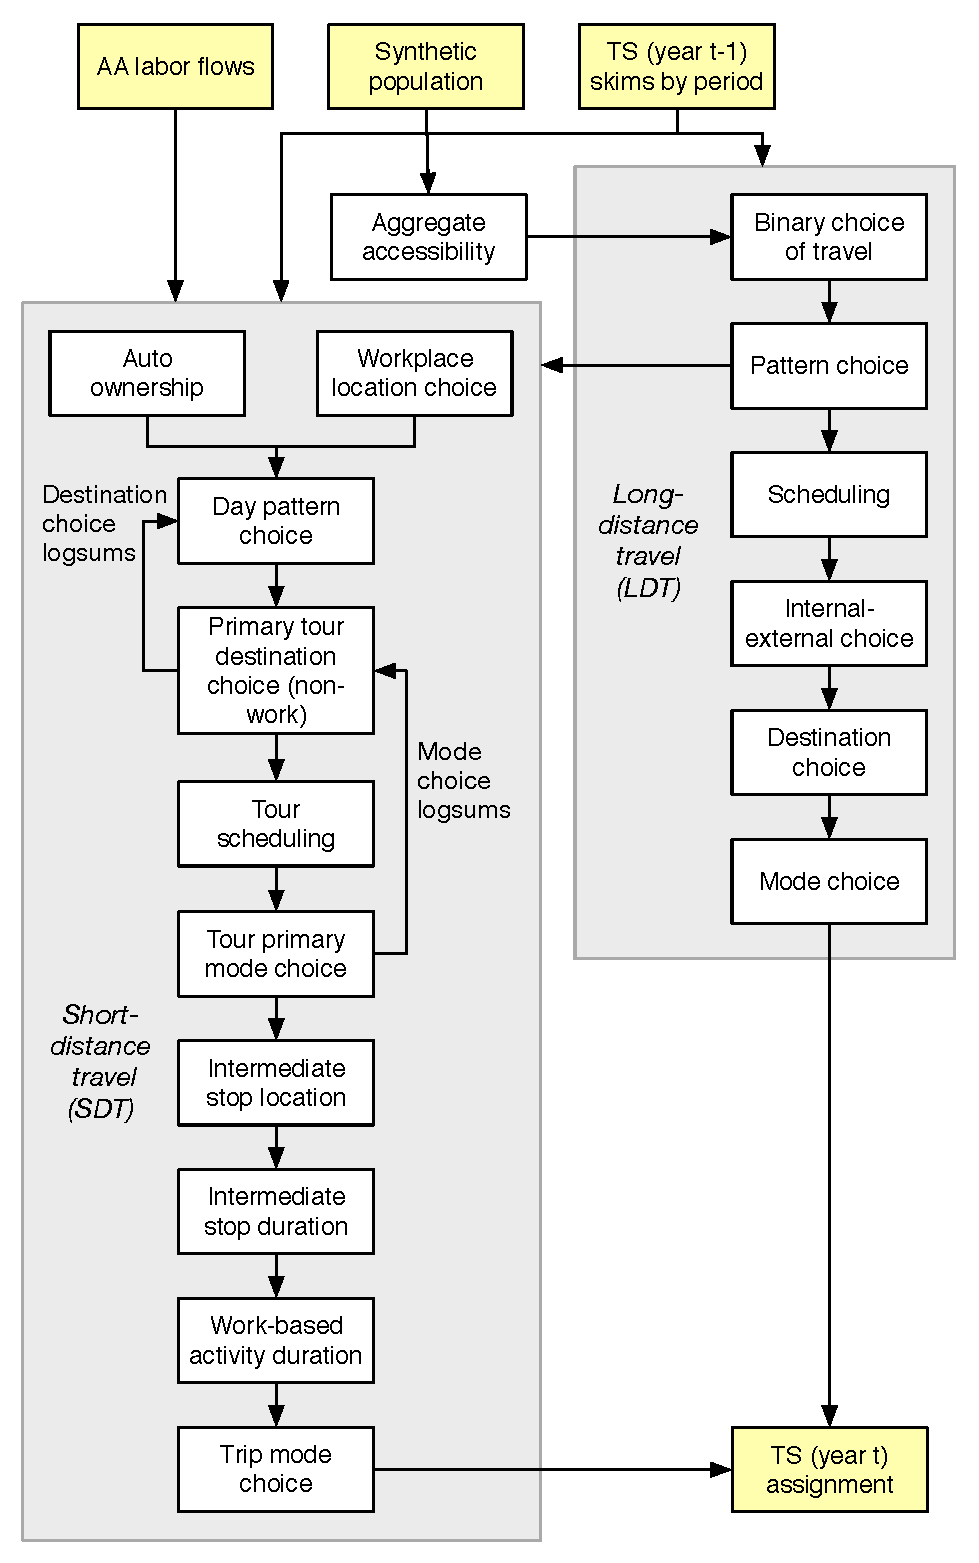
\includegraphics[scale=0.65]{pt/ptmodel}
\caption{Person transport (PT) model flow diagram}\label{fig:ptmodel}
\end{figure}

The SDT model generates mode choice and destination choice logsums as a measure of accessibility for use by the LDT model (and AA module). This allows for a lower probability of long-distance travel if the short-distance destinations are more attractive. In turn, the LDT choice of whether or not to engage in long-distance travel is fed back to the SDT models. Persons who are traveling out-of-town are assumed to not engage in short-distance travel (LDT only) while the remainder are assumed to travel typical short-distance travel patterns (SDT only). 

Short-distance and commute travel (SDT) consist of a series of (mostly) discrete choice models, which represent the trip-making decision as a sequential process, in the following order:  auto ownership, work place location, activity day pattern, primary non-work activity location, work-based activity location, tour schedule, tour mode, intermediate stop location, intermediate stop duration, work-based activity duration and trip mode. 

The behavior of long-distance travel (LDT) is modeled in six steps. First, each eligible traveler is given the choice of whether or not to engage in long-distance travel during a two-week period. For those who travel during the two-week period, the pattern model predicts the type of travel that occurs on the actual simulation day. Third, the tours are scheduled to a time-of-day. Next, each tour is evaluated to determine whether the destination will be internal or external to the model area boundary. Finally, a specific destination and then a mode are chosen.

The resulting trips from both models are assigned together in VISUM to the same networks, although intra-city transit networks are used for SDT trips and inter-city transit networks for LDT trips. PT SDT also outputs prior period mode choice and destination choice logsums based on the prior period's travel costs (skims, 3 year lag) for use in the current year by the PT and the AA module. PT also produces current year synthetic population attributes regarding auto ownership and work alpha zone. 

These PT SDT and LDT components are detailed in the remainder of this section.

\subsection{SDT Aggregate Accessibilities}\label{sec:sdt-aggregate-accessibilities}
Initial aggregate accessibilities are calculated and used by both SDT and LDT components. Tour mode choice logsums and tour destination choice logsums are used as measures of travel accessibility by the LDT and the SDT components of the PT module as well as the AA module. The destination choice logsum represents the overall ability of travelers to access any destination. The logsums are important to PT LDT because they allow the models to capture the effect that people who have access to many destinations within a short distance are less likely to need to make long distance trips. Within SDT, these accessibilities influence the day pattern model, the auto ownership model, the tour destination choice model and the tour scheduling model. They are referred to as aggregate accessibilities because they are a function of the origin and destination zone attributes only. The logsums are calculated in the same fashion as the utilities for the SDT tour mode choice and destination choice model, but excluding all terms that are person-related. The mode choice logsums are however segmented by household market.\footnote{Refer to Sections \ref{sec:sdt-primary-tour-destination} and \ref{sec:sdt-tour-mode-choice} for a detailed description of the PT SDT tour mode choice and destination choice models.}

\subsection{LDT binary choice of travel}
Urban modelers often complain that travel is difficult to predict because it planned on a time scale longer than one day. This is especially true of long-distance travel. To capture this longer-term planning, long-distance tours in LDT are generated over a two-week period, rather than over a single day. The binary choice of travel model, predicts the probability of engaging in each type of long-distance travel during a two-week period. Note that the binary choice of travel model predicts the presence of travel for each purpose (Table \ref{tab:ldt-trip-purposes}) during the time window, not the quantity. The presence could be part of a tour (i.e., departing during the travel window and returning at a later date), it could be a complete tour or it could be multiple tours. Also, an individual can have travel for multiple purposes occur during the two-week window. Given the presence of travel, the LDT tour pattern model will determine what actually happens on the model day. The variables in the linear utility for the binary choice of travel for each purpose include the following:
\begin{itemize}
\item Household attributes (workers, autos, household size, household income, presence of students, single family home)
\item Person attributes (worker occupation, student, sex, age)
\item Accessibility (SDT destination logsums)
\item Constant
\end{itemize}

\subsection{SDT auto ownership model}\label{sec:sdt-auto-ownership}
The PT SDT tour mode choice model requires the number of autos owned by each household. Since the SPG module does not output (not controlled for) auto ownership information in the synthetic population (from SPG2), the PT SDT auto ownership model predicts the total number of vehicles owned by each household. It is a discrete choice multinomial logit model applied to each resident household in the synthetic population. The resulting auto count is output with the household ID for future analysis in addition to other SPG-produced synthetic population attributes. 

In the auto ownership model the household is assigned ownership of zero (base), one, two, or two or more autos. A logit model is used to assign probabilities to the alternative categories for the Monte Carlo process to use in setting this attribute for an individual household. The utility function includes the following variables:
\begin{itemize}
\item Household attributes of composition and wealth (household size, number of employed persons, household income)
\item Accessibility from the home location to the rest of the model area
\item Aggregate destination choice logsum (see Section \ref{sec:sdt-aggregate-accessibilities})
\end{itemize}

The destination choice logsum is calculated as follows, where $p$ denotes an origin zone and $q$ a destination zone:
\begin{equation}\label{eq:7.1}
DCLogsum_p = \sum exp \left[ \alpha \times Dist_{pq} + \beta \times Time_{pq} + log(Emp_q) \right]
\end{equation}
where:
\begin{align*}
DCLogsum_p &= \text{destination choice logsum for home zone $p$ to all destination zones} \\
Dist_{pq} &= \text{distance from zone $p$ to zone $q$} \\
Time_{pq} &= \text{peak period travel time from zone $p$ to zone $q$} \\
Emp_q &= \text{total employment in destination zone $q$} \\
\alpha, \beta &= \text{parameters to be estimated}
\end{align*}

\noindent PT outputs the resulting auto ownership assignment (number of autos) in the household data file, which contains one record per household, as in the synthetic population. 

\subsection{SDT workplace location choice model}\label{sec:sdt-workplace-location-choice}
This model assigns a workplace location for every worker, by sampling from the labor flow probability matrices developed by the AA module. If a work tour is generated for the worker, the work alpha zone chosen through this method will become the primary destination of the work tour and serve as the anchor location for any work-based tours. The workplace location model is applied to each employed person in the synthetic population.

The workplace location (alpha zone) choice for each worker is based on the following factors:
\begin{itemize}
\item Labor dollar flows by occupation between beta zones
\item Quantity of labor produced and consumed in each alpha zone
\item Mode choice logsums, as a measure of travel cost, between alpha zones
\end{itemize}

\noindent The model applies a matrix expansion process to convert labor dollar flows by occupation between beta zones to flows between alpha zones. The formula for this conversion is as follows:
\begin{equation}
F_{a_m} = F_{\beta_{ij}} \times {{QL_m} \over {\sum_{m \in M(i)} QL_m}} \times {QL_n \over {\sum_{n \in N(j)} QL_n}} \times {{exp(\lambda LS_{mn})} \over {\sum_{m \in M(i)} \sum_{n \in N(j)}exp({\lambda LS_{mn}})}}
\end{equation}
where:
\begin{align*}
m &= \text{origin zones in the alpha zone system} \\
n &= \text{destination zones in the alpha zone system} \\
i &= \text{origin zones in the beta zone system} \\
j &= \text{destination zones in the beta zone system} \\
M(i) &= \text{set of all alpha zones contained within a specific beta zone $i$} \\
N(j) &= \text{set of all alpha zones contained within a specific beta zone $j$} \\
F_{mn} &= \text{labor flow from alpha zone $m$ to alpha zone $n$} \\ 
F_{ij} &= \text{labor flow from beta zone $i$ to beta zone $j$} \\
QL_m &= \text{total labor produced at each alpha zone $m$} \\
QL_n &= \text{total labor consumed at each alpha zone $n$} \\
LS_{mn} &= \text{mode choice logsum between alpha zones $m$ and $n$} \\
\lambda &= \text{dispersion parameter} 
\end{align*}

The process applies the above formula to each $ij$ interchange in the activity allocation matrix of labor flows among beta zones, distributing the flow quantity among the corresponding set of $mn$ interchanges. The flow quantities between alpha zones are used to compute flow probabilities for all alpha zone pairs:
\begin{equation}
P_{mn} = F_{a_{mn}} / \sum_{n \in N} F_{a_{mn}}
\end{equation}

The workplace location model uses these probabilities as the likelihood that a worker residing in alpha zone $m$ (a synthetic population attribute) will work in alpha zone $n$. A Monte Carlo process chooses the workplace location based on these flow probabilities.

\subsection{SDT day-pattern model}\label{sec:sdt-day-pattern}
The SDT day pattern models predict the number, purpose and sequence of activities for a given person in the synthetic population generated by SPG2. The following sections discuss the day pattern choice set as well as the various Day Pattern models.

\subsubsection{Day Pattern Choice Set}
As used in PT, a day pattern consists of a sequence of characters, where each character represents an activity. There is one activity per location, implying that a trip is required between each pair of activities in the pattern. The activity purposes handled by the pattern models are described in Table \ref{tab:sdt-tour-def}. The models are segmented by person type, using the five types defined in Table \ref{tab:sdt-person-types}. 

The choice set for each day pattern model consists of the unique day patterns observed for each person type. This choice set was developed from the Ohio Home Interview Survey data. As shown in Table \ref{tab:pt-day-patterns}, approximately one-half of the observed day patterns are observed only once --- see the columns labeled ``Full Day Patterns''. As expected, the most complex day patterns --- those comprising many tours and intermediate stops --- are observed only once or twice. While the models need to be able to reproduce day pattern complexity, including in the choice set a large number of patterns that are chosen only once significantly increases the size of the estimation problem without adding much new information to the models and it is unlikely that the models will be able to uniquely identify each of these patterns. 

\begin{table}
\centering
\caption{Day pattern model choice set size}\label{tab:pt-day-patterns}
\begin{tabular}{lccccccc}
\hline
\multirow{4}{*}{Person type} & \multicolumn{3}{c}{Full day patterns} & & \multicolumn{3}{c}{Generalized day patterns} \\
\cline{2-4}\cline{6-8}
 & & \multicolumn{2}{c}{Unique patterns} & & & \multicolumn{2}{c}{Unique patterns} \\
 & Unique & \multicolumn{2}{c}{observed once} & & Unique & \multicolumn{2}{c}{observed once} \\
\cline{3-4}\cline{7-8}
 & patterns & Frequency & Percent & & patterns & Frequency & Percent \\
\hline
Pre-school & 309 & 168 & 54 & & 177 & 47 & 27 \\
\gray Grade or high school & 426 & 235 & 55 & & 196 & 51 & 26 \\
College & 759 & 525 & 69 & & 383 & 151 & 39 \\
\gray Worker & 2103 & 1,361 & 65 & & 442 & 84 & 19 \\
Non-worker & 942 & 539 & 57 & & 193 & 21 & 11 \\
\hline
\multicolumn{8}{l}{\footnotesize Source: Ohio statewide household interview survey, used in PT estimation. Percentages used in Oregon would be similar.} \\
\end{tabular}
\end{table}

In order to decrease the number of unique day patterns and in particular of those observed only once, day patterns were generalized as follows:
\begin{itemize}
\item If the day pattern consists of one tour, the full specification of the day pattern is retained in the choice set.
\item If the day pattern consists of two tours, the purpose of the intermediate stops is not retained; instead, they are generalized to be of purpose ``Other'' within the pattern choice model; an actual purpose is chosen for each activity in a subsequent model.
\item If the day pattern consists of three or more tours, all intermediate stops are dropped from the pattern specification within the pattern choice model; the actual number of stops is chosen in a subsequent model.
\end{itemize}

These generalizations reduce the choice set as shown in the right half of Table \ref{tab:pt-day-patterns}. In order to retain the ability to predict patterns as complex as those observed in the data, a full day pattern is reconstructed for the cases where the pattern was simplified. Therefore, the activity day pattern models in fact consist of three sets of models:
\begin{itemize}
\item The generalized day pattern models
\item The intermediate stop pattern choice models (assigns number of intermediate stops for 3+ tour patterns)
\item The intermediate stop purpose models (assigns purpose to 2 and 3+ tour patterns)
\end{itemize}

\subsubsection{Generalized day pattern model}
The generalized day pattern models are discrete choice multinomial logit models. Five models were estimated, one for each person type. The estimation file for each model was constructed by including the full choice set as alternatives for each person in the person type set; therefore the number of alternatives for each observation in the estimation size varies with person type and is given by the number of unique patterns (observed in the Ohio statewide data). The base alternative for all the models is the ``Stay-At-Home'' (H) pattern. 

Each of the alternative patterns has an associated identifiable utility consisting of an activity component, a traveler component and a transport component:
\begin{itemize}
\item The activity component includes variables identifying the number and purpose of activities in the pattern, the sequence of activities or tours in the pattern, the number and purpose of tours in the pattern and the number, purpose and presence/absence of intermediate stops in the pattern.
\item The traveler component includes variables that describe the person making the activity day pattern choice, such as age and gender and variables that describe the person's household, such as household size, number of workers, auto ownership, income and presence of young children. Note that worker status and student status are primarily considered via the model segmentation into person types, although they are also used for the person types that allow both conditions (grade/high school students and college students).
\item The transport component includes distance between home and work (for workers) and the destination choice logsum for each tour purpose (the natural log of the denominator of equation \ref{eq:7.4}). The traveler and transport component appear in the models interacted with the activity components.
\end{itemize}

\subsection{SDT stop pattern model}\label{sec:sdt-stop-pattern}
The SDT stop pattern model component assigns the number of intermediate stops to each tour on the generalized day patterns with 3+ tours. It is a discrete choice multinomial logit model, with a choice set that consists of four alternatives:
\begin{itemize}
\item No stops (the base alternative)
\item Outbound stop only
\item Inbound stop only
\item Both one outbound and one inbound stop
\end{itemize} 

\noindent Five models were estimated, one for each tour purpose listed in Table \ref{tab:sdt-tour-def}, with work and work-based purposes combined. The utility of each stop alternative includes travel attribute variables as well as tour and day-pattern composition variables. Since none of the explanatory variables are alternative-specific, they were entered in the utility function with a different coefficient for each alternative; that is, there are no generic coefficients in these models. 

\subsection{SDT intermediate stop purpose model}
The SDT intermediate stop purpose model assigns an activity purpose to the intermediate stops of 2-tour pattern tours and 3+ tour pattern tours. The purpose model component consists of an empirical distribution of activity purposes, derived from home interview survey data. The stop purpose probabilities are based on expanded data. For forecasting, activity purposes are assigned using Monte Carlo simulation. The 2-tour pattern distributions are conditional on the following attributes:
\begin{itemize}
\item Person type
\item Tour purpose
\item Tour number (first or second)
\item Stop position (outbound leg or inbound leg)
\end{itemize}

\noindent The 3+ tour pattern distributions are conditional on the person type, tour purpose, and tour position (first, middle, or last).

\subsection{SDT primary tour destination choice model}\label{sec:sdt-primary-tour-destination}\label{sec:sdt-primary-tour-destination-choice}
This model chooses the location (alpha zone) of the primary destination of a tour, given the known location of the traveler's home. It is a discrete choice multinomial logit model. The choice set for each alternative is the full set of available zonal alternatives, depending on the tour purpose and the type of activities (size term) of the destination TAZ. Destination choice models are very similar to mode choice models in that both are based on the logit discrete choice model. As applied to destination choice models, the logit formulation is:
\begin{equation}\label{eq:7.4}
P_i (k) = {exp(U_{k|i} \over {\sum_{j \in D} exp(U_{j|i})}}
\end{equation}
where:
\begin{align*}
P_i(k) &= \text{probability of selecting destination zone $k$, given origin zone $i$} \\
j \in D &= \text{the unique alternatives (destinations) in the selection set} \\
U_j &= \text{utility of selecting a destination zone, given the origin zone}
\end{align*}

The equation states that given an origin zone $i$, the probability of selecting a destination zone $k$ is a function of the exponential utility of selecting $k$ over the sum of exponential utilities of all attractions zones in the choice set. The larger the utility of travel between origin zone $i$ and destination zone $j$, the greater the probability of travel between the zones.

The utility for a selecting a particular alternative ($U_k$) is a linear function of the attributes that describe the alternative. In a destination choice model, the attributes that describe the selection of a zone include its accessibility, other variables that describe the quality of the choice and variables that describe the quantity of activity in the destination zone:
\begin{equation}\label{eq:7.5}
U_{j|i} = \beta_0 + \beta_1 \times accessibility_{j|i} + \beta_2 \times quality_{j|i} + ln(\beta_3 \times quantity_{j|i})
\end{equation}

Utility functions for destination choice look different from the comparable functions for mode choice models due to the logarithmic term. This term is referred to as the size term. The SDT primary tour destination choice model uses mode choice logsums as a measure of impedance, which has a special interpretation. The destination and mode choice models can be interpreted as sequentially estimated nested models. Mode choice becomes a nested choice under the choice of destination. The coefficient estimated on the mode choice logsum is interpreted as a nesting coefficient. Thus the coefficient must range be between 0 and 1. A value of 1 implies that there is no nesting. A value greater than 1 implies that the nesting order is incorrect.

\subsection{SDT primary tour scheduling model}\label{sec:sdt-primary-tour-scheduling}
This SDT model forecasts simultaneously departure-from-home time and arrival-back-home time for all home-based tours, with a time-of-day resolution of 1 hour. It is a discrete choice multinomial logit model, where the choice set consists of 190 possible schedules:  all possible combinations of 19 departure hours and 19 arrival hours, with the arrival time always greater or equal to the departure time. Early departures or arrivals (before 5:00 AM) are considered a single choice, as are very late departures or arrivals (after 11:00 PM). The base alternative is the most frequent alternative and therefore varies with the tour purpose; it is identified by a zero departure time constant and zero duration constant. The utility function is based on continuous departure time and tour duration shift variables, where departure time is expressed in hours relative to midnight (assigned 0 departure time) and duration is expressed in hours. Three main types of explanatory variables are interacted with the departure time and duration shift variables: 
\begin{itemize}
\item Tour and day pattern variables
\item Traveler attribute variables
\item Travel condition variables
\item Constant term consisting of the sum of a departure time term and a duration term
\end{itemize}

The model is applied to all tours in a day pattern, according to a pre-determined tour priority:  work and school tours are scheduled first, followed by shop tours, then recreational tours and finishing with other tours. Time windows that have been filled with higher priority tours are not available for lower priority tours. Also, if a low priority tour (for example, shop), occurs earlier in the day than a high priority tour (for example, work), then all time windows after the beginning of the work tour are unavailable for the shop tour. When the pattern includes tours of the same priority, they are scheduled sequentially.

\subsection{SDT tour mode choice models}\label{sec:sdt-tour-mode-choice}
The SDT tour mode choice model assigns a primary mode to the entire tour. It uses a generalized definition of mode, which allows a combination of modes for all the trips in the tour. It is a discrete choice nested logit model. The nested structure of the model and its choice set is shown in Figure \ref{fig:sdt-tour-mode-nesting}. A description of the tour mode choice alternatives was given previously in Table \ref{tab:sdt-tour-modes}. The utility associated with any given tour mode choice is a function of the following attributes:
\begin{itemize}
\item Level-of-service components describing the mode for the tour origin and primary destination (e.g., round trip time and cost attributes for origin and primary destination only since intermediate stops not known when this model is applied)
\item Characteristics of the tour (i.e., number of stops)
\item Characteristics of the person choosing the mode
\end{itemize}

%Figure 7.3 Tour Mode Choice Nesting Structure
\begin{figure}
\centering
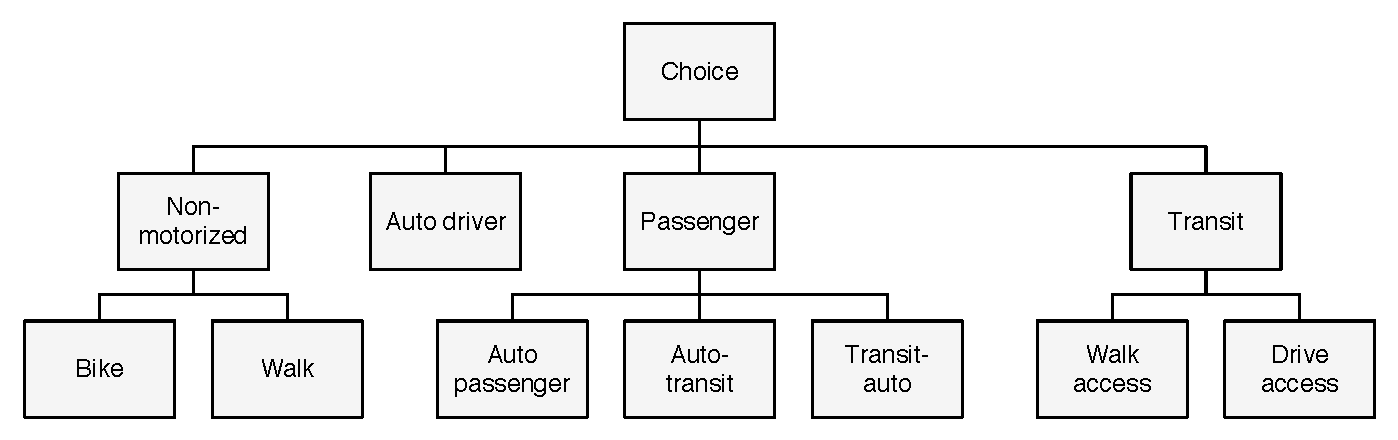
\includegraphics[width=6in]{pt/nesting}
\caption{Tour mode choice nesting structure}\label{fig:sdt-tour-mode-nesting}
\end{figure}

\subsection{Intermediate stop location models}
The PT SDT intermediate stop location model chooses an alpha zone location for each intermediate stop on a tour. It is a discrete choice multinomial logit model, whose utilities are a function of the following attributes:
\begin{itemize}
\item Origin and primary destination of the tour
\item Tour purpose
\item Tour mode
\item Characteristics of each alternative alpha zone location for the stop
\end{itemize}

\noindent The model is structured so that the probability of selecting a TAZ as an intermediate stop destination is inversely related to the out-of-direction travel between the tour origin and its primary destination imposed by its selection. Note this does not preclude intermediate stops to be located farther away from home than the primary destination. The amount of out-of-direction travel is the additional travel time required to reach the intermediate stop using the tour's primary mode; that is, travel time in excess of the time required to travel directly between the tour origin and primary destination. For transit tours, a generalized travel time function is used, to account for out-of-vehicle travel time, as follows:
\begin{equation}
TravelTime_{transit} = InVehicleTime + 1.5 \times FirstWaitTime + 2.5 \times TransferWaitTime + 3.0 \times WalkTime
\end{equation}

Zones that are not reachable by transit (except for the intrazonal alpha zone) are not considered as alternatives for stops on tours whose primary mode is transit.

\subsection{SDT intermediate stop duration models}\label{sec:sdt-intermediate-stop-duration}
The PT SDT intermediate stop duration models predicts the duration of intermediate stops on tours. It is a discrete choice multinomial logit model, where the choice set has a resolution of one hour and includes a total of twelve possible activity durations, ranging from 0-1 hour, 1-2 hours, etc., up to 11 hours or longer. The base alternative is stop duration of one hour or less. The choice set is constrained by the total duration of the tour; that is, alternatives longer than the tour duration are not allowed. The utility function includes daily activity pattern, traveler, and stop attributes. 

\subsection{SDT trip mode choice model}\label{sec:sdt-trip-mode-choice}
The trip mode choice model predicts trip mode, contingent on the previously determined tour mode. The choice set for each trip is determined by the tour mode, as previously shown in Table \ref{tab:sdt-allowable-modes}, and summarized as:
\begin{itemize}
\item If the tour mode is walk, all trips on the tour are walk trips.
\item If the tour mode is bike, all trips on the tour are bike trips.
\item If the tour mode is auto driver, the available trip mode choices are drive-alone, shared ride 2 and shared ride 3+.
\item If the tour mode is auto passenger or the auto passenger leg of a passenger/transit tour, the available trip mode choices are shared ride 2, shared ride 3+ and walk.
\item If the tour mode is walk access transit or the transit leg of a passenger/transit tour, the available trip mode choices are walk to transit and walk. The transit assignment selects the best transit path for this trip.
\item If the tour mode is drive access transit, the first and last trips on the tour are drive to transit trips; other trips are passed to the transit path builder to determine whether the trip mode is walk to transit or walk.
\end{itemize}

Where the trip mode is not uniquely defined by the tour mode nor determined by the transit path builder, the model uses a multinomial discrete choice logit model, with the following attributes:
\begin{itemize}
\item Level of service (in vehicle time, operating cost including parking costs)
\item Household attributes (e.g., household size and income)
\item Alternative specific constants,stratified by tour mode
\end{itemize}

\subsection{SDT work-based activity duration model}
This model forecasts the duration of the three activities that comprise a work based subtour:
\begin{itemize}
\item First at-work activity
\item Primary activity
\item Last at-work activity
\end{itemize} 

\noindent The duration of each individual activity is determined by applying Monte Carlo sampling from a set of empirical distribution functions based on Home Interview data. Two functions describing activity durations were calculated: the proportion of the total tour duration spent at the primary activity and the proportion of the total work activity spent at the first at-work activity. Each of these is described below.

The duration of the primary activity of the work-based subtour is constrained by the total duration of the tour, as follows:
\begin{equation}
PctDuration_{primary} = Duration_{primary} / Duration_{tour}
\label{eq:pt-work-primary-duration}
\end{equation}

\noindent The duration of the first at-work activity duration is constrained by the total duration of the work activity, as follows:
\begin{equation}
PctDuration_{first at-work} = Duration_{first at-work} / Duration_{work}
\label{eq:pt-at-work-duration}
\end{equation}

\noindent PT SDT samples from the frequency tables to obtain the percent duration of the primary and first at-work activities. Given that the duration of the tour is known (exclusive of intermediate stop durations, if present), then the primary and first-at work durations are obtained by solving the equations above and the second at-work duration is obtained as:
\begin{equation}
Duration_{second at-work} = Duration_{tour} - Duration_{primary} - Duration_{first at-work}
\end{equation}

\subsection{LDT tour pattern model}\label{sec:ldt-tour-pattern}
Given the initial LDT long-term choice of travel (LDT rather than SDT, see \S\ref{sec:sdt-aggregate-accessibilities}), LDT next determines if travel occurs on the simulation day and if so what type. The five possible patterns of long distance travel were defined previously in Table \ref{tab:ldt-trip-purposes}. The decision-making agent for household travel is the household and the decision making agent for work-related and other travel purposes is the person.

Because so few travelers take more than one long-distance tour in a single day (one percent in the Ohio long-distance surveys), the tour pattern model does not allow for multiple long-distance tours on the model day. It is not uncommon, however, for travelers to make multiple long-distance tours during the two-week travel window (see \S\ref{sec:sdt-aggregate-accessibilities}), making it more likely that some travel will occur on the model day. Travelers making multiple long-distance tours were included when the tour pattern choice frequencies were developed, such that they implicitly reflect this scenario.

Since the long-distance travel model predicts behavior on a typical weekday, Monday through Thursday, there are no explanatory variables to logically sample among different ``typical weekdays''. Thus, the LDT tour pattern model draws from the observed frequency of each pattern type from along distance travel survey.

\subsection{LDT scheduling model}
LDT tours are scheduled to a time-of-day with a one-hour resolution. Beginning tours are given a departure time, ending tours are given an arrival time and complete tours are given a departure time and duration to fully define their schedule. As with the tour pattern model, the scheduling model draws from observed frequency distributions found in a long distance travel survey.

For complete tours, the schedule is determined using a constants-only logit model, with constants on the departure time and duration. This strategy was applied to smooth the outcomes because observed data was found to have high unexplained variability when viewed in both dimensions.

\subsection{LDT internal-external choice model}\label{sec:ldt-internal-external}
The LDT internal-external choice model is a binary choice model predicting whether a tour will have a destination within the model area or beyond the bounds of the model area. All model coefficients are applied to the utility of leaving the model area. The linear utility function contains the following variables:
\begin{itemize}
\item Household attributes (i.e., income)
\item Person attributes (i.e., occupation, worker binary, age)
\item Complete travel in one day
\item Auto travel time to external station
\item Constant
\end{itemize}

\subsection{LDT destination choice model}
The LDT destination choice models are applied separately for internal versus external destinations. The internal destination choice uses a logit model with utility variables, as specified below:
\begin{itemize}
\item Mode choice logsum
\item Auto travel time (if complete travel in one day)
\item Various size terms (i.e., households, employees, hotel employment, higher education employment, government employment, employment in worker's own industry)
\item Distance flags
\end{itemize}

LDT external destinations cannot be modeled in the same way as internal destination because detailed level-of-service and socioeconomic information are not available outside the model area. Because SWIM2 does not maintain a national network and associated extensive external zone system to associate detailed trip origins and destination, SWIM2 trips are assigned to the selected set of external stations at the edge of the model area (zones numbered in 5000s). Trips are then distributed to the external stations using a simple logit destination choice model with the following utility variables:
\begin{itemize}
\item Highway travel time (as impedance)
\item Traffic volumes at the station (as the size term)
\end{itemize}

\subsection{LDT mode choice model}
The LDT mode choice models include four alternatives in the base year and two optional future year transit options, as shown in Figure \ref{fig:mode-choice-model-nesting-structure}. The base year transit alternatives include walk-to-transit and drive-to-transit alternatives, which cover the existing intercity Greyhound. Amtrak intercity rail service is a separate choice from high-speed rail. The internal model choice model uses a nested logit equation with the following utility variables:
\begin{itemize}
\item Travel/wait time for each trip segment
\item Travel cost as a function of household income
\item Transit nesting coefficients
\item Modal constants
\end{itemize} 

\noindent As with other LDT modules, a simplified mode choice model is applied for trips with destinations outside the model area. In this case, fixed mode splits are applied.

\begin{figure}  % Figure 7.4 Mode Choice Model Nesting Structure
\centering
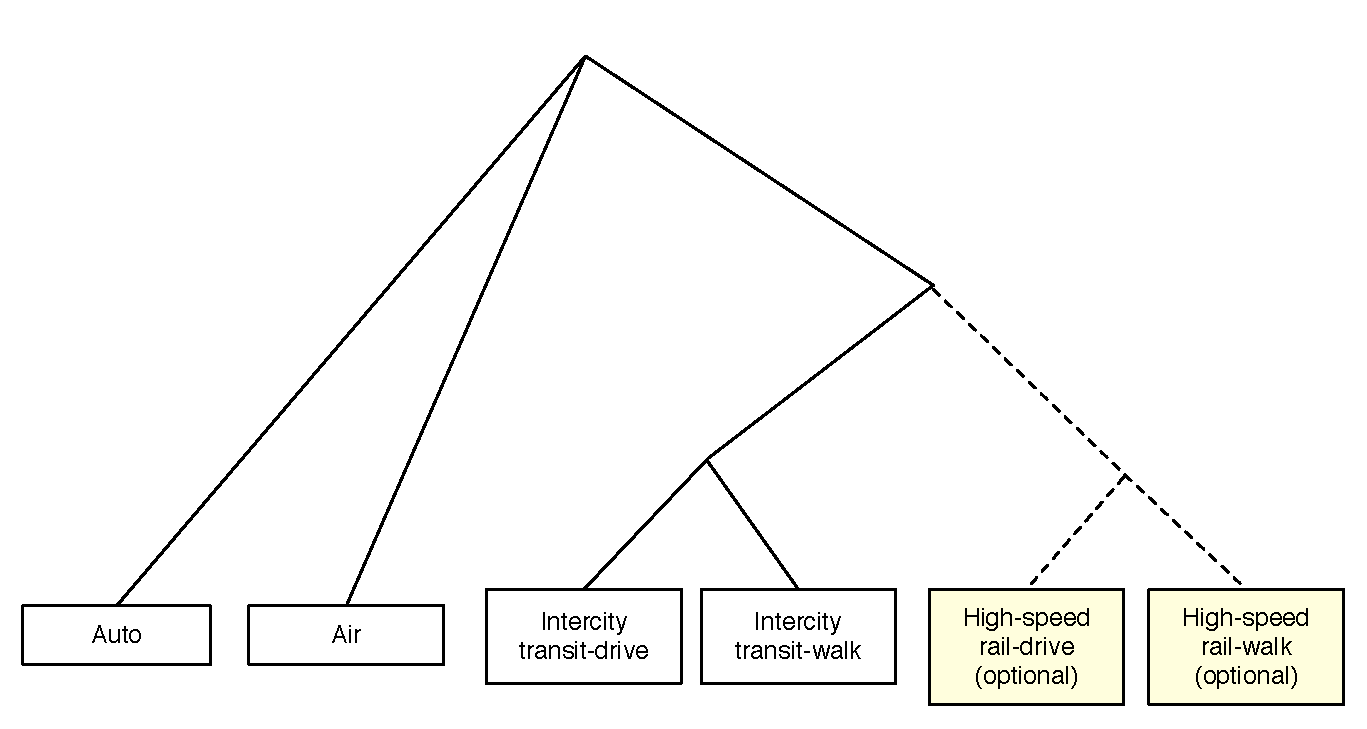
\includegraphics[width=5.5in]{pt/mode-choice-model-nesting-structure}
\caption{LDT mode choice model nesting structure}
\label{fig:mode-choice-model-nesting-structure}
\end{figure}
 
\subsection{Integration}
PT mode choice and destination choice logsums are created at the alpha zone level in compressed zip matrix format. Once PT produces skims at the alpha zone level, it also performs a ``squeeze'' function to produce selected logsum skims at the more disaggregate beta zone level for use in AA. This function will be set to average the component alpha zone values in each beta zone. A weighted average using trip ends will be used once PT is calibrated.

\section{Software implementation}
PT is implemented in the Java programming language, run in a distributed environment across a cluster of computers in order to reduce run times. The model is run in a sequence of steps:
\begin{itemize}
\item Create aggregate mode choice logsums matrices.
\item Create aggregate destination choice logsums matrices.
\item Run auto ownership model for all households.
\item Run workplace location model for all employed persons.
\item Generate a daily pattern of activities for each person by choosing an activity pattern. Each activity implies a nominal location and sequence of activities. Three models are applied to fully specify the day pattern: the generalized pattern model, the stop pattern choice model and the stop purpose model.
\item For each tour in the pattern for each person:
\begin{itemize}
\item Choose the tour schedule: the tour scheduling model for the appropriate tour purpose is applied to select the tour home departure time and the tour duration.
\item Choose a primary destination for the tour: do not choose a destination for work if a location has already been determined in the workplace location model. The tour primary destination choice model for the appropriate tour primary activity is applied to choose a location alpha zone.
\item Choose a primary mode for the tour.
\item Choose a location for each intermediate stop on the tour. The intermediate stop location is a function of the tour primary mode and the location of the tour origin and primary destination.
\item Choose a duration for each intermediate stop on the tour.
\item Choose a trip mode if the tour primary mode is not transit nor the transit leg of a transit-passenger or passenger-transit tour.
\end{itemize}
\item If the tour includes work-based subtours, then for each subtour:
\begin{itemize}
\item Calculate the durations of the three activities that make up the work-based tour, conditional on the duration of the work activity.
\item Calculate the percent of time at the primary destination of the tour
\item Calculate the percent of the at-work portion of the total tour duration that is the first at-work activity.
\item Calculate the duration of the three subtour activities.
\end{itemize}
\end{itemize}

\subsection{PT distributed processing}
Because of the computational requirements of the PT module to micro-simulate a full weekday of activities and travel for several million people within the model area, PT was built to run on a distributed application framework (DAF). The PT-DAF software implementation consists of the following tasks:
\begin{itemize}
\item PTMasterTask
\item MCLogsumCalculatorTask
\item DCLogsumCalculatorTask
\item WorkplaceLocationWorkerTask
\item MicroSimulationWorkerTask
\item LongDistanceTask 
\item Several file writer tasks  
\end{itemize}

\noindent The PTMasterTask, the LongDistanceTask, and the file writer tasks each occupy their own node while the remaining five nodes each have an MC and a DCLogusmCalculator task and multiple MicroSimulationWorkerTasks running on them. 

The PTMasterTask first instructs the MCLogsumCalculatorTasks to calculate a matrix of aggregate mode choice logsums. Although the full mode choice model is applied later, PT pre-calculates an aggregate set of mode choice logsums, which only depend on the activity purpose and market segment. The PTMasterTask sends an activity purpose (Table \ref{tab:sdt-tour-def}) and a market segment (Table \ref{tab:sdt-market-segments}) to each CalculatorTask. The CalculatorTask calculates the logsums for each alpha zone and stores the values in a matrix. The matrices are then passed to the MCWriterTask, which writes the mode choice logsums out to disk in compressed matrix format (Figure \ref{fig:daf-mc-logsums}) for use later by PT (alpha zone) as well as by the AA module (beta zone). 

\begin{figure}
\centering
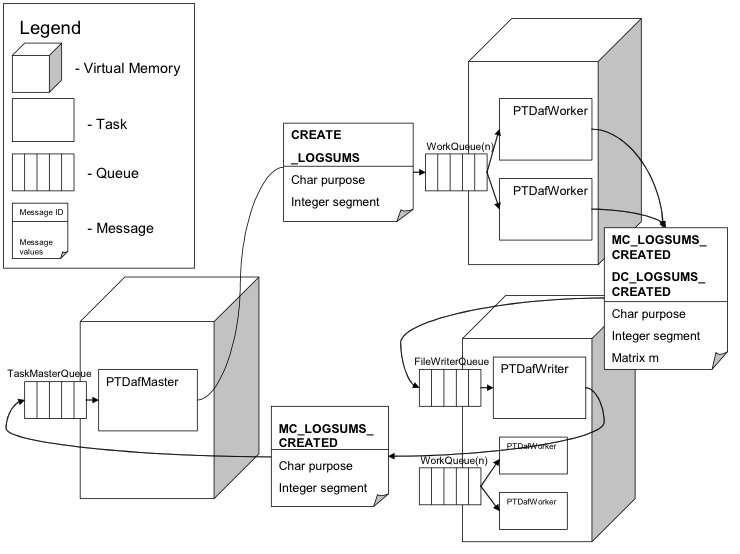
\includegraphics[width=5in]{pt/figure75}
\caption{DAF process to create mode choice logsums}
\label{fig:daf-mc-logsums}
\end{figure}

\begin{figure}
\centering
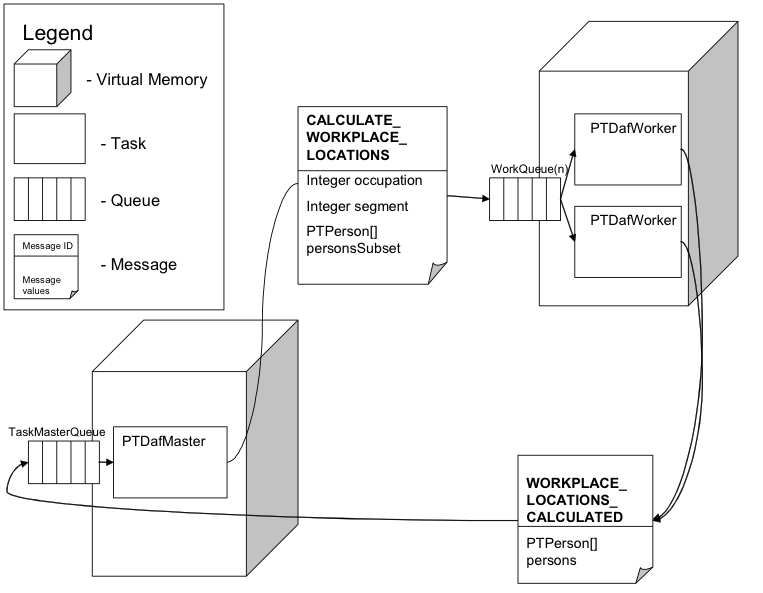
\includegraphics[width=5in]{pt/figure76}
\caption{DAF process to calculate workplace locations}
\label{fig:daf-workplace-location}
\end{figure}

Next the MasterTask assigns each MicroSimulationWorkerTask a set of households to apply the AutoOwnership model to. The full set of households is divided evenly amongst the set of worker tasks. The results are returned to the MasterTask via an array indexed by household ID number. 

Once all the households have been processed, the full array of auto-ownership results is sent back to the Workers so that it can be used in the workplace location model. For this model, the MasterTask assigns each MicroSimulationWorkerTask a set of persons to apply the workplace location model to. The results are sent back to the MasterTask as a mapping between the hhId\_personId (key) and the workplace TAZ (value), as shown in Figure \ref{fig:daf-workplace-location}. In addition, each worker task sends back a summary of its person's employment by occupation by zone to the MasterTask, where it is tabulated and written to disk as Employment.csv. 

After the workplace location model is finished, the destination choice logsums can be calculated. The work is divided up into nine segments so that each DCLogsumCalculatorTask does at least one segment. Before beginning the calculation, each CalculatorTask reads in the latest Employment.csv file and updates their TAZ objects that are used in the size term calculations. The results are sent to the DCWriterTask which creates a table and when the work is completed is written out to disk to be used in future calculations [dclogsums.csv]. 

Once the destination choice logsums are complete, the MasterTask again divides the households evenly amongst the MicroSimulationWorkerTask so the remaining models can be applied. The first set of models in the sequence relate to the long-distance models. Each household decides if the entire household or specific members of the household will make a long distance tour on the model day (long-distance binary choice and long distance pattern choice model). If long-distance tours do occur, Tour objects are formed and sent to the LongDistanceWorkerTask for processing (see LongDistanceWorkerTask description below). The next set of models applied relate to the short-distance travel models. For each household (that does not make a long-distance tour), then for each person (that does not make a long-distance tour), the workers execute the day pattern model, calculating the weekday pattern that determines the person's weekday tours. The workers then loop through each tour and calculate the activity duration, the tour primary destination, tour primary mode choice, intermediate stop destinations, trip mode choice and secondary work-based tour characteristics (duration, destination and mode). 

Once all the members of a household have been processed the worker task sends the Household object (that now contains Person objects that contain Tour objects) to the PTResultsWriterTask where a sequence of files are written to. The outputs written include a Household file [HouseholdData.csv], a Pattern file [WeekdayPattern.csv], a Tour file [WeekdayTour.csv] and most importantly a Trip file [weekdayTrip.csv]. The Trip file is used by VISUM to compile trip matrices by time period for assignment to the network. 

The Long-DistanceWorkerTask applies all of the long-distance models to the tours that were produced by the earlier binary choice models. This includes the scheduling model, the internal/external model, the internal mode and destination choice models, the external mode and destination choice models and the auto details model. Once the tours have been processed, the results are sent to the PTResultsWriterTask which adds the results to LDT specific output files. These include a PersonTour file [ldTours.csv] and a PersonTrips file [ldTrips.csv]. The trips file is used by VISUM in the assignment procedure.

\section{S1 and S2 Module Parameters}\label{sec:pt-s1-s2}
The PT module requires a series of parameters, discussed below by sub-module. Many of the SDT utility function coefficients were originally estimated with the 1995/2000 Ohio Household Survey data, using maximum likelihood methods. In cases, particularly in LDT where the data are unavailable, explanatory variables are insignificant or budget constraints limit analysis, the model components draw from static frequency distributions. LDT estimation was also based on the Ohio Long Distance Travel Survey. These SDT and LDT parameters were adopted in Oregon, adjusting only the utility constants during calibration to Oregon-specific data. In later stages of calibration, mode choice and destination log sums are updated and downstream parameters recalibrated iteratively, until minimal change occurs in this cycle.

Ohio Travel behavior data for the estimation and calibration of the PT SDT models, later transferred to Oregon, were obtained from four home interview surveys and from the 2000 Census. The SWIM2 PT module utility constants were adjusted to match Oregon data:
\begin{itemize}
\item The Ohio Statewide Home Interview Survey, conducted in 2002
\item The OKI Regional Council Home Interview Survey, conducted in 1995
\item The MORPC Home Interview Survey, conducted in 1995
\item The NOACA Home Interview Survey, conducted in 1994
\item 2000 Census Transportation Planning Package
\end{itemize}

\noindent These four surveys comprise a total sample of 26,200 households. The OKI, MORPC and NOACA surveys were re-weighted and re-expanded using Census 2000 data. The surveys were processed to eliminate missing or illogical information, as well as to conform to a unique coding scheme of household, person and trip/activity attributes.

LDT parameter estimation was done for the 2000 Ohio statewide model using the 2002-2003 Ohio Long distance travel survey. These LDT parameters were adopted in Oregon, adjusting only the utility constants during calibration to Oregon-specific data.

\subsection{SDT aggregate accessibilities model estimation}
The aggregate accessibilities used for ``feed-up'' of lower level models to upper level models are mode choice logsums and destination choice logsums. Mode choice logsums are the natural log of the denominator of the mode choice model, which is equivalent to a composite utility of travel across all modes of transportation, weighted by the probability of selection of each mode. Mode choice logsums are created for each household segment and tour purpose and are stored in matrices by origin and destination alpha zone. Destination choice logsums are the natural log of the denominator of the destination choice model, which is equivalent to a composite utility of accessibility across all possible destination zones, weighted by the probability of selection for each TAZ. Since the destination choice model relies on mode choice logsums as the measure of accessibility, the accessibility is based on a consideration of all modes of travel to each zone. Parameters used to produce the PT SDT aggregate accessibilities are the same as those used in the disaggregate SDT tour primary destination choice and tour mode choice components (see Sections \ref{sec:sdt-primary-tour-scheduling} and \ref{sec:sdt-intermediate-stop-location}, respectively). However, since the aggregate accessibilities are pre-computed, certain situational variables, such as number of stops on tour, are not available and are ``turned off'' when computing aggregate accessibilities for upper level components.

\subsection{LDT binary choice of travel model estimation}
The LDT binary choice of travel model predicts if a person will engage in any long distance travel of each purpose during a two-week period. All model coefficients are applied to the utility of traveling. The coefficients were calibrated to match targets for each purpose derived from the Ohio Statewide survey data, but scaled to match total trips from the Oregon element of the 1995 American Travel Survey \citep{bts97}, as shown in Table \ref{tab:ldt-binary-choice-parameters}. The significant descriptive variables are primarily demographic characteristics. Households with more workers and larger households are less likely to travel probably because there are more family ties keeping them home. Households with more autos and higher incomes are more likely to travel due to a higher mobility level and a greater ability to absorb the cost. Certain occupations are more or less likely to travel long-distances, as would be expected. Men are more likely to go on business trips, probably because they tend to have fewer child-care responsibilities. As the short-distance destination choice logsum coefficients indicate, long-distance travel is less necessary if there are more attractive destinations within 50 miles. Finally, individuals who travel with their entire household are less likely to travel on their own. 

\begin{table}[!t]  % 7 8
\centering
\caption{LDT binary choice of travel model parameters}\label{tab:ldt-binary-choice-parameters}
\small
\begin{tabular}{lrrr}
\hline
 & Household & Work-related & Other \\
Variable & coefficients & coefficients & coefficients \\
\hline
Constant & -1.14618 & -6.61398 & -2.06888 \\
\gray Household workers = 1 & -0.3364 &  &  \\
Household workers = 2 & -0.3476 & -0.2928 &  \\
\gray Household workers = 3+ & -1.1494 & -0.3462 &  \\
Household autos = 1 &  &  & 0.419 \\
\gray Household autos = 2 &  &  & 0.606 \\
Household autos = 3+ &  &  & 0.846 \\
\gray Household size = 2 &  &  & -1.149 \\
Household size = 3 & -1.1637 &  & -0.898 \\
\gray Household size = 4+ & -1.4137 &  & -0.809 \\
Household income = \$20-40K & 0.387 &  & 0.289 \\
\gray Household income = \$40-60K & 0.746 &  & 0.417 \\
Household income = \$60K+ & 1.248 & 0.581 & 0.695 \\
\gray Single family dwelling household & 0.254 &  & -0.161 \\
Students = 3+ &  & 0.276 &  \\
\gray Occupation = Agriculture/farming/mining &  &  & -0.636 \\
Occupation = Manufacturing & -0.297 & -0.430 & -0.474 \\
\gray Occupation = Transportation & -0.366 &  & -0.372 \\
Occupation = Wholesale &  & 0.884 &  \\
\gray Occupation = Finance &  & 0.778 &  \\
Occupation = Other services & -0.181 &  & -0.101 \\
\gray Occupation = Professional & -0.3169 &  & -0.1601 \\
College student & -0.242 &  & 0.455 \\
\gray Male &  & 0.806 &  \\
Age &  & 0.100 & 0.051 \\
\gray Age squared &  & -0.001 & -0.001 \\
Short distance destination choice logsum & -0.182 &  & -0.119 \\
\gray Household long distance tour &  & -0.842 & -0.324 \\
\hline
\end{tabular}
\end{table}

\subsection{SDT auto ownership model estimation}
The final estimated SDT auto ownership model discussed in \S\ref{sec:sdt-auto-ownership} is shown in Table \ref{tab:sdt-auto-ownership-parameters}. All variables have significant and logical coefficients. The likelihood of higher auto ownership increases with household size, income, and employed household members. Higher auto ownership decreases with increasing destination choice logsum, meaning that households tend to own fewer cars when they are located near places with high employment. In the destination choice logsum calculation of equation \ref{eq:7.1} the distance coefficient is -0.01835 and the time coefficient is -0.025, parameters $a$ and $b$ in the equation.

\begin{table}   % 7 9
\centering
\caption{SDT auto ownership model parameters}\label{tab:sdt-auto-ownership-parameters}
\small
\begin{tabular}{lrr c rr c rr}
\hline
 & \multicolumn{8}{c}{\textit{Choice alternatives}} \\
 & \multicolumn{2}{c}{One auto} & & \multicolumn{2}{c}{Two autos} &  & \multicolumn{2}{c}{Three+ autos} \\
\cline{2-3}\cline{5-6}\cline{8-9}
Variable & Coefficient & t statistic &  & Coefficient & t statistic &  & Coefficient & t statistic \\
\hline
2 person household & 0.473 & 5.3 &  & 2.845 & 29.8 &  & 2.611 & 23.2 \\
\gray 3+ person household &  &  &  & 2.523 & 44.7 &  & 2.868 & 35.3 \\
Household income = \$20-40K & 1.281 & 15.9 &  & 2.002 & 22.1 &  & 2.225 & 19.2 \\
\gray Household income = \$40-60K & 1.576 & 12.5 &  & 2.995 & 22.7 &  & 3.519 & 23.6 \\
Household income = \$60K+ & 1.658 & 8.1 &  & 3.824 & 18.5 &  & 4.549 & 20.9 \\
\gray 1 household worker & 1.068 & 13.1 &  & 1.226 & 14.0 &  & 1.530 & 15.2 \\
2 household workers & 0.501 & 3.0 &  & 1.723 & 10.3 &  & 2.204 & 12.6 \\
\gray 3+ household workers &  &  &  &  &  &  & 2.731 & 29.8 \\
Destination choice logsum & -0.423 & -6.3 &  & -0.815 & -11.3 &  & -1.280 & -16.8 \\
\gray Constant & 5.811 & 7.1 &  & 7.904 & 9.1 &  & 11.508 & 12.9 \\
\hline
Final likelihood & -21650 &  &  &  &  &  &  &  \\
Rho-squared wrt zero & 0.380 &  &  &  &  &  &  &  \\
Sample size & 25175 &  &  &  &  &  &  &  \\
\hline
\multicolumn{9}{l}{\footnotesize Note:  Estimation using Ohio statewide Home Interview survey. Constants adjusted in Oregon-specific calibration.}
\end{tabular}
\end{table}

\subsection{SDT workplace location choice model estimation}
The only parameter in the SDT workplace location choice model discussed in \S\ref{sec:sdt-workplace-location-choice} is a gravity model dispersion parameter, $\lambda$. It retains the initial value set at 0.54, which was based on a work location choice model that was previously estimated using Oregon household survey data.

\subsection{SDT day-pattern model estimation}\label{sec:pt-day-pattern-estimation}
The estimation results for the five day pattern models discussed in \S\ref{sec:sdt-day-pattern} are summarized in Table \ref{tab:pt-day-pattern-summary}. The detailed listings of variables and parameters estimates are included in Appendix \ref{app:day-pattern-models} (page \pageref{app:day-pattern-models}). 

Among the most powerful explanatory variables across all models are number of tours, presence and/or number of intermediate stops, and number of activities of each purpose. As expected, as the day pattern complexity increases, with complexity measured as either more tours, more activities or more intermediate stops on tours, the less likely the pattern is to be chosen. The models also show that people manage day pattern complexity by trading off number of intermediate stops against number of tours, as shown by the negative coefficients on the product of intermediate stops and tours (see Tables \ref{tab:pt-worker-day-pattern} and \ref{tab:pt-nonworker-person-day-pattern}). % and the negative coefficient on the product of stops on work tours and number of non-work tours (see Table \ref{idunno}).

\begin{table}
\centering
\caption{Day pattern model calibration outcome summary by tour type}
\label{tab:pt-day-pattern-summary}
\begin{tabular}{lrrrl}
\hline
Tour type & Variables & Final likelihood & $\rho^2$ wrt zero & Detailed summary \\
\hline
Pre-school person day pattern & 53 & -11046 & 0.4274 & Table \ref{tab:pt-preschool-person-day-pattern} (page \pageref{tab:pt-preschool-person-day-pattern}) \\
\gray Grade/high school day person pattern & 56 & -27249 & 0.4702 & Table \ref{tab:pt-grade-highschool-person-day-pattern} (page \pageref{tab:pt-grade-highschool-person-day-pattern}) \\
College student day pattern & 90 & 15496 & 0.2780 & Table \ref{tab:pt-college-student-day-pattern} (page \pageref{tab:pt-college-student-day-pattern}) \\
\gray Worker day pattern & 95 & -97414 & 0.3939 & Table \ref{tab:pt-worker-day-pattern} (page \pageref{tab:pt-worker-day-pattern}) \\
Non-worker day pattern & 60 & -97414 & 0.3939 & Table \ref{tab:pt-nonworker-person-day-pattern} (page \pageref{tab:pt-nonworker-person-day-pattern}) \\
\hline
\end{tabular}
\end{table}

The tour sequence variables are also very significant. These variables explain the likelihood of engaging in shop, recreational and other activities before or after work or school, as well as the sequencing of work and school when both activities are part of the day pattern. All models show there is significantly less likelihood of making shop, recreational or other tours before either a school or work tour, with social/recreational tours being less likely to appear before work or school tours than shop tours. 

Both pre-school and grade/high school students are very unlikely to have a day pattern that includes two or more home-based school tours. Grade/high school students are more likely to make a tour that includes both school and work than separate school and work tours. When a work tour is present in their day pattern, it is more likely to appear after the school tour than before. If they self-reported being workers, these students are less likely to choose a pattern that consists of one home-based school tour with no work stops than any other pattern. The likelihood of choosing a day-pattern that includes a work activity is higher for students between 15-17 years old than for younger students. If a school tour has stops, it is most likely to be an inbound stop.

College students are very likely to have a day pattern that is either just a home-based work tour or a home-based school tour without work stops. Patterns that include both school and work tours are also more likely than staying at home, with work after school being the most likely sequence. Patterns with a tour that includes both school and work activities are also more likely than staying at home. And when the day pattern does not include school or work, it is likely to consist of three or more tours, suggesting that the most complex trip-making behavior is left for (or possible on) days that do not include long-duration mandatory activities. Similarly, tours that include both work and school activities are unlikely to have additional stops on it, suggesting limited ability to engage in non-mandatory activities. Outbound stops on work or school tours are very unlikely, while work and school tours with both inbound and outbound stops are more likely than tours with no stops or with only inbound or outbound stops. The same behavior is observed for patterns that include both work and school.

For workers, the most likely pattern consists of a single home-based work tour (no stops) followed by a pattern that includes one work tour (no stops) among other tours. If there are stops on the work tours, inbound stops are more likely than outbound stops. Work-based tours are relatively rare; work-based tours with stops are more likely than work-based tours without stops.

For non-workers the most likely pattern is to stay at home, followed by a single home-based other tour. Their day-pattern is more likely than not to include a recreation tour. When both shop and recreation tours are present in the pattern, the recreation tour is more likely to occur after the shop tour, rather than before. As observed for the other person types, tours with outbound stops are less likely than tours with inbound stops or no stops at all.

The models show multiple, significant and logical effects when the traveler components (age, gender, auto ownership, etc.) are interacted with the activity components:
\begin{itemize}
\item The oldest preschoolers are more likely to engage in out-of-home recreational activities than the youngest children.
\item The likelihood of a school tour increases with preschooler age.
\item Preschoolers are more likely to stay at home if there is a non-working adult in the household or if it is a low income household.
\item Multiple tours or stops on tours are less likely when the household is car-insufficient (owns no cars or owns less cars than adults or workers).
\item Recreational activities (tours or stops) are more likely for persons in high income households.
\item Shopping activities are more likely for persons in high income households.
\item Grade/high school students are less likely to make stops for shop, recreational or other purposes when there is a non-working adult in the household, but more likely to do so when there is only one adult in the household, suggesting sharing of household responsibilities.
\item Grade/high school students are more likely to perform shop tours if they are old enough to drive and there more cars than adults in their household.
\item Female adults are more likely than male adults to engage in shopping activities;
\item When compared against adults 18 to 25 years old, the likelihood of participating in social/recreational activities decreases with age.
\item The youngest adults (18 to 25 years old) are the most likely to stay at home, regardless of whether they are college students, workers or non-workers.
\item Adults with pre-school children at the most likely to stay at home.
\item A worker is less likely to participate in recreational activities if he/she lives in a multiple adult household or if he/she has children.
\item A worker is more likely to have shopping activities if he/she is single and has children.
\end{itemize}

The estimation results for variables that interact accessibility variables with day-pattern composition variables are also significant and logical: 
\begin{itemize}
\item For workers and college students, the likelihood of a multiple tour pattern decreases with increasing home-to-work distance.
\item For college students, the likelihood of making multiple stops on work tours decreases with home to work distance, except when the home is more than 25 miles away from work. Workers are more likely to make stops on their work tours if their home-to-work separation is more than 50 miles. Together, these two results suggest that people tend to decrease stops as their trip length increases, until they reach a distance threshold such that their only way to fulfill their activity needs/desires is by making stops (rather than by performing additional tours).
\item As the destination choice logsum increases (meaning higher accessibility), people are more likely to make more tours and less likely to make stops. They are also less likely to stay at home.
\end{itemize}

\noindent For calibration, the Day-Pattern Model parameters controlling for choice of pattern with respect to specific pattern attributes (i.e., numbers and types of activities on pattern) are considered S2 parameters, the others are S1 parameters.

\subsection{SDT stop pattern and intermediate stop pattern models estimation}
The SDT intermediate stop pattern models include distributions for identification of stop purpose for tours in 2+ tour patterns and a multinomial model for number of intermediate stops for those with 3+ tour patterns by activity type. The trip purpose distributions were derived from Oregon Home Interview Survey data, and are shown in Table \ref{tab:sdt-2t-intermediate-stop-purpose} for 2-stop tour patterns and Table \ref{tab:sdt-3t-intermediate-stop-purpose} for 3+ tour patterns. The stop purpose probabilities are based on expanded data. The distributions are conditional on person type, tour purpose, tour position (3+ tours only), tour number (2 tours only) and tour position (3+ tours only) and stop position (2 tours only). 

The estimation results for the stop choice model, estimated for each tour purpose based upon the Oregon Home Interview Survey, are shown in Table \ref{tab:pt-intermediate-stop-number-models}. It is a discrete choice multinomial logit model with four alternatives, as discussed in \S\ref{sec:sdt-stop-pattern}. Since none of the explanatory variables are alternative-specific, they were entered in the utility function with a different coefficient for each alternative; that is, there are no generic coefficients in these models. A wide range of tour and day-pattern composition variables were tried in all models; only those that resulted in significant coefficients were retained. When a coefficient was made generic across two alternatives, the t-statistic is reported only on one of the alternatives, but the coefficient is reported for both.

\begin{sidewaystable}
\centering
\caption{Two tour intermediate stop purpose model, by market segment}
\label{tab:sdt-2t-intermediate-stop-purpose}
\small
\setlength{\tabcolsep}{3pt}
\begin{tabular}{crrrcrrrcrrrcrrr|rrrcrrrcrrrcrrr}
\hline
 & \multicolumn{15}{c|}{Number of observations} & \multicolumn{15}{c}{Stop purpose probabilities} \\
\cline{2-31}
 & \multicolumn{7}{c}{Tour 1} & & \multicolumn{7}{c|}{Tour 2} & \multicolumn{7}{c}{Tour 1} & & \multicolumn{7}{c}{Tour 2} \\
\cline{2-8}\cline{10-16}\cline{17-23}\cline{25-31}
 Tour & \multicolumn{3}{c}{Outbound} & & \multicolumn{3}{c}{Inbound} & & \multicolumn{3}{c}{Outbound} & & \multicolumn{3}{c|}{Inbound} & \multicolumn{3}{c}{Outbound stops} & & \multicolumn{3}{c}{Inbound stops} & & \multicolumn{3}{c}{Outbound stops} & & \multicolumn{3}{c}{Inbound stops} \\
\cline{2-4}\cline{6-8}\cline{10-12}\cline{14-16}\cline{17-19}\cline{21-23}\cline{25-27}\cline{29-31}
purpose & S & R & O & & S & R & O & & S & R & O & & S & R & O & S & R & O & & S & R & O & & S & R & O & & S & R & O \\
\hline
\multicolumn{31}{l}{\textit{Pre-school persons}} \\ \hline
C & 1 & 5 & 26 & & 9 & 9 & 29 & & 0 & 0 & 2 & & 0 & 0 & 6 & 0.006 & 0.245 & 0.748 & & 0.172 & 0.244 & 0.584 & & 0 & 0 & 1 & & 0 & 0 & 1 \\
\gray S & 9 & 9 & 50 & & 5 & 7 & 26 & & 12 & 15 & 31 & & 3 & 8 & 23 & 0.114 & 0.097 & 0.788 & & 0.107 & 0.161 & 0.732 & & 0.211 & 0.302 & 0.487 & & 0.122 & 0.159 & 0.719 \\
R & & 2 & 15 & & & & 14 & & & 6 & 23 & & & & 22 & & 0.022 & 0.978 & & & 0 & 1 & & & 0.197 & 0.803 & & & 0 & 1 \\
\gray O & & & 27 & & & & 5 & & & & 25 & & & & 5 & & & 1.000 & & & & 1 & & & & 1 & & & & 1 \\
\hline
\multicolumn{31}{l}{\textit{Grade/high school persons}} \\ \hline
W & 0 & 0 & 0 & & 0 & 0 & 0 & & 0 & 1 & 2 & & 1 & 1 & 6 & 0 & 0 & 0 & & 0 & 0 & 0 & & 0 & 0.831 & 0.169 & & 0.046 & 0.073 & 0.881 \\
\gray B & 0 & 0 & 0 & & 0 & 0 & 0 & & 0 & 0 & 0 & & 0 & 0 & 0 & 0 & 0 & 0 & & 0 & 0 & 0 & & 0 & 0 & 0 & & 0 & 0 & 0 \\
C & 7 & 33 & 162 & & 22 & 110 & 209 & & 0 & 3 & 7 & & 4 & 5 & 15 & 0.022 & 0.177 & 0.802 & & 0.051 & 0.334 & 0.615 & & 0 & 0.172 & 0.828 & & 0.084 & 0.247 & 0.669 \\
\gray S & 8 & 7 & 18 & & 3 & 3 & 13 & & 26 & 73 & 87 & & 10 & 33 & 74 & 0.309 & 0.277 & 0.414 & & 0.118 & 0.294 & 0.588 & & 0.115 & 0.371 & 0.515 & & 0.066 & 0.261 & 0.673 \\
R & & 3 & 6 & & & 1 & 12 & & & 47 & 97 & & & 6 & 143 & & 0.144 & 0.856 & & & 0.039 & 0.961 & & & 0.3 & 0.7 & & & 0.051 & 0.949 \\
\gray O & & & 14 & & & & 3 & & & & 57 & & & & 10 & & & 1 & & & & 1 & & & & 1 & & & & 1 \\
\hline
\multicolumn{31}{l}{\textit{College persons}} \\ \hline
W & 5 & 1 & 31 & & 10 & 5 & 42 & & 1 & 3 & 13 & & 5 & 6 & 17 & 0.138 & 0.017 & 0.845 & & 0.11 & 0.174 & 0.715 & & 0.114 & 0.267 & 0.619 & & 0.244 & 0.221 & 0.534 \\
\gray B & 4 & 0 & 4 & & 1 & 2 & 7 & & 0 & 1 & 0 & & 0 & 0 & 2 & 0.334 & 0 & 0.666 & & 0.045 & 0.095 & 0.86 & & 0 & 1 & 1 & & 0 & 0 & 1 \\
C & 0 & 5 & 52 & & 34 & 10 & 69 & & 5 & 2 & 11 & & 9 & 13 & 21 & 0 & 0.049 & 0.951 & & 0.262 & 0.05 & 0.688 & & 0.165 & 0.235 & 0.601 & & 0.226 & 0.225 & 0.549 \\
\gray S & 11 & 5 & 24 & & 3 & 2 & 22 & & 8 & 10 & 35 & & 3 & 16 & 24 & 0.277 & 0.092 & 0.631 & & 0.074 & 0.044 & 0.882 & & 0.128 & 0.178 & 0.694 & & 0.037 & 0.343 & 0.619 \\
R & & & 10 & & & & 9 & & & 17 & 34 & & & 2 & 30 & & 0 & 1 & & & 0 & 1 & & & 0.253 & 0.747 & & & 0.091 & 0.909 \\
\gray O & & & 16 & & & & 3 & & & & 39 & & & & 6 & & & 1 & & & & 1 & & & & 1 & & & & 1 \\
\hline
\multicolumn{31}{l}{\textit{Workers}} \\ \hline
W & 65 & 26 & 589 & & 202 & 91 & 720 & & 26 & 12 & 113 & & 55 & 29 & 136 & 0.074 & 0.038 & 0.888 & & 0.153 & 0.102 & 0.745 & & 0.17 & 0.096 & 0.734 & & 0.235 & 0.115 & 0.65 \\
\gray B & 11 & 0 & 130 & & 46 & 18 & 111 & & 3 & 1 & 7 & & 3 & 3 & 14 & 0.056 & 0.035 & 0.908 & & 0.294 & 0.08 & 0.626 & & 0.157 & 0.019 & 0.824 & & 0.095 & 0.09 & 0.815 \\
S & 51 & 28 & 287 & & 41 & 19 & 149 & & 105 & 102 & 396 & & 32 & 92 & 260 & 0.126 & 0.088 & 0.786 & & 0.167 & 0.097 & 0.736 & & 0.148 & 0.159 & 0.693 & & 0.067 & 0.251 & 0.683 \\
\gray R & & 5 & 42 & & & 4 & 39 & & & 58 & 194 & & & 7 & 191 & & 0.13 & 0.87 & & & 0.1 & 0.9 & & & 0.245 & 0.755 & & & 0.04 & 0.96 \\
O & & & 231 & & & & 60 & & & & 251 & & & & 37 & & & 1 & & & & 1 & & & & 1 & & & & 1 \\
\hline
\multicolumn{31}{l}{\textit{Non-workers}} \\ \hline
\gray S & 111 & 99 & 526 & & 62 & 36 & 266 & & 81 & 56 & 248 & & 26 & 35 & 143 & 0.149 & 0.137 & 0.713 & & 0.16 & 0.128 & 0.712 & & 0.191 & 0.177 & 0.632 & & 0.132 & 0.193 & 0.675 \\
R & & 24 & 94 & & & 4 & 87 & & & 27 & 104 & & & 6 & 120 & & 0.255 & 0.745 & & & 0.042 & 0.958 & & & 0.271 & 0.729 & & & 0.096 & 0.904 \\
\gray O & & & 231 & & & & 51 & & & & 164 & & & & 46 & & & 1 & & & & 1 & & & & 1 & & & & 1 \\
\hline
\multicolumn{31}{l}{\footnotesize Note: Trip purposes are work (W), work-based (B), school (C), shopping (S), recreation (R), and other (O)} \\
\end{tabular}
\end{sidewaystable}


  % Tables 7-15 through 7-19, now combined into single table
\begin{sidewaystable}
\centering
\caption{Three+ tour intermediate stop purpose model, by market segment}
\label{tab:sdt-3t-intermediate-stop-purpose}
\small
\setlength{\tabcolsep}{4pt}
\begin{tabular}{crrrcrrrcrrr|rrrcrrrcrrr}
\hline
 & \multicolumn{11}{c|}{Number of observations} & \multicolumn{11}{c}{Stop purpose probabilities} \\
\cline{2-23}
 & \multicolumn{3}{c}{First tour} & & \multicolumn{3}{c}{Middle tour} & & \multicolumn{3}{c|}{Last tour} & \multicolumn{3}{c}{First tour} & & \multicolumn{3}{c}{Middle tour} & & \multicolumn{3}{c}{Last tour} \\
Tour & \multicolumn{3}{c}{stop purpose} & & \multicolumn{3}{c}{stop purpose} & & \multicolumn{3}{c|}{stop purpose} & \multicolumn{3}{c}{stop purpose} & & \multicolumn{3}{c}{stop purpose} & & \multicolumn{3}{c}{stop purpose} \\
\cline{2-4}\cline{6-8}\cline{10-12}\cline{13-15}\cline{17-19}\cline{21-23}
purpose & ~~S & ~~R & O & & ~~S & ~~R & O & & ~~S & ~~R & O & S & R & O & & S & R & O & & S & R & O \\
\hline
\multicolumn{23}{l}{\textit{Student person types}} \\ \hline
W &  &  &  &  & 1 & 2 & 9 &  & 4 & 6 & 46 &  &  &  &  & 0.3 & 0.085 & 0.615 &  & 0.078 & 0.083 & 0.84 \\
\gray B &  &  &  &  & 0 & 0 & 0 &  & 0 & 0 & 3 &  &  &  &  & 0 & 0 & 0 &  & 0 & 0 & 1 \\
C & 2 & 5 & 12 &  & 9 & 18 & 78 &  & 18 & 14 & 77 & 0.065 & 0.088 & 0.847 &  & 0.065 & 0.12 & 0.815 &  & 0.141 & 0.121 & 0.737 \\
\gray S & 14 & 8 & 86 &  & 19 & 25 & 104 &  & 19 & 16 & 75 & 0.139 & 0.122 & 0.739 &  & 0.063 & 0.167 & 0.77 &  & 0.129 & 0.178 & 0.692 \\
R &  & 2 & 30 &  &  & 10 & 70 &  &  & 11 & 58 &  & 0.029 & 0.971 &  &  & 0.227 & 0.773 &  &  & 0.154 & 0.846 \\
\gray O &  &  & 45 &  &  &  & 55 &  &  &  & 64 &  &  & 1 &  &  &  & 1 &  &  &  & 1 \\
\hline
\multicolumn{23}{l}{\textit{Workers}} \\ \hline
W & 67 & 24 & 328 &  & 44 & 21 & 207 &  & 9 & 5 & 40 & 0.171 & 0.061 & 0.768 &  & 0.132 & 0.057 & 0.81 &  & 0.076 & 0.122 & 0.802 \\
\gray B & 12 & 1 & 42 &  & 2 & 0 & 14 &  & 0 & 0 & 0 & 0.205 & 0.051 & 0.744 &  & 0.058 & 0 & 0.942 &  & 0 & 0 & 0 \\
S & 18 & 19 & 158 &  & 52 & 38 & 283 &  & 35 & 55 & 170 & 0.081 & 0.086 & 0.834 &  & 0.087 & 0.104 & 0.809 &  & 0.181 & 0.178 & 0.641 \\
\gray R &  & 2 & 43 &  &  & 7 & 80 &  &  & 20 & 140 &  & 0.046 & 0.954 &  &  & 0.079 & 0.921 &  &  & 0.079 & 0.921 \\
O &  &  & 121 &  &  &  & 175 &  &  &  & 100 &  &  & 1 &  &  &  & 1 &  &  &  & 1 \\
\hline
\multicolumn{23}{l}{\textit{Non-workers}} \\ \hline
S & 52 & 29 & 257 &  & 57 & 67 & 318 &  & 27 & 33 & 127 & 0.139 & 0.082 & 0.779 &  & 0.113 & 0.172 & 0.715 &  & 0.165 & 0.137 & 0.698 \\
\gray R &  & 5 & 75 &  &  & 5 & 82 &  &  & 10 & 94 &  & 0.062 & 0.938 &  &  & 0.052 & 0.948 &  &  & 0.186 & 0.814 \\
O &  &  & 120 &  &  &  & 156 &  &  &  & 73 &  &  & 1 &  &  &  & 1 &  &  &  & 1 \\
\hline
\multicolumn{23}{l}{\footnotesize Note: Trip purposes are work (W), work-based (B), school (C), shopping (S), recreation (R), and other (O)} \\
\end{tabular}
\end{sidewaystable}


  % Tables 7-20 through 7-22, now combined into single table

% Had to move table definition to after next paragraph to get it to span two
% instead of three pages, but will probably need to re-adjust with all tables

\subsection{SDT primary tour destination choice model estimation}
The estimation results for the SDT tour primary destination choice model discussed in \S\ref{sec:sdt-primary-tour-destination-choice}, including utility expression of equation \ref{eq:7.5}, are shown in Table \ref{tab:pt-primary-destination-choice-models}. All models were estimated using either time and mode choice logsum or distance and mode choice logsums; the latter specification resulted in more logical estimates. The coefficient estimated on the mode choice logsum can be interpreted as a nesting coefficient. Thus the coefficient must range be between zero and one. A value of 1.0 implies that there is no nesting. A value greater than 1.0 implies that the nesting order is incorrect. Logsum coefficients higher than 1.0 in estimation were assigned a value lower than 1.0. The distance variable was stratified by number of tours on the day pattern and by number of stops on tours. The results show that distance decreases with the number of tours, but increases with the number of stops on the tour.

{\setlength{\tabcolsep}{4pt}
\begin{small}
\begin{longtable}{llrrrrrr}
\caption{\normalsize{Intermediate stop number models by tour type}}\vspace{-9pt} \\
\hline 
& & \multicolumn{6}{c}{Choice alternatives}	\\ \cline{3-8}
& & \multicolumn{2}{c}{Outbound} & \multicolumn{2}{c}{Inbound} & \multicolumn{2}{c}{Both} \\
Tour type & Tour stop variable & Coefficient & t statistic & Coefficient & t statistic & Coefficient & t statistic \\ \hline
\endfirsthead
\hline
& & \multicolumn{6}{c}{Choice alternatives}	\\ \cline{3-8}
& & \multicolumn{2}{c}{Outbound} & \multicolumn{2}{c}{Inbound} & \multicolumn{2}{c}{Both} \\
Tour type & Tour stop variable & Coefficient & t statistic & Coefficient & t statistic & Coefficient & t statistic \\ \hline
\endhead
\hline \multicolumn{8}{r}{\emph{Continued on next page}}
\endfoot
\hline
\endlastfoot\label{tab:pt-intermediate-stop-number-models}
Work & Work-based tour dummy & 0.400 & 3.2 &  &  & 0.406 & 2.8 \\
\gray \cellcolor{white} & First work tour in day pattern &  &  & 0.386 & 3.2 & 0.386 &  \\
 & Presence of children$<$5 yrs old & 0.922 & 5.5 &  &  & 0.936 & 4.7 \\
\gray \cellcolor{white} & Presence of children 5-15 yrs old & 0.609 & 4.4 & 0.171 & 1.6 & 0.837 & 5.4 \\
 & Grade/high school person type & -0.342 & -0.9 & -0.342 &  & -1.280 &  \\
\gray \cellcolor{white} & College person type & -0.584 & -2.1 & -0.579 & -2.8 &  &  \\
 & Constant & -2.601 & -19.9 & -1.235 & -12.5 & -2.348 & -18.3 \\ \cline{2-8}
 & Final Likelihood & -2970.931 &  &  &  &  &  \\
 & Rho-Squred wrt Zero & 0.240 &  &  &  &  &  \\
 & Sample Size & 2818 &  &  &  &  &  \\
\hline
School & Four+ tours in day pattern &  &  & -0.481 & -1.6 & -1.076 & -1.4 \\
\gray \cellcolor{white} & First school tour in day pattern & 0.856 & 1.6 &  &  & 1.961 & 1.9 \\
 & Presence of shop tours  &  &  &  &  & -0.820 & -1.8 \\
\gray \cellcolor{white} & Pre-school person type  &  &  & 0.705 & 2.1 & 0.705 &  \\
 & College person type  & 0.890 & 2.9 & 0.728 & 3.6 & 0.788 & 2.2 \\
\gray \cellcolor{white} & Constant & 5.000 & -6.6 & -1.200 & -12.8 & -3.643 & -4.6 \\
\cline{2-8}
 & Final Likelihood & -650.000 &  &  &  &  &  \\
 & Rho-Squred wrt Zero & 0.433 &  &  &  &  &  \\
 & Sample Size & 827 &  &  &  &  &  \\
\hline
Shop & Four or more tours in day pattern & -0.179 & -2.1 & -0.459 & -3.7 & -0.179 &  \\
\gray \cellcolor{white} & Presence of other shop tours & -0.137 & -1.6 &  &  & -0.442 & -3.9 \\
 & Presence of other tours &  &  & 0.251 & 2.2 &  &  \\
\gray \cellcolor{white} & Presence of work or school tours & -0.488 & -4.8 & -0.199 & -1.8 & -0.948 & -7.2 \\
 & Low income household & -0.437 & -2.8 & -0.214 & -1.4 &  &  \\
\gray \cellcolor{white} & Zero car household &  &  &  &  & -1.501 & -1.5 \\
 & Presence of children $<$15 yrs old & 0.408 & 5.0 &  &  & 0.465 & 4.3 \\
\gray \cellcolor{white} & Worker person type & 0.181 & 2.1 &  &  &  &  \\
 & Constant & -1.138 & -4.6 & -1.062 & -10.4 & -1.121 & -8.6 \\
\cline{2-8}
 & Final Likelihood & -4183.000 &  &  &  &  &  \\
 & Rho-Squred wrt Zero & 0.108 &  &  &  &  &  \\
 & Sample Size & 3382 &  &  &  &  &  \\
\hline
Social/ & Four or more tours in day pattern &  &  & -0.513 & -3.0 &  &  \\
\gray \cellcolor{white}recre- & Presence of shop tours & -0.341 & -2.7 &  &  & -0.341 &  \\
ational & Presence of other tours & 0.238 & 1.9 & -0.217 & -1.6 & 0.238 &  \\
\gray \cellcolor{white} & Presence of work or school tours & -0.556 & -3.8 & -0.323 & -2.2 & -0.510 & -2.6 \\
 & Presence of children $<$5 yrs old & 0.458 & 2.5 & 0.358 & 2.1 & 0.365 & 1.6 \\
\gray \cellcolor{white} & Preschool person type & -0.853 & -2.0 &  &  &  &  \\
 & College person type &  &  & 0.735 & 3.2 &  &  \\
\gray \cellcolor{white} & Worker person type &  &  & 0.397 & 2.6 &  &  \\
 & Constant & -1.981 & -11.8 & -1.990 & -13.7 & -3.108 & -14.5 \\
\cline{2-8}
 & Final Likelihood & -2153.000 &  &  &  &  &  \\
 & Rho-Squred wrt Zero & 0.413 &  &  &  &  &  \\
 & Sample Size & 2644 &  &  &  &  &  \\
\hline
Other & Four or more tours in day pattern &  &  &  &  & -0.778 & -3.7 \\
\gray \cellcolor{white} & Presence of shop tours &  &  &  &  & 0.596 & 1.8 \\
 & Presence of other `other' tours &  &  &  &  & 0.759 & 3.1 \\
\gray \cellcolor{white} & Presence of work or school tours & -1.044 & -7.0 & -0.970 & -6.6 & -0.929 & -4.1 \\
 & Presence of children $<$5 yrs old & 0.337 & 3.4 & 0.337 &  &  &  \\
\gray \cellcolor{white} & Presence of children 5-15 yrs old &  &  &  &  & -0.430 & -2.1 \\
 & Grade/high school person type & 0.701 & 2.4 & 0.843 & 3.4 & 0.801 & 1.8 \\
\gray \cellcolor{white} & College person type & 0.475 & 1.8 & 0.424 & 1.7 & 0.992 & 3.0 \\
 & Worker person type & 0.528 & 3.7 & 0.162 & 1.2 & 0.427 & 2.0 \\
\gray \cellcolor{white} & Constant & -2.917 & -30.9 & -1.770 & -31.5 & -3.969 & -15.8 \\
\cline{2-8}
 & Final Likelihood & -3262.000 &  &  &  &  &  \\
 & Rho-Squred wrt Zero & 0.676 &  &  &  &  &  \\
 & Sample Size & 7254 &  &  &  &  &  \\
\end{longtable}
\end{small}
}  % End of tabcolsep override
   % Tables 7-23 through 7-27, now combined
\begin{table}
\centering
\caption{Primary destination choice models by tour type}
\label{tab:pt-primary-destination-choice-models}
\small
\begin{tabular}{l *{8}{r}}
\hline
 & \multicolumn{2}{c}{College education} & & \multicolumn{2}{c}{K12 education} & & \multicolumn{2}{c}{Work-based subtours} \\
\cline{2-3}\cline{5-6}\cline{8-9}
Variable & Coefficient & t statistic & & Coefficient & t statistic & & Coefficient & t statistic \\
\hline
Distance & -0.188 & -12.1 & & -0.698 & -41.0 & & -0.198 & -1.8 \\
\gray ~~~If 2 tours & -0.027 & -2.2 & & -0.004 & -0.4 & & -0.043 & -0.4 \\
~~~If 3+ tours & -0.111 & -5.2 & & -0.068 & -2.8 & & -0.063 & -0.5 \\
\gray ~~~If stops on tour & 0.008 & 0.7 & & 0.038 & 3.6 & & & \\
~~~If preschooler & & & & & & & & \\
\gray Intrazonal indicator & -1.067 & 8.2 & & -0.544 & 31.3 & & -1.014 & 13.7 \\
Mode choice logsum & 0.443 & 4.7 & & 0.453 & 16.7 & & 0.8 (a) & \\
\gray Size terms & & & & & & & & \\
~~~Retail & & & & & & & 1.000 & \\
\gray ~~~Other services & & & & & & & 0.183 & -13.2 \\
~~~Households & & & & & & & 0.208 & -11.7 \\
\gray ~~~Health & & & & & & & 0.059 & -5.8 \\
~~~Transport \& handling & & & & & & & 0.254 & -3.0 \\
\gray ~~~Other employment & & & & & & & 0.005 & -1.9 \\
~~~High ed. employment & 1.000 & & & & & & & \\
\gray ~~~K12 ed. employment & & & & 1.000 & & & & \\
Intrarural indicator & -1.690 & & & -4.270 & & & -5.824 & \\
\hline
Rho-squared wrt zero & 0.130 & & & 0.140 & & & 0.170 & \\
Sample size & 1173 & & & 6808 & & & 2167 & \\
\hline 
\hline
 & \multicolumn{2}{c}{Shop} & & \multicolumn{2}{c}{Social/recreation} & & \multicolumn{2}{c}{Other} \\
\cline{2-3}\cline{5-6}\cline{8-9}
Variable & Coefficient & t statistic & & Coefficient & t statistic & & Coefficient & t statistic \\
\hline
Distance & -0.292 & -48.6 & & -0.197 & -44.7 & & -0.262 & -57.0 \\
\gray ~~~If 2 tours & -0.010 & -2.2 & & -0.036 & -7.0 & & -0.028 & -6.2 \\
~~~If 3+ tours & -0.040 & -6.7 & & -0.049 & -7.9 & & -0.076 & -14.8 \\
\gray ~~~If one stop on tour & 0.059 & 11.3 & & 0.043 & 8.7 & & 0.114 & 23.1 \\
~~~If two stops on tour & 0.115 & 19.1 & & 0.065 & 8.0 & & 0.169 & 20.5 \\
\gray ~~~If preschooler at home & 0.021 & 3.7 & & & & & & \\
Intrazonal indicator & -0.686 & 17.5 & & -0.249 & 24.1 & & -0.628 & 39.8 \\
\gray Mode choice logsum & 0.991 & 20.0 & & 0.76 (a) & & & 0.880 & 20.9 \\
Size terms & & & & & & & & \\
\gray ~~~Retail & 1.000 & & & 1.000 & & & 1.000 & \\
~~~Other services & 0.038 & -30.5 & & 1.755 & 2.7 & & 0.214 & -9.7 \\
\gray ~~~Households & & & & 4.616 & 8.3 & & 1.019 & 0.3 \\
~~~Government & & & & & & & 0.300 & -6.5 \\
\gray ~~~Other employment & & & & & & & & \\
Intrarural indicator & -4.697 & & & -2.515 & & & -3.474 & \\
\hline
Rho-squared wrt zero & 0.130 & & & 0.110 & & & 0.150 & \\
Sample size & 11479 & & & 8582 & & & 15621 & \\
\hline
\multicolumn{7}{l}{\footnotesize (a) Asserted coefficient}
\end{tabular}
\end{table}   % Tables 7-28 and 7-29 combined

\subsection{SDT primary tour scheduling model estimation}\label{sec:sdt-primary-tour-scheduling}
Estimation results for the SDT tour scheduling models discussed in \S\ref{sec:sdt-primary-tour-scheduling} are summarized in Table \ref{tab:sdt-scheduling-models-summary}. The detailed listing of estimated parameters and constants are shown in Appendix \ref{app:sdt-primary-tour-scheduling} (page \pageref{app:sdt-primary-tour-scheduling}), for they cover several pages. A review of those results revealed that the day pattern, traveler attribute and travel condition variables were typically interacted with both departure time shift and duration shift variables; variables were kept if they showed logical estimates for both shift variables and significant estimates for at least one of them.

\begin{table}
\centering
\caption{Summary of tour scheduling models calibration outcomes}
\label{tab:sdt-scheduling-models-summary}
\begin{tabular}{lrrrrl}
\hline
Tour type & Variables & Constants & Final likelihood & $\rho^2$ wrt zero & Detailed results \\
\hline
Work & 73 & 38 & -81685 & 0.2571 & Table \ref{tab:pt-work-tour-scheduling-model} (page \pageref{tab:pt-work-tour-scheduling-model}) \\
\gray School & 66 & 37 & -35633 & 0.3643 & Table \ref{tab:pt-school-tour-scheduling} (page \pageref{tab:pt-school-tour-scheduling}) \\
Shopping & 24 & 38 & -50945 & 0.1743 & Table \ref{tab:pt-shopping-tour-scheduling} (page \pageref{tab:pt-shopping-tour-scheduling}) \\
\gray Social and recreational & 52 & 38 & -36679 & 0.1351 & Table \ref{tab:pt-social-rec-tour-scheduling} (page \pageref{tab:pt-social-rec-tour-scheduling}) \\
\hline
\end{tabular}
\end{table}

The constant terms for all models show the expected result. Increasingly negative departure time or duration constant with decreasing observed departure time or duration frequencies. Among the day-pattern composition variables, those that describe the place of the tour in the pattern sequence relative to the length of the pattern (in tours) are very powerful and have logical signs. The departure time shifts essentially indicate that how early or late, relative to a one-tour pattern, the tour occurs. Note that a non-significant estimate simply means that the tour tends to occur at about the same time as the one-tour pattern. The duration shifts indicates that first tours tend to be the longest tours, followed by second tours, etc. This trend was observed in the data. Note as well that the duration shift variables are negative, indicating that tours in multiple tour patterns are shorter than tours in single tour patterns.

The other day pattern composition variables included in the models are dummy variables to indicate the presence of tours of a given purpose in the pattern and dummy variables to flag the presence of inbound and/or outbound stops in the tour. The models show many significant effects related to these variables, both for tour departure time and for tour duration. For example, the presence of multiple work tours in the day pattern tends to shift work tour departure times early and to shorten the duration of the tour. The presence of tours of any other purpose tends to shift the work tour departure time late and to lengthen the duration of the work tour. Note that this is after controlling for the number of tours in the pattern. The result is logical because it is essentially comparing a work tour coupled with another work tour versus a work tour coupled with a non-work tour; the work tour in the latter case is expected to be longer than the work tour in the former case. The presence of intermediate stops on the tour tends to increase the duration of the tour. However, tours with both inbound and outbound stops are on average shorter than tours with either just one inbound or just one outbound stop (one or the other, depending on purpose), suggesting that when multiple stops occur on a tour they tend to be of short duration.

The models also show multiple significant effects related to the traveler attribute variables. Among these are:
\begin{itemize}
\item Female workers tend to have later work departures and shorter work tours than male workers.
\item The youngest workers (less or equal to 25 years old) tend to have the latest work departures, while the oldest workers (55 years old or older) tend to have the shortest work tours.
\item Workers in the following industries have significantly later departure times for work than workers in all other industries:  arts \& recreation, accommodations \& food, and real estate. Workers in the latter two industries also have the shortest work tours.
\item Persons in worker households tend to make later shop tours than those in no-worker households.
\item Workers and students make longer shop tours than non-workers; women make longer shop tours than men.
\item Workers are more likely to depart late for recreation tours than non-workers or students, but students make the longest recreation tours.
\end{itemize}

The only travel condition variable estimated was tour distance, due to the unavailability of mode choice logsums when the models were estimated. The models show longer tour distance associated with earlier departure times and with longer tours. However, the structure of the models places the scheduling models before the destination choice models for all purposes other than work. Therefore the distance variable can only be used for work tours; for other tour purposes, the distance variable is set to zero. 

\subsection{SDT tour mode choice model estimation}
The SDT tour mode choice model final parameters were asserted rather than estimated in both Ohio and Oregon. An initial set of mode choice model parameters were estimated with the Oregon data. These showed reasonable and significant in-vehicle and out-of-vehicle parameters, but with implied low values of time. Also significant were the number of stops on the tour, showing a direct relationship between the number of stops and the propensity to choose auto driver. To define the final parameters asserted for these models, the in-vehicle time coefficients were set at values consistent with accepted practice, the cost coefficients were set to yield reasonable values of time and other coefficients were adjusted to exhibit similar internal relationships shown by the estimated parameters.

The final parameters are shown in Table \ref{tab:pt-tour-mode-choice-parameters}, and the constants are shown in Table \ref{tab:pt-mode-choice-constants}. All parameter values are given for the mode at the multinomial level. The auto driver mode is the base alternative for each model. Additionally, sets of descriptive statistics are provided, including the implied value of time (cost parameters are in year 2000 cents and time parameters are in minutes) and ratios of in-vehicle time to various out-of-vehicle time parameters. All models have cost parameters stratified by three household income groups.

% Table 7-35 was in two parts, with different number of columns. Thus, I've put
% them into two separate tables rather than trying to cram them into single page
\begin{table}[!t]
\centering
\caption{Tour mode choice model parameters}\label{tab:pt-tour-mode-choice-parameters}
\small
\begin{tabular}{l *{6}{r}}
\hline
Parameter & Work \& college & School & Shop & Recreate & Other & Work-based \\
\hline
In-vehicle time & -0.0250 & -0.0172 & -0.0150 & -0.0150 & -0.0150 & -0.0200 \\
{\vspace{-9pt}} \\
\textit{Cost (cents)} &  &  &  &  &  &  \\
\gray ~~~Low income ($<$\$30k) & -1.0400 & -1.0733 & -0.9360 & -0.9360 & -0.9360 & -1.2480 \\
~~~Med income ($30-$60k) & -0.2600 & -0.2683 & -0.2340 & -0.2340 & -0.2340 & -0.3120 \\
\gray ~~~High income ($>$\$60k) & -0.1300 & -0.1342 & -0.1170 & -0.1170 & -0.1170 & -0.1560 \\
{\vspace{-9pt}} \\
First wait time (2.0) & -0.0500 & -0.0344 & -0.0300 & -0.0300 & -0.0300 & -0.0400 \\
\gray Transfer wait time (2.5) & -0.0625 & -0.0430 & -0.0375 & -0.0375 & -0.0375 & -0.0500 \\
Walk time (2.5) & -0.0625 & -0.0430 & -0.0375 & -0.0375 & -0.0375 & -0.0500 \\
\gray Drive time (2.5) & -0.0625 & -0.0430 & -0.0375 & -0.0375 & -0.0375 & -0.0500 \\
Walk mode time (3.5) & -0.0875 & -0.0602 & -0.0525 & -0.0525 & -0.0525 & -0.0700 \\
\gray Bike mode time (4) & -0.1000 & -0.0688 & -0.0600 & -0.0600 & -0.0600 & -0.0800 \\
{\vspace{-9pt}} \\
\textit{Value of time} &  &  &  &  &  &  \\
~~~Low income ($<$\$30k) & 1.4423 & 0.9615 & 0.9615 & 0.9615 & 0.9615 & 0.9615 \\
\gray ~~~Med income ($30-$60k) & 5.7692 & 3.8462 & 3.8462 & 3.8462 & 3.8462 & 3.8462 \\
~~~High income ($>$\$60k) & 11.5385 & 7.6923 & 7.6923 & 7.6923 & 7.6923 & 7.6923 \\
{\vspace{-9pt}} \\
\textit{Number of stops} &  &  &  &  &  &  \\
\gray ~~~Passenger & -0.6380 & -0.3843 & -0.0867 & -0.1897 & -0.0867 & \\
~~~Walk & -1.6196 & -1.7860 & -1.2873 & -1.2962 & -1.2873 & \\
\gray ~~~Bike & -1.1752 & -1.7846 & -0.7714 & -0.8953 & -0.7714 & \\
~~~Walk-transit & -0.9393 & -0.9790 & -0.2273 & -0.6367 & -0.2273 & \\
\gray ~~~Transit-passenger & -0.1724 & -0.2749 & 0.3845 & -1.5006 & 0.3845 & \\
~~~Passenger-transit & -0.6503 & -0.2749 & 0.1511 & & 0.1511 & \\
\gray ~~~Drive-transit & -2.1832 & & & & & \\
{\vspace{-9pt}} \\
Passenger, hhsize=1 & -0.7148 & & -1.1303 & -1.1917 & -1.1303 & \\
\gray Passenger, hhsize=2 & & 0.8440 & & & & \\
Passenger, hhsize=3 & & 1.4159 & & & & \\
\gray Nesting coefficient & 0.7659 & 0.7659 & 0.7659 & 0.7659 & 0.7659 & 0.7659 \\
\hline
\end{tabular}
\end{table}  % First part (parameters)
\begin{table}[!t]  % Second half of Table 7-35 (has one more column that first half)
\centering
\caption{Tour mode choice model constants}\label{tab:pt-mode-choice-constants}
\small
\begin{tabular}{l *{7}{r}}
\hline
 & \multicolumn{7}{c}{Tour purpose} \\
\cline{2-8}
Variable & Work & School & College & Shop & Recreate & Other & Work subtour \\
\hline
Passenger & 0.0 & 0.0 & 0.0 & 0.0 & 0.0 & 0.0 & -2.51420 \\
~~~Auto$=$0 & 0.0 & 0.0 & 0.0 & 0.0 & 0.0 & 0.0 & 0.0 \\
~~~Auto$<$Workers & -0.80605 & -0.79661 & -0.12926 & -0.65097 & -0.31053 & -1.49818 & 0.0 \\
~~~Auto$\ge$Workers & -2.93411 & -4.70402 & -1.26957 & -1.54200 & -1.26270 & -1.75402 & 0.0 \\
\gray Walk & 0.0 & 0.0 & 0.0 & 0.0 & 0.0 & 0.0 & 2.60870 \\
\gray ~~~Auto$=$00 & 12.06218 & 3.33675 & 8.36162 & 3.42024 & 3.66258 & 3.04538 & 0.0 \\
\gray ~~~Auto$<$Workers & 5.14586 & 3.13756 & 5.61320 & 1.73882 & 2.24566 & 1.36735 & 0.0 \\
\gray ~~~Auto$\ge$Workers & 0.81160 & -1.23361 & 3.15801 & -0.06181 & 1.23595 & 0.19792 & 0.0 \\
Bike & 0.0 & 0.0 & 0.0 & 0.0 & 0.0 & 0.0 & -1.08563 \\
~~~Auto$=$00 & 5.63884 & 1.23757 & 3.12437 & -0.13321 & 0.45245 & 0.23956 & 0.0 \\
~~~Auto$<$Workers & 1.06474 & -0.51173 & 1.69691 & -1.13319 & 0.03291 & -1.69701 & 0.0 \\
~~~Auto$\ge$Workers & -1.86515 & -4.41389 & -0.28726 & -3.29519 & -1.98740 & -3.15621 & 0.0 \\
\gray Walk-Transit & & & & & & & -1.17112 \\
\gray ~~~Auto$=$00 & 10.60363 & 5.16221 & 5.49323 & 2.45280 & 2.60215 & 2.67218 &  \\
\gray ~~~Auto$<$Workers & 2.14506 & 1.12050 & 3.45003 & -0.94705 & -1.57024 & -0.28757 &  \\
\gray ~~~Auto$\ge$Workers & -0.42642 & -4.24694 & 1.00401 & -3.67795 & -2.96557 & -2.86711 &  \\
Transit-Passenger & & & & & & &  \\
~~~Auto$=$00 & 4.34001 & -3.37959 & 0.63602 & -1.87020 & 0.08749 & -0.98882 &  \\
~~~Auto$<$Workers & -0.67127 & -2.15801 & -4.60097 & -3.24972 & -1.50009 & -4.13164 &  \\
~~~Auto$\ge$Workers & -3.50698 & -8.08546 & -1.89834 & -8.62422 & -4.17891 & -4.27614 &  \\
\gray Passenger-Transit & & & & & & &  \\
\gray ~~~Auto$=$00 & 2.01746 & -3.77849 & 1.99748 & -1.49839 & -4.87509 & -1.73966 &  \\
\gray ~~~Auto$<$Workers & -0.72721 & -1.72759 & -5.20397 & -3.88507 & -3.17212 & -3.22580 &  \\
\gray ~~~Auto$\ge$Workers & -3.11437 & -6.27993 & -1.12847 & -14.89020 & -4.39391 & -4.05825 &  \\
Drive-Transit & & & & & & &  \\
~~~Auto$=$00 & -999.00000 & & & & & &  \\
~~~Auto$<$Workers & 1.39641 & & & & & &  \\
~~~Auto$\ge$Workers & -0.04912 & & & & & &  \\
\hline
\end{tabular}
\end{table}   % Second part (constants)

The level of service variables, such as time and cost, represent round trip travel characteristics; that is, they are the sum of the level of service attributes for the outbound and the inbound legs of the tour. Level of service variables are based on the tour origin TAZ and the tour primary destination TAZ; they do not include trips made to intermediate stops on the tour, since the location of these stops is not known when the tour mode choice model is applied.

For calibration, the tour primary mode choice model alternative specific constants are considered S2 parameters, while the others are S1 parameters. 

%Table 7 35 Tour Mode Choice Model Parameters

%TS uses the implied value of time in 2009$ (per [globalTemplate.properties]) as follows:
%userClass.pk.vot = 0.0945 (High Income ($>$\$60K) work purpose)
%userClass.op.vot = 0.0632 (High Income ($>$\$60K) non-work purposes)
 
%Tour Mode Choice Model Parameters (cont)

\subsection{SDT intermediate stop location model estimation}\label{sec:sdt-intermediate-stop-location}
This model was estimated with Oregon data. To construct the estimation file, each alpha zone in the Oregon statewide network was placed into one of 39 districts based on the additional travel time imposed for the alternative zone and the tour origin and primary destination zones, such that an equal number of zones were placed into each district. One alpha zone was then randomly selected within each district, for a total of 39 alternatives plus one chosen alternative. Estimation results for the intermediate stop destination choice models are given in Table \ref{tab:sdt-intermediate-stop-location-estimation}. For calibration, the intermediate stop destination choice model's level-of-service parameters (i.e., out-of-direction time and intrazonal dummies) for all modes are considered S2 parameters, while the others are S1 parameters.

%Table 7 36 SDT Intermediate Stop Location Model Estimation Results
\begin{table}
\centering
\caption{SDT intermediate stop location model estimation results}
\label{tab:sdt-intermediate-stop-location-estimation}
\small
\setlength{\tabcolsep}{4pt}
\begin{tabular}{l *{7}{r}}
{\vspace{-5pt}} \\
\multicolumn{8}{c}{\normalsize{a. Tour purpose on first stop}} \\
\hline
Variable & Work & School & College & Shop & Recreation & Other & Work Based \\
\hline
\multicolumn{8}{l}{\textit{Out of direction time}} \\
~~~Auto & -0.089665 & -0.140456 & -0.093953 & -0.120719 & -0.137263 & -0.175547 & -0.124789 \\
\gray ~~~Walk & -0.040913 & 0.0 & 0.0 & -0.037825 & -0.099832 & -0.492405 & -0.057900 \\
~~~Bike & -0.195644 & -1.029443 & -0.140121 & -1.091560 & 0.099633 & -2.696830 & -0.098721 \\
\gray ~~~Transit & 0.0 & 0.0 & 0.0 & 0.0 & -0.056319 & 0.0 & 0.0 \\
\multicolumn{8}{l}{\textit{Intrazonal indicator origin}} \\
\gray ~~~Auto & 1.065499 & 0.661837 & 0.474727 & 0.896889 & 1.012551 & 1.349375 & 0.918914 \\
~~~Non-motorized & 0.229814 & 1.289337 & 1.499788 & 1.404672 & 0.569464 & -1.065574 & -1.791381 \\
\gray ~~~Transit & 2.364683 & 4.659240 & 2.375588 & 5.000000 & 4.001458 & 3.340845 & 1.947346 \\
\multicolumn{8}{l}{\textit{Intrazonal indicator destination}} \\
~~~Auto & -1.280966 & -0.582351 & -0.804672 & -0.461725 & -0.077896 & 0.032978 & -0.454985 \\
\gray ~~~Non-motorized & 0.253672 & 0.242551 & -1.120175 & 0.367181 & 0.541895 & 0.733409 & -0.411454 \\
~~~Transit & 0.901022 & 1.183129 & 1.499669 & 5.000000 & 2.772157 & 3.401530 & 1.909075 \\
\multicolumn{8}{l}{\textit{Size term}} \\
\gray ~~~Retail LU, all industries & 1.0 & 0.0 & 1.0 & 1.0 & 1.0 & 1.0 & 1.0 \\
~~~Retail LU, retail industry & 0.0 & 1.0 & 1.0 & 0.0 & 0.0 & 0.0 & 0.0 \\
\gray ~~~Retail LU, non-retail industry & 0.0 & 0.484200 & 0.484200 & 0.0 & 0.0 & 0.0 & 0.0 \\
~~~Non Retail & 0.0 & 0.0 & 0.0 & 0.0 & 0.0 & 0.091300 & 0.0 \\
\gray ~~~Grade School & 1.200000 & 0.719400 & 0.719400 & 0.838200 & 0.0 & 0.0 & 1.200000 \\
~~~Households & 0.0 & 0.342100 & 0.342100 & 0.0 & 0.289200 & 0.350700 & 0.0 \\
\hline
{\vspace{-5pt}} \\
\multicolumn{8}{c}{\normalsize{b. Tour purpose for intermediate stop}} \\ \hline
Variable & Work & School & College & Shop & Recreation & Other & Work Based \\
\hline
\multicolumn{8}{l}{\textit{Out of direction time}} \\
~~~Auto & -0.108470 & -0.212940 & -0.119480 & -0.113470 & -0.110090 & -0.145830 & -0.210910 \\
\gray ~~~Walk & -0.040913 & 0.0 & 0.0 & -0.037825 & -0.099832 & -0.492405 & -0.057900 \\
~~~Bike & -0.195644 & -1.029443 & -0.140121 & -1.091560 & 0.099633 & -2.696830 & -0.098721 \\
\gray ~~~Transit & 0.0 & 0.0 & 0.0 & 0.0 & -0.056319 & 0.0 & 0.0 \\
\multicolumn{8}{l}{\textit{Intrazonal indicator origin}} \\
~~~Auto & 0.567788 & 0.012615 & -1.258098 & 0.774427 & 0.205868 & 0.336309 & 0.230082 \\
\gray ~~~Non-motorized & 0.229814 & 1.289337 & 1.499788 & 1.404672 & 0.569464 & -1.065574 & -1.791381 \\
~~~Transit & 2.364683 & 4.659240 & 2.375588 & 5.000000 & 4.001458 & 3.340845 & 1.947346 \\
\multicolumn{8}{l}{\textit{Intrazonal indicator destination}} \\
\gray ~~~Auto & -0.191614 & -0.127197 & 0.123453 & 0.389344 & 1.153131 & 1.092763 & 0.329549 \\
~~~Non-motorized & 0.253672 & 0.242551 & -1.120175 & 0.367181 & 0.541895 & 0.733409 & -0.411454 \\
\gray ~~~Transit & 0.901022 & 1.183129 & 1.499669 & 5.000000 & 2.772157 & 3.401530 & 1.909075 \\
\multicolumn{8}{l}{\textit{Size term}} \\
~~~Retail LU, all industries & 1.0 & 1.0 & 1.0 & 1.0 & 1.0 & 1.0 & 1.0 \\
\gray ~~~Retail LU, retail industry & 0.0 & 1.0 & 1.0 & 0.0 & 0.0 & 0.0 & 0.0 \\
~~~Retail LU, non-retail industry & 0.0 & 0.484200 & 0.484200 & 0.0 & 0.0 & 0.0 & 0.0 \\
\gray ~~~Non Retail & 0.0 & 0.0 & 0.0 & 0.0 & 0.0 & 0.091300 & 0.0 \\
~~~Grade School & 1.200000 & 0.719400 & 0.719400 & 0.838200 & 0.0 & 0.0 & 1.200000 \\
\gray ~~~Households & 0.0 & 0.342100 & 0.342100 & 0.0 & 0.289200 & 0.350700 & 0.0 \\
\hline
\end{tabular}
\end{table}
 
\subsection{SDT intermediate stop duration model estimation}
The estimated model parameters for the SDT intermediate stop duration model discussed in \S\ref{sec:sdt-intermediate-stop-duration} are shown in Table \ref{tab:pt-intermediate-stop-duration-models}. The results show that stop duration increases with deviation distance from the tour anchors; that is, the longer it takes to reach a given stop, the longer the duration of that stop. Stops on shop tours that take place in the morning tend to be longer than stops at any other time of day. Stop duration decreases with increasing number of tours and activities in the daily activity pattern, consistent with the necessary tradeoff of number of activities and activity duration given fixed time budgets. A work tour is highly unlikely to have an intermediate stop longer than six hours, which is also consistent with the notion of fixed time budgets, given the typical long duration of work activities. Note that stops of very long duration (up to 10 hours) may occur for school tours; these are likely to be work activities. The estimation also shows that outbound stops tend to be shorter than inbound stops and that shop stops tend to be shorter than stops for other purposes.

\begin{table}[!t]
\centering
\caption{Intermediate stop duration model parameters}
\label{tab:pt-intermediate-stop-duration-models}
\small
\begin{tabular}{l *7{r}}
\hline
\multirow{2}{*}{Variable} & \multicolumn{7}{c}{Tour Purpose} \\ \cline{2-8}
 & Work & School & College & Shop & Recreation & Other & Work-based \\
\hline
Outbound stop dummy & -0.8000 & -1.2100 & -0.6700 & 0.0900 & -0.0900 & 0.0200 & -1.0300 \\
\gray Tours starts in the morning & -0.6233 &  &  & 0.1520 &  &  & -0.6233 \\
Adult worker dummy &  & 0.3260 & 0.3260 &  &  &  &  \\
{\vspace{-9pt}} \\
\textit{Number of daily tours} \\
\gray ~~~Two &  & -0.2562 & -0.2562 &  & -0.2240 &  &  \\
~~~Three &  &  &  & -0.2124 & -0.4060 &  &  \\
\gray ~~~Three or more &  & -0.4674 & -0.4674 &  &  &  &  \\
~~~Four or more &  &  &  & -0.4403 & -0.7580 &  &  \\
\gray Number of daily stops is 2+ &  &  &  & -0.2975 &  &  &  \\
{\vspace{-9pt}} \\
\textit{Number of daily activities} \\
\gray ~~~Six or seven & -0.1358 &  &  &  &  &  & -0.1358 \\
~~~Six or more &  &  &  &  &  & -0.2231 &  \\
\gray ~~~Eight or more & -0.1640 &  &  &  &  &  &  \\
Presence of shop stops & -0.4323 & -0.5873 & -0.5873 & -0.1710 &  &  & -0.4323 \\
\gray Deviation distance & 0.0086 & 0.0067 & 0.0067 & 0.0069 & 0.0086 & 0.0099 & 0.0086 \\
{\vspace{-9pt}} \\ 
\textit{Constants} \\
\gray ~~~Less than 1 hour & 0.0000 & 0.0000 & 0.0000 & 0.0000 & 0.0000 & 0.0000 & 0.0000 \\
~~~One hour & -0.1818 & -0.4166 & -0.8757 & -1.0337 & -0.4518 & -1.4266 & -0.2276 \\
\gray ~~~Two hours & -0.0734 & -0.4016 & -0.5255 & -1.4073 & -1.2283 & -2.2712 & -0.1220 \\
~~~Three hours & 0.1225 & -1.1849 & -1.3305 & -1.7416 & -1.8994 & -2.6793 & 0.0413 \\
\gray ~~~Four hours & 0.5384 & -1.8436 & -1.7802 & -1.8483 & -2.6073 & -3.1561 & -0.0673 \\
~~~Five hours & 0.2393 & -2.0865 & -3.2447 & -1.4063 & -3.9223 & -5.1640 & -0.3256 \\
\gray ~~~Six hours & 1.1194 & -2.0855 & -1.9475 & -1.6598 & -1.7697 & -8.3657 & -0.6957 \\
~~~Seven hours & 0.7000 & -2.2855 & -2.1475 & -1.8598 & -1.9697 & -8.8657 & -0.8957 \\
\gray ~~~Eight hours & 0.6000 & -2.4855 & -2.3475 & -2.0598 & -2.1697 & -9.3657 & -1.0957 \\
~~~Nine hours & 0.5000 & -2.6855 & -2.5475 & -2.2598 & -2.3697 & -9.8657 & -1.2957 \\
\gray ~~~Ten hours & 0.2000 & -2.8855 & -2.7475 & -2.4598 & -2.5697 & -10.3657 & -1.4957 \\
~~~Eleven hours & 0.1000 & -3.0855 & -2.9475 & -2.6598 & -2.7697 & -10.8657 & -1.6957 \\
\hline
\end{tabular}
\end{table}  % 7 37

For calibration, the alternative-specific constants and the outbound stop indicator (dummy) variable are considered S2 parameters; all others are S1 parameters.
 
\subsection{SDT trip mode choice model estimation}
The estimation of the PT SDT trip mode choice model discussed in \S\ref{sec:sdt-trip-mode-choice} includes the values in Table \ref{tab:sdt-mode-choice-parameters}. The alternative-specific constants in the trip mode choice model are stratified by tour mode. If the tour mode is auto driver, the available trip mode choices are drive-alone, shared-ride 2 and shared-ride 3+. If the tour mode is auto passenger (or the auto passenger leg of a transit/auto passenger tour), the available trip modes are shared-ride 2, shared-ride 3+ and walk. Additionally, there are trip mode choice parameters on travel time, cost (both auto operating and parking) and household size.

For calibration, the trip mode choice model's alternative-specific constants are considered S2 parameters, while the others are S1 parameters. 

\begin{sidewaystable}
\centering
\caption{SDT trip mode choice model parameters}
\label{tab:sdt-mode-choice-parameters}
\small
\begin{tabular}{l *{7}{r}}
\hline
Variable & Work & School & College & Shop & Recreation & Other & Work subtour \\
\hline
In-vehicle time & -0.0137 & -0.0107 & -0.0107 & -0.0134 & -0.0214 & -0.0314 & -0.0182 \\
{\vspace{-9pt}} \\
\multicolumn{8}{l}{\textit{Operating cost if auto driver:}} \\
\gray ~~~Low income ($<$\$30K) & -0.4200 & -0.3700 & -0.3700 & -0.6300 & -0.9500 & -0.6300 & -1.1200 \\
~~~Med income (\$30--60K) & -0.3000 & -0.3700 & -0.3700 & 0.6000 & -0.9500 & 0.6000 & -0.8000 \\
\gray ~~~High income ($>$\$60K) & -0.2100 & -0.3700 & -0.3700 & -0.5800 & -0.9500 & -0.5800 & -0.5600 \\
{\vspace{-9pt}} \\
Operating cost if auto passenger & -0.2300 & -0.6900 & -0.6900 & -0.6000 & -0.9500 & -0.6000 & -0.6111 \\
{\vspace{-9pt}} \\
\multicolumn{8}{l}{\textit{Parking cost if auto driver:}} \\
\gray ~~~Low income ($<$\$30K) & -0.6200 & -0.6600 & -0.6600 & -0.8400 & -0.9500 & -0.8400 & -1.6473 \\
~~~Med income (\$30--60K) & -0.4900 & -0.6600 & -0.6600 & -0.7900 & -0.9500 & -0.7900 & -1.3019 \\
\gray ~~~High income ($>$\$60K) & -0.4900 & -0.6600 & -0.6600 & -0.7900 & -0.9500 & -0.7900 & -1.3019 \\
{\vspace{-9pt}} \\
Shared ride 2, household size 2 & 1.7719 & 1.6602 & 1.6602 & 1.5226 & 1.4822 & 1.5226 & 0.7499 \\
\gray Shared ride 3+, household size 3+ & 2.1331 & 1.9640 & 1.9640 & 1.6402 & 1.4257 & 1.6402 & 0.7499 \\
Shared ride 3+, household size 3+ & 2.1331 & 2.1682 & 2.1682 & 2.8041 & 2.4071 & 2.8041 & 0.2275 \\
\hline
\multicolumn{8}{l}{\textit{Constant if auto driver:}} \\
\gray ~~~Shared ride 2 & -3.5095 & -2.6527 & -2.8170 & -1.9975 & -1.8861 & -1.9552 & -2.6337 \\
~~~Shared ride 3+ & -3.9442 & -3.3369 & -3.3901 & -3.1940 & -2.8310 & -3.1801 & -2.7937 \\
{\vspace{-9pt}} \\
\multicolumn{8}{l}{\textit{Constant if auto passenger:}} \\
\gray ~~~Shared ride 3+ & -0.7093 & 0.1201 & -0.5113 & -0.6926 & -0.4785 & -0.6580 & -0.1991 \\
~~~School bus & 0 & 1.9567 & 0 & 0 & 0 & 0 & 0 \\
\gray ~~~Walk & 1.7979 & 2.1166 & 1.3720 & -0.2075 & 0.7490 & -0.6879 & -1.8716 \\
~~~Transit shared ride 2 & 1.4592 & 4.6664 & -0.3533 & -2.4378 & -4.5688 & -2.0684 & 0 \\
\gray ~~~Transit shared ride 3+ & 0.4644 & 4.8050 & -0.7468 & -5.1960 & -7.1283 & -3.1550 & 0 \\
{\vspace{-9pt}} \\
\multicolumn{8}{l}{\textit{Constant if transit rider:}} \\
~~~Walk & -0.6680 & -2.1328 & -1.8953 & -2.3142 & -1.7179 & -1.3735 & -0.7441 \\
\gray ~~~Transit shared ride 2 & 1.2708 & 1.0859 & 15.5969 & 7.5896 & 2.7324 & -0.8788 & 0 \\
~~~Transit shared ride 3+ & 0.6348 & 2.6636 & 15.0114 & 6.5134 & 2.1380 & -2.8206 & 0 \\
\hline
\end{tabular}
\end{sidewaystable}
  % 7-38
 
\subsection{SDT work-based activity duration model estimation}
The empirical distributions computed for the SDT work-based activity duration model functions described by equations \ref{eq:pt-work-primary-duration} and \ref{eq:pt-at-work-duration} in \S\ref{sec:sdt-trip-mode-choice} are shown below. These functions were obtained from the distribution of activity durations observed in the Oregon Home Interview Survey data. The primary work activity observed frequency distribution (PctDurationprimary) and its observed cumulative distribution functions are shown in Figures \ref{fig:pt-work-based-activity-duration-distributions}(a) and (b), respectively. The corresponding plots for the first at-work activity (PctDurationfirst at-work) are shown in Figures \ref{fig:pt-work-based-activity-duration-distributions}(c) and (d), respectively. 

% Combine Figures 7.7 to 7.10 into single figure
\begin{sidewaysfigure}
\centering
\subfloat[Work-based primary activity]{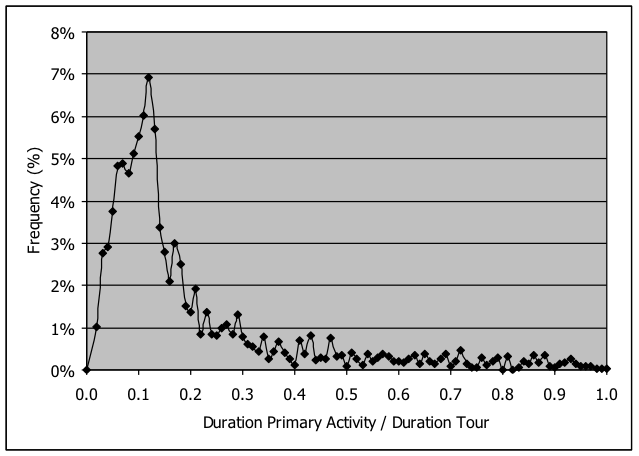
\includegraphics[width = 4in]{pt/excel-figures/figure7-7.png}} 
\subfloat[Cumulative work-based primary activity]{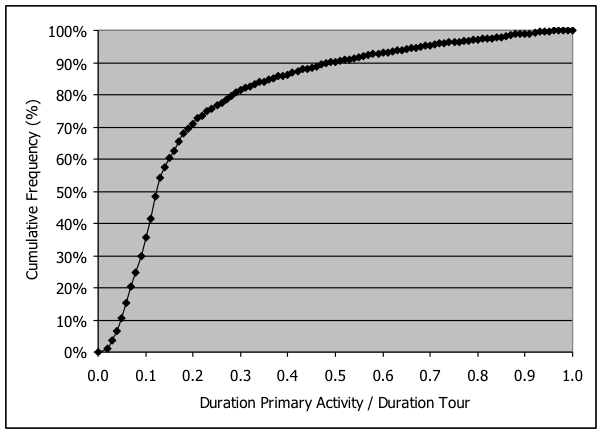
\includegraphics[width = 4in]{pt/excel-figures/figure7-8.png}} \\
\subfloat[First-at-work activity]{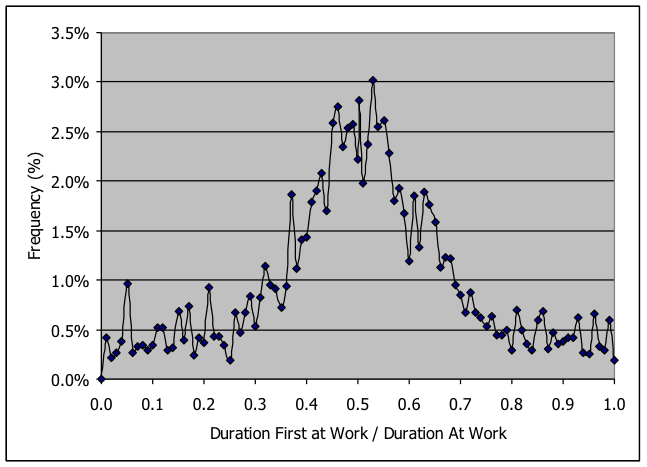
\includegraphics[width = 4in]{pt/excel-figures/figure7-9.png}}
\subfloat[Cumulative first-at-work activity]{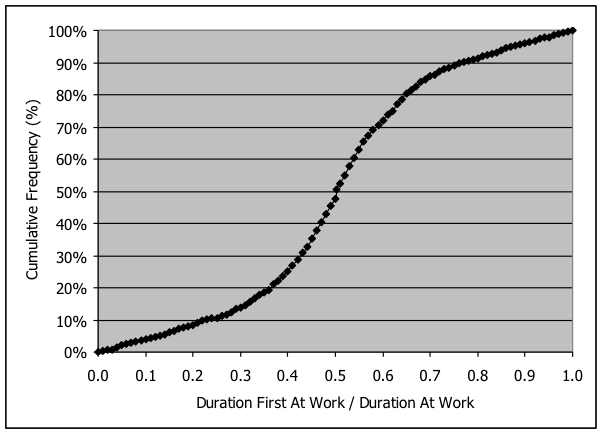
\includegraphics[width = 4in]{pt/excel-figures/figure7-10.png}} 
\caption{Observed frequency distributions for work-based activities}
\label{fig:pt-work-based-activity-duration-distributions}
\end{sidewaysfigure}

\subsection{LDT tour pattern model frequencies}
The LDT tour pattern model discussed in \S\ref{sec:ldt-tour-pattern} predicts the type of long-distance travel that occurs on the simulation day, if any. The model applies a set of factors, by purpose, derived from the Ohio survey data and assumed to be of the same pattern for Oregon. No further calibration is required. 

The Ohio survey-based tour pattern model observed frequency of each pattern type is shown in Table \ref{tab:ldt-tour-frequencies}. Because the model predicts typical weekday (Monday-Thursday) the weekends are excluded and thus work related travel is more likely to occur than household or other travel. Even with Fridays excluded, there are still more travelers departing during the week than returning.

\begin{table}  % 7 39
\centering
\caption{LDT tour pattern choice frequencies}\label{tab:ldt-tour-frequencies}
\begin{tabular}{lccc}
\hline
Pattern type & Household & Work-related & Other \\
\hline
Complete tour & 2.48 & 6.95 & 2.86 \\
\gray Begin tour & 2.37 & 4.72 & 2.11 \\
End tour & 2.03 & 3.36 & 1.71 \\
\gray Away & 7.90 & 11.26 & 5.43 \\
No tour & 85.21 & 73.71 & 87.88 \\
\hline
\multicolumn{3}{l}{\footnotesize Source: Ohio Statewide Model Program, LDT model estimation} \\
\end{tabular}
\end{table}

\subsection{LDT scheduling frequencies}
LDT tours are scheduled to a time-of-day with a one-hour resolution. Beginning tours are given a departure time, ending tours are given an arrival time and complete tours are given a departure time and duration to fully define their schedule. As with the LDT tour pattern model, the scheduling model draws from observed frequency distributions from the Ohio Long Distance Survey data. The Ohio-based departure time distribution for beginning tours and arrival time distribution for ending tours are shown in Figure \ref{fig:ldt-tours-hourly-distribution}. 

\begin{figure}  % 7.11
\centering
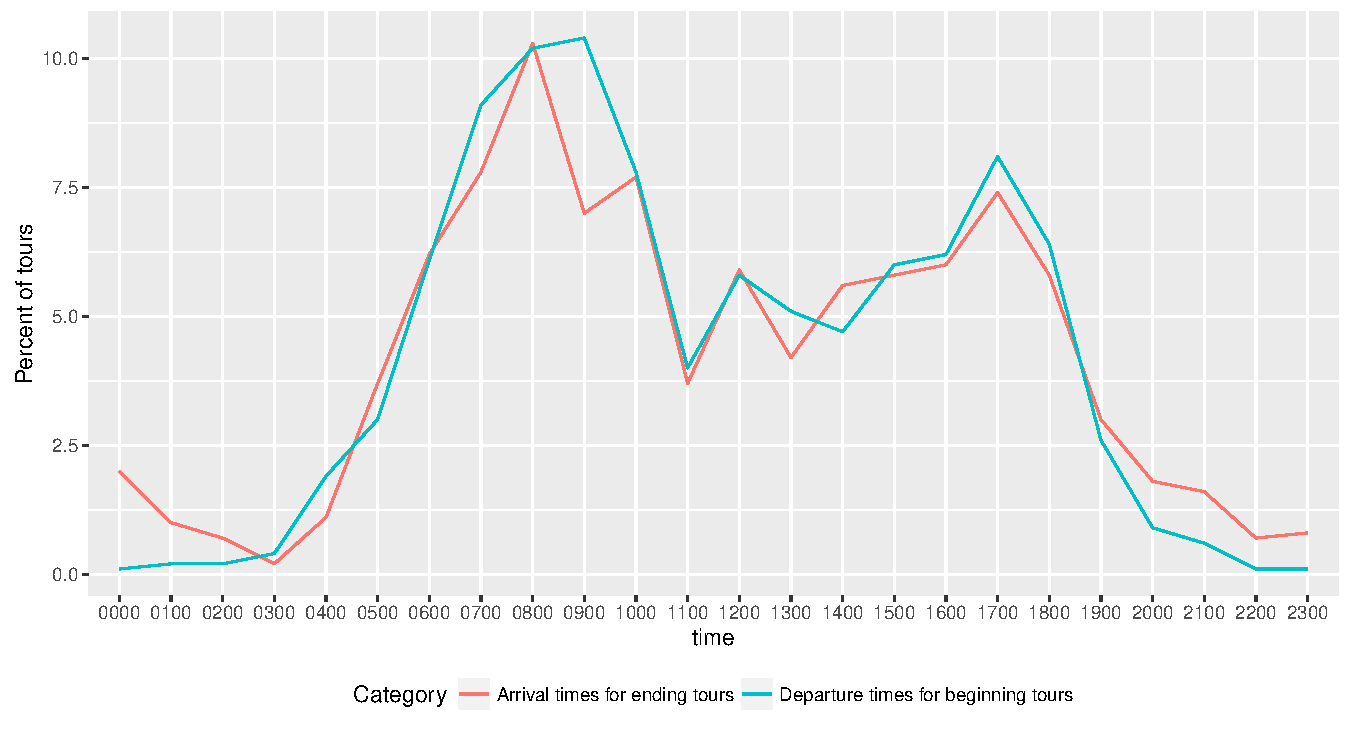
\includegraphics[width=6in, trim=0mm 5mm 0mm 0mm, clip]{pt/tours-hourly-distribution}  % l b r t
\caption{LDT departure times for beginning tours and arrival times for ending tours}
\label{fig:ldt-tours-hourly-distribution}
\end{figure}
 
For complete tours, the schedule is determined using a constants-only logit model, with constants on the departure time and duration. This strategy was applied to smooth the outcomes because the observed data had high unexplained variability when viewed in both dimensions. The choice set is restricted such that trips cannot depart before 5 AM or after 7 PM and all trips must return by 12 AM. The minimum duration is 2 hours and the maximum duration is 17 hours. Some changes were made to the model during calibration to better fit the observed departure time, arrival time and duration distributions. The final model coefficients are shown in Figure \ref{tab:ldt-complete-scheduling-coefficients}. They are estimated such that sequential two-hour periods have the same coefficient, to avoid high variability in the coefficient values. Mornings are popular departure times. The time periods after 3 PM have higher coefficients because the choice set is restricted such that those periods have fewer possible alternatives that can return by 12 AM.

\begin{table}  % 7-40
\centering
\caption{LDT complete tour scheduling model coefficients}\label{tab:ldt-complete-scheduling-coefficients}
\begin{tabular}{lr|lr|lr}
\hline
Variable & Coefficient & Variable & Coefficient & Variable & Coefficient \\
\hline
\multicolumn{2}{l|}{\textit{Duration constant}} & \multicolumn{2}{l|}{\textit{Departure time constant}} & \multicolumn{2}{l}{\textit{Arrival time constant}} \\
2 Hours & 0.959 & 5:00 AM & 0.000 & 9:00 PM & -1.174 \\
\gray 3 Hours & 1.609 & 6:00 AM &  & 10:00 PM & -1.457 \\
4 Hours & 2.544 & 7:00 AM & 1.033 & 11:00 PM & -2.440 \\
\gray 5 Hours & 2.898 & 8:00 AM & 1.944 \\
6 Hours & 3.278 & 9:00 AM & 2.216 &  &  \\
\gray 7 Hours & 3.518 & 10:00 AM & 1.459 \\
8 Hours &  & 11:00 AM & 1.423 &  & \\
\gray 9 Hours & 2.696 & 12:00 PM & \\
10 Hours &  & 1:00 PM & 1.392 &  & \\
\gray 11 Hours & 3.767 & 2:00 PM & \\
12 Hours &  & 3:00 PM & 2.457 &  & \\
\gray 13 Hours & 2.874 & 4:00 PM & \\
14 Hours &  & 5:00 PM & 3.027 &  &  \\
\gray 15 Hours & 2.964 & 6:00 PM & \\
16 Hours &  &  &  &  &  \\
\gray 17 Hours &  & \cellcolor{white} & \cellcolor{white} \\
\hline
\end{tabular}
\end{table}

\subsection{LDT internal-external choice model parameters}
The LDT internal-external choice model discussed in \S\ref{sec:ldt-internal-external} is a binary choice model predicting whether a tour will have a destination within the model area or beyond the bounds of the model area. All model coefficients are applied to the utility of leaving the model area. The models were calibrated to match the in-state versus out-of-state shares found in the Oregon section of the ATS for trips longer than 100 miles. The calibrated values are shown in Table \ref{tab:ldt-internal-external}.

\begin{table}
\centering
\caption{LDT internal-external model estimated coefficients}
\label{tab:ldt-internal-external}
\begin{tabular}{lrrr}
\hline
\multirow{2}{*}{Variable} & Household & Work-related & Other \\
 & coefficients & coefficients & coefficients \\
\hline
Constant & 1.6456 & 2.006 & 0.837 \\
\gray Income $>$\$60K & 0.441 &  &  \\
Occupation $=$ construction &  & -2.892 &  \\
\gray Occupation $=$ finance, insurance, real estate &  & -0.566 &  \\
Occupation $=$ public administration &  & -1.683 &  \\
\gray Occupation $=$ education &  & -1.426 &  \\
Occupation $=$ construction &  & -1.383 &  \\
\gray Person is a worker &  &  & -0.189 \\
Age $<$25 &  &  & -0.319 \\
\gray Age 55+ &  &  & 0.436 \\
Age 65+ &  & -1.155 & 0.436 \\
\gray Complete travel in one day & -2.084 & -2.707 & -1.458 \\
Time to nearest external station & -0.0084 &  & -0.0125 \\
\hline
\end{tabular}
\end{table}


%Table 7 41 LDT Internal-External Model Estimated Coefficients
%Variable       Household
%Coefficients   Work Related
%Coefficients   Other
%Coefficients
%Constant       1.6456  2.006   0.837
%Income <20k                        
%   $20-40k                     
%   $40-60k                     
%   $60k+   0.441           0.462
%Occupation Construction            -2.892      
%   Finance, insurance & real estate            -0.566      
%   Public administration           -1.683      
%   Education           -1.426      
%   Medical         -1.383      
%Person is a Worker                 -0.189
%Age    <25                 -0.319
%   55+                 0.436
%   65+         -1.155  0.436
%Complete Travel in One Day -2.084  -2.707  -1.458
%Time to Nearest External Station   -0.0084     -0.0125

\subsection{LDT destination choice model parameters}
The LDT destination choice models are applied separately for internal versus external destinations. The internal destination choice model parameters calibrated to Ohio trip length data, in the absence of comparable data from Oregon, are shown in Table \ref{tab:ldt-internal-destination-choice-coefficients}. Trips are distributed to external destinations through external stations (zones numbered in the 5000 range) using a simple destination choice model, which uses the highway travel time as the impedance and the traffic volume at the station as the size term. These model coefficients are shown in Table \ref{ldt-ext-dest-coefficients}. 

\begin{table}  % 7-42
\centering
\caption{LDT internal destination choice model estimated coefficients}
\label{tab:ldt-internal-destination-choice-coefficients}
\begin{tabular}{lrrr}
\hline
\multirow{2}{*}{Variable} & Household & Work-related & Other \\
 & coefficients & coefficients & coefficients \\
\hline
Mode choice logsum & 0.936 & 0.612 & 1.000 \\
\gray Time, if complete tour in one day & -0.016 & -0.012 & -0.011 \\
{\vspace{-9pt}} \\
\textit{Size terms} & & & \\
\gray ~~~Total households (a) & 2.793 &  & 1.958 \\
~~~Total employment & 1.000 & 1.000 & 1.000 \\
\gray ~~~Hotel -- if overnight trip (a) & 264.365 & 228.321 & 55.571 \\
~~~Higher education -- if age 18+ and student &  &  & 80.434 \\
\gray ~~~Government employment (a) &  & 7.057 &  \\
~~~Employment in worker's industry (a) &  & 3.671 &  \\
{\vspace{-9pt}} \\
\gray Flag for distance $<$60 miles & -0.167 & 0.286 & -1.514 \\
Flag for distance 60--70 miles & 0.738 & 1.026 & -0.940 \\
\gray Flag for distance 70--150 miles &  &  & -0.349 \\
\hline
\multicolumn{4}{l}{\footnotesize (a) Coefficient for application is exponential of reported coefficient.}
\end{tabular}
\end{table}

\begin{table}  % 7-43
\centering
\caption{LDT external destination choice model estimated coefficients}\label{ldt-ext-dest-coefficients}
\begin{tabular}{lccc}
\hline
\multirow{2}{*}{Variable} & Household & Work-related & Other \\
 & coefficients & coefficients & coefficients \\
\hline
Time & -0.0075 & -0.0075 & -0.0075 \\
\gray Size term (traffic volume) & 1 & 1 & 1 \\
\hline
\end{tabular}
\end{table}

\subsection{LDT mode choice model parameters}
The LDT mode choice model includes six alternatives, as shown in Table \ref{tab:ldt-internal-mode-choice-coefficients}.\footnote{Amtrak occupies the HSR choices in Oregon, a carryover from the Ohio model terminology.} As with destination choice, a simplified mode choice model is applied for trips with destinations outside the model area. In this case, fixed mode splits are applied, as derived from the Oregon segment of the 1995 American Travel Survey (ATS) data. 

\begin{table}  % 7-44
\centering
\caption{LDT internal mode choice model estimated coefficients}
\label{tab:ldt-internal-mode-choice-coefficients}
\begin{tabular}{lrrr}
\hline
 & Household & Work-related & Other \\
Variable & coefficients & coefficients & coefficients \\
\hline
In-vehicle time & -0.005 & -0.010 & -0.005 \\
\gray Walk-access time & -0.010 & -0.020 & -0.010 \\
Drive-access time & -0.010 & -0.020 & -0.010 \\
\gray Wait time -- up to 30 minutes & -0.010 & -0.020 & -0.010 \\
Wait time -- in excess of 30 minutes & -0.003 & -0.005 & -0.003 \\
\gray Cost (cents) -- income \$0-20K & -0.080 & -0.080 & -0.080 \\
Cost (cents) -- income \$20-60K & -0.030 & -0.030 & -0.030 \\
\gray Cost (cents) -- income \$60K+ & -0.012 & -0.012 & -0.012 \\
Transit-high speed rail nest & 0.650 & 0.650 & 0.650 \\
\gray Transit walk-drive nest & 0.500 & 0.500 & 0.500 \\
High speed rail walk-drive nest & 0.500 & 0.500 & 0.500 \\
\hline
\gray Air constant & -3.1870 & -1.0380 & -2.3020 \\
Transit walk access constant & -2.7973 & -2.7973 & -2.7973 \\
\gray Transit drive access constant & -2.7929 & -2.7929 & -2.7929 \\
High speed rail walk access constant & -4.4422 & -4.4422 & -4.4422 \\
\gray High school rail drive access constant & -4.4422 & -4.4422 & -4.4422 \\
\hline
\end{tabular}
\end{table}

\section{Inputs and Outputs}

The PT module inputs and outputs are listed in Tables \ref{tab:pt-generic-inputs} through \ref{tab:ldt-specific-inputs} and \ref{tab:ldt-sdt-outputs}, respectively. PT SDT inputs include the person and household attributes of the synthetic population generated by SPG, labor dollar flows from the AA module, travel attributes from VISUM, all in the current year. PT LDT inputs include external station traffic counts. Additionally, PT SDT and LDT requires some exogenous data including an alpha-to-beta zone mapping file, alpha zone acres and parking costs (daily and hourly), as well as files containing the parameters for each PT model. Currently only the weekday model of PT is used.

The primary PT output is a list of SDT and LDT trip tours for network assignment in VISUM. LDT also prints out an initial output, prior to additional processing into the format used by VISUM for assignment. PT also outputs mode choice and destination choice logsums by alpha zone for its own use and selected beta zone logsums for AA, additional household and person attributes tied to the synthetic population (autos and work location) and an employment summary (based on work location).

% This table is so long and difficult to squeeze to single page that we'll break it into three separate
% tables
\begin{table}  % Table 7-45
\centering
\caption{PT model inputs}\label{tab:pt-generic-inputs}
\begin{tabular}{L{3.2in} L{2.1in} l}
\hline
Data element & File(s) & Source \\
\hline
Lists (with attribute states) of modeled households resident in study area & SynPopH & SPG \\
\gray Lists (with attribute states) of modeled persons resident in study area & SynPopP & SPG \\
Peak and off-peak auto times and distances for interchanges between alpha zones, peak and off-peak walk-to/drive-to transit travel attributes & \*.zmx & VISUM \\
\gray Labor production (home end) and consumption (work end) 2009\$ by occupation in alpha zone & laborDollarProductionSum.csv, laborDollarConsumptionSum.csv & AA \\
Labor selling flows by industry (work trip ends) & selling\_commodity.csv & AA \\
\gray Solved beta zone industry-commodity production and consumption technical coefficients & ZonalMakeUse.csv & AA \\
Alpha zone acres and beta zones in alpha zones & alpha2beta.csv &	Exogenous \\
\gray Unit parking costs (work/nonwork) in alpha zones & alpha2beta.csv: fields ``HourPark'' and ``DayPark'' & Exogenous \\
Size term for LDT destination choice model & ExternalStationVolumes.csv & Exogenous \\
\hline
\end{tabular}
\end{table}

\begin{table}[!t]
\centering
\caption{SDT-specific model inputs}\label{tab:sdt-specific-inputs}
\begin{tabular}{L{2.85in} L{2.45in} l}
\hline
Data element & File(s) & Source \\
\hline
SDT HH survey observed activity patterns & weekdaypatterns.csv, patternAttributes.csv & Exogenous \\
\gray SDT auto ownership model parameters & autoownershipparameters.csv, globalTemplate.properties (latter from distance and time parameters) & Exogenous \\
SDT day pattern model parameters & weekdaypatternparameters.csv, patternparameters.csv & Exogenous \\
\gray SDT intermediate stop purpose model parameters & stoppurpose2tparameters.csv, stoppurpose3ptparameters.csv & Exogenous \\
SDT primary tour scheduling model parameters & TourScheduleParameters.csv & Exogenous \\
\gray Tour mode choice model parameters & tourmodeparameters.csv & Exogenous \\
SDT primary tour destination parameters & tourdestinationparameters.csv & Exogenous \\
\gray SDT intermediate stop model parameters & IntermediateStopChoiceParameters.csv, stopdestinationparameters.csv, firststopdestinationparameters.csv, secondstopdestiatinoparameters.csv & Exogenous \\
SDT trip mode choice model parameters & tripmodeparameters.csv & Exogenous \\
\gray SDT intermediate stop duration model parameters & stopDurationParameters.csv & Exogenous \\
SDT work-based trip duration model parameters & PctWorkBasedDuration.csv & Exogenous \\
\gray SDT cost inputs (walk, bike and drive to transit speeds, auto operating cost, time of first wait segment, non-work parking cost factor) & globalTemplate.properties & Exogenous \\
\hline
\end{tabular}
\end{table}

\begin{table}
\centering
\caption{LDT-specific model inputs}\label{tab:ldt-specific-inputs}
\begin{tabular}{L{2.55in} L{2.8in} l}
\hline
Data element & File(s) & Source \\
\hline
LDT binary choice of travel model parameters & LDTourBinaryChoiceParameters.csv & Exogenous \\
\gray LDT tour pattern model parameters & LDPatternModelFrequencies.csv & Exogenous \\
LDT scheduling model parameters & LDTourScheduleFrequencies.csv, DTourScheduleParameters.csv & Exogenous \\
\gray LDT internal-external choice model parameters & LDInternalExternalParameters.csv, LDExternalDestinationChoiceParameters.csv & Exogenous \\
LDT destination choice model parameters & LDExternalDestinationFrequencies.csv, LDInternalDestinationChoiceParameters.csv & Exogenous \\
\gray LDT mode choice model parameters & LDInternalModeChoiceParameters.csv, LDExternalModeChoiceParameters.csv, LDExternalModeShares.csv & Exogenous \\
LDT other inputs (rental car/taxi/airport parking costs, multi-day trip duration and auto occupancy by purpose) & globalTemplate.properties & Exogenous \\
\hline
\end{tabular}
\end{table}	
  % Table 7 45
\begin{table}  % 7 46
\centering
\caption{SDT and LDT outputs}\label{tab:ldt-sdt-outputs}
\begin{tabular}{L{3.3in} L{1.7in} l}
\hline
Data element & File(s) & Users \\
\hline
Selected mode travel utilities by market segment for interchanges between alpha zones (mode choice logsums) & \#\#mcls.zmx & PT (current year) \\
\gray Selected mode travel utilities by market segment for interchanges between beta zones (mode choice logsums) & \#\#betamcls.zmx & AA \\
Selected destination travel utilities for interchanges between alpha zones (destination choice logsums) & dcLogsums.zmx & PT (current year) \\
\gray Aggregate employment by industry and alpha zone & employment.csv & PT (next year) \\
Additional synthetic population person attributes identified within PT (linked to SynPopP by hhID and personID) & personData.csv & Diagnostics \\
\gray Additional synthetic population household attributes identified within PT (linked to SynPopH by hhID) & householdData.csv & Diagnostics \\
Alpha zone level summary of persons, household, workers & SynPop\_Taz\_Summary.csv & Diagnostics \\
\gray SDT daily pattern details & Patterns\_SDT.csv & Diagnostics \\
SDT person tour and trip details & Trips\_SDTPerson.csv & VISUM \\
\gray LDT person tour details & Tours\_LDT.csv & Diagnostics \\
LDT daily vehicle trips & Trips\_LDTVehicle.csv & Diagnostics \\
\gray LDT daily person trips & Trips\_LDTPerson.csv & VISUM \\
\hline
\end{tabular}
\end{table}
  % Table 7 46

The PT person trip table output used by the VISUM module has the following attributes:
\begin{itemize}
\item Origin alpha zone or external station
\item Destination alpha zone or external station
\item Distance
\item Origin Activity End Time (trip start time)
\item Primary Mode
\item Trip Mode
\end{itemize}

\subsection{Base year time and distance interchange matrices}
PT uses the time and distance interchange matrices (skims) created by VISUM, shown in Table \ref{tab:skims}. During calibration, an exogenous base year set of skims was developed. The base year SWIM2 transit skims were assembled primarily from mid-1990s MPO network data in EMME/2. Peak period skims were created using congested travel times from MPO model runs in the MPO portions of the network and free-flow travel times minus 5 mph in non-MPO areas. Off-peak skims used free-flow speeds. Once the statewide network was built, the skims were generated by EMME/2 using the MPO path-building parameters.
% The base year MPO network data and processing is described further in \ref{37}.

\begin{table}
\centering
\caption{Interchange matrices used by the PT models}\label{tab:skims}
\begin{tabular}{ll}
\hline
\multicolumn{2}{l}{\textit{Separate matrices for the peak and off-peak periods:}} \\
Walk-Transit In-vehicle Time & Drive-Transit In-vehicle Time \\
Walk-Transit First Wait & Drive-Transit First Wait \\
Walk-Transit Total Wait & Drive-Transit Total Wait \\
Walk-Transit Auxiliary Transit (WALK) Time & Drive-Transit Auxiliary Transit (WALK) Time \\
Walk-Transit Number Boardings & Drive-Transit Number Boardings \\
Walk-Transit Fare & Drive-Transit Drive Time \\
\hline
\end{tabular}
\end{table}

Once SWIM2 models are calibrated, the base year skims generated by VISUM replace the original base year inputs synthesized from MPO data. In application, all future year skims are output from VISUM and used in PT in the following (currently three-year) period.

\subsection{Other parameters}
A series of exogenous inputs are provided exogenously in the [globalTemplate.properties] file, under the AO and PT sections. These include the following, including their source data:
\begin{itemize}
\item Auto operating cost (this value is shared by SDT and LDT)
\item SDT speeds, wait time, parking factor: the following speeds and wait times were assumed:
\begin{itemize}
\item Walk speed (mph): 3 mph
\item Bike speed (mph): 12 mph
\item Drive to transit speed (mph): 25 mph
\item Time of first wait segment (minutes): 10 minutes
\item Non-work parking cost factor: 2.5
\end{itemize}
\item LDT-specific travel cost information: in addition to the transit costs associated with network skimming in VISUM, the following long distance travel costs are assumed in LDT. All are expressed in current 2009 dollars.
\begin{itemize}
\item Daily rental car costs: \$71.60/day
\item Taxi rate: \$2.15/minute
\item Daily airport parking costs: \$16.37/day
\end{itemize}
\item LDT average duration of a multi-day trip by purpose: 2.4, 4.6, and 2.6 hours for household, work-related, and other purpose, respectively.
\item LDT average auto occupancy by purpose, based upon the Ohio Long Distance Survey: 2.81, 1.22, and 1.91 hours for household, work-related, and other purpose, respectively.
\end{itemize}

\section{Calibration Targets}
During initial calibration, the PT module was formally compared to 14 sets of observed targets, to include household travel surveys, listed in Table \ref{tab:pt-calibration-targets}. Supplemental calibration targets are also listed. Transit boarding data from the major transit agencies in the state (typically annual or monthly boardings system-wide and/or by route) were compared with daily transit trips output by PT and VISUM. Census Journey to Work data commute trips (at a sub-county geographic scale) were used by PT (and AA) to calibrate the PT generated work trips (and AA labor flows).

\begin{sidewaystable}  % 7 47
\centering
\caption{PT calibration targets}\label{tab:pt-calibration-targets}
\begin{tabular}{lll}
\hline
Model & Source & SWIM2 targets \\
\hline
SDT & 1994/96 Oregon Travel & Average tours by purpose and MPO per household day \\
    & Behavior Surveys & Frequency of patterns by number of tours per pattern and MPO \\
    & & Average number of trips per household by MPO \\
    & & Frequency of tour departure time and duration and hour by MPO \\
    & & Average highway distance by tour purpose and MPO \\
\hline
SDT & 1990 and 2000 Census Journey & Commute trip data \\
    & to Work data \\
\hline
SDT & Local transit boarding data$^a$ & 1990 monthly passenger boardings \\
    & & July 1987--December 1999 (--August 1998 by route) monthly passengers \\
    & & 1987-96 average weekday boardings by route \\
    & & 1991-99 monthly ridership totals \\
    & & 1993 service performance and ridership by route \\
\hline
LDT & 1995 American Travel Survey & Number of trips $>$100 miles made by Oregon residents \\
    & Oregon element & Share of long-distance trips remaining within Oregon \\
    & & Share of auto versus non-auto long-distance trips \\
\hline
\multicolumn{3}{l}{\footnotesize a. Data provided by Tri-Met, Lane TD, Salem-Kaiser Transit, and Rogue Valley Transit.}
\end{tabular}
\end{sidewaystable}

\subsection{Initial calibration}
The PT module was updated in fall 2006 to add the LDT component and update various SDT components enhanced in Ohio application. After code changes were made, both the SDT and LDT components completed S2 calibration, in isolation of other modules. 

\subsection{SDT calibration}
The initial calibration of the SDT component of PT was based on a five percent population sample model estimates. The results were factored by the sampling rate so they are representative of the entire population. Once the model was well-calibrated, a 100 percent population run was completed and the results were compared to the target data.

\subsubsection{Day-pattern choice model}
The PT day-pattern choice model was calibrated to match the targets shown below. The PT parameters control for the choice of pattern with respect to specific pattern attributes (i.e., numbers and types of activities on pattern) for each person type. 
The calibration results for the distribution of patterns by the number of tours in the pattern, for all of Oregon plus Clark County in Washington and MPO regions, are shown in Table \ref{tab:patterns-by-number-of-tours}. The model matches the targets in terms of total patterns produced, statewide and by MPO region. It tends to over-predict the longest patterns, which are also the least frequent ones.

\begin{small}
\begin{longtable}{lcrrrrrr}
\caption{\normalsize{Patterns by number of tours per pattern}}\vspace{-9pt} \\ 
\hline
 & Number & \multicolumn{2}{c}{Target} & \multicolumn{2}{c}{Estimate} & \multicolumn{2}{c}{Error} \\
\cline{3-4}\cline{5-6}\cline{7-8}
Area & of tours & Frequency & Percent & Frequency & Percent & Frequency & Percent \\
\hline
\endfirsthead
\hline
 & Number & \multicolumn{2}{c}{Target} & \multicolumn{2}{c}{Estimate} & \multicolumn{2}{c}{Error} \\
\cline{3-4}\cline{5-6}\cline{7-8}
Area & of tours & Frequency & Percent & Frequency & Percent & Frequency & Percent \\
\hline
\endhead
\hline \multicolumn{8}{r}{\emph{Continued on next page}}
\endfoot
\hline
\endlastfoot\label{tab:patterns-by-number-of-tours}
Oregon and & 0 & 641,444 & 16.8 & 694,900 & 18 & 53,456 & 8.3 \\
\gray \cellcolor{white}Clark County & 1 & 1,852,901 & 48.5 & 1,850,046 & 47.9 & -2,855 & -0.2 \\
 & 2 & 987,231 & 25.9 & 978,941 & 25.4 & -8,290 & -0.8 \\
\gray \cellcolor{white} & 3 & 269,184 & 7 & 268,052 & 6.9 & -1,132 & -0.4 \\
 & 4 & 53,012 & 1.4 & 54,351 & 1.4 & 1,339 & 2.5 \\
\gray \cellcolor{white} & 5 & 12,364 & 0.3 & 11,190 & 0.3 & -1,174 & -9.5 \\
 & 6 & 1,980 & 0.1 & 2,727 & 0.1 & 747 & 37.7 \\
\gray \cellcolor{white} & 7 & 553 & 0 & 863 & 0 & 310 & 56.1 \\
 & 8 & 68 & 0 & 279 & 0 & 211 & 310.3 \\
\gray \cellcolor{white} & Total & 3,818,737 & 100 & 3,861,349 & 100 & 42,612 & 1.1 \\
\hline
Portland & 0 & 242,312 & 14 & 314,081 & 17.7 & 71,769 & 29.6 \\
\gray \cellcolor{white} & 1 & 865,862 & 49.9 & 837,464 & 47.1 & -28,398 & -3.3 \\
 & 2 & 483,257 & 27.9 & 458,169 & 25.8 & -25,088 & -5.2 \\
\gray \cellcolor{white} & 3 & 116,676 & 6.7 & 132,824 & 7.5 & 16,148 & 13.8 \\
 & 4 & 20,567 & 1.2 & 27,449 & 1.5 & 6,882 & 33.5 \\
\gray \cellcolor{white} & 5 & 5,104 & 0.3 & 5,945 & 0.3 & 841 & 16.5 \\
 & 6 & 565 & 0 & 1,434 & 0.1 & 869 & 153.8 \\
\gray \cellcolor{white} & 7 & 331 & 0 & 467 & 0 & 136 & 41.1 \\
 & 8 & 44 & 0 & 150 & 0 & 106 & 240.9 \\
\gray \cellcolor{white} & Total & 1,734,718 & 100 & 1,777,983 & 100 & 43,265 & 2.5 \\
\hline
Salem & 0 & 29,407 & 14.3 & 37,079 & 17.6 & 7,672 & 26.1 \\
\gray \cellcolor{white} & 1 & 97,526 & 47.4 & 95,432 & 45.4 & -2,094 & -2.1 \\
 & 2 & 57,230 & 27.8 & 56,476 & 26.8 & -754 & -1.3 \\
\gray \cellcolor{white} & 3 & 17,600 & 8.6 & 16,771 & 8 & -829 & -4.7 \\
 & 4 & 3,051 & 1.5 & 3,614 & 1.7 & 563 & 18.5 \\
\gray \cellcolor{white} & 5 & 735 & 0.4 & 734 & 0.3 & -1 & -0.1 \\
 & 6 & 84 & 0 & 216 & 0.1 & 132 & 157.1 \\
\gray \cellcolor{white} & 7 & 96 & 0 & 61 & 0 & -35 & -36.5 \\
 & 8 &  &  & 24 & 0 & 24 &  \\
\gray \cellcolor{white} & Total & 205,729 & 100 & 210,407 & 99.9 & 4,678 & 2.3 \\
\hline
Eugene & 0 & 37,325 & 14.2 & 45,690 & 17.8 & 8,365 & 22.4 \\
\gray \cellcolor{white} & 1 & 120,499 & 46 & 116,751 & 45.6 & -3,748 & -3.1 \\
 & 2 & 74,094 & 28.3 & 67,956 & 26.5 & -6,138 & -8.3 \\
\gray \cellcolor{white} & 3 & 24,166 & 9.2 & 20,173 & 7.9 & -3,993 & -16.5 \\
 & 4 & 4,793 & 1.8 & 4,406 & 1.7 & -387 & -8.1 \\
\gray \cellcolor{white} & 5 & 867 & 0.3 & 844 & 0.3 & -23 & -2.7 \\
 & 6 & 266 & 0.1 & 237 & 0.1 & -29 & -10.9 \\
\gray \cellcolor{white} & 7 & 63 & 0 & 80 & 0 & 17 & 27 \\
 & 8 &  &  & 23 & 0 & 23 &  \\
\gray \cellcolor{white} & Total & 262,073 & 99.9 & 256,160 & 99.9 & -5,913 & -2.3 \\
\hline
Medford & 0 & 30,706 & 20.2 & 27,509 & 17.7 & -3,197 & -10.4 \\
\gray \cellcolor{white} & 1 & 70,553 & 46.4 & 71,496 & 46.1 & 943 & 1.3 \\
 & 2 & 36,393 & 23.9 & 41,343 & 26.7 & 4,950 & 13.6 \\
\gray \cellcolor{white} & 3 & 11,642 & 7.7 & 11,665 & 7.5 & 23 & 0.2 \\
 & 4 & 2,176 & 1.4 & 2,415 & 1.6 & 239 & 11 \\
\gray \cellcolor{white} & 5 & 463 & 0.3 & 492 & 0.3 & 29 & 6.3 \\
 & 6 & 73 & 0 & 114 & 0.1 & 41 & 56.2 \\
\gray \cellcolor{white} & 7 &  &  & 48 & 0 & 48 &  \\
 & 8 &  &  & 11 & 0 & 11 &  \\
\gray \cellcolor{white} & Total & 152,006 & 99.9 & 155,093 & 100 & 3,087 & 2 \\
\hline
Non-MPO & 0 & 301,786 & 20.6 & 270,541 & 18.5 & -31,245 & -10.4 \\
\gray \cellcolor{white} & 1 & 698,462 & 47.7 & 728,903 & 49.9 & 30,441 & 4.4 \\
 & 2 & 336,257 & 23 & 354,997 & 24.3 & 18,740 & 5.6 \\
\gray \cellcolor{white} & 3 & 99,100 & 6.8 & 86,619 & 5.9 & -12,481 & -12.6 \\
 & 4 & 22,424 & 1.5 & 16,467 & 1.1 & -5,957 & -26.6 \\
\gray \cellcolor{white} & 5 & 5,196 & 0.4 & 3,175 & 0.2 & -2,021 & -38.9 \\
 & 6 & 992 & 0.1 & 726 & 0 & -266 & -26.8 \\
\gray \cellcolor{white} & 7 & 63 & 0 & 207 & 0 & 144 & 228.6 \\
 & 8 & 24 & 0 & 71 & 0 & 47 & 195.8 \\
\gray \cellcolor{white} & Total & 1,464,304 & 100.1 & 1,461,706 & 99.9 & -2,598 & -0.2 \\
\end{longtable}
\end{small}  % Tables 7-48 to 7-53, now combined into single table

\subsubsection{Frequency of tours by tour purpose}
The calibration results for the distribution of tours by tour purpose, for all of Oregon plus Clark County in Washington and by MPO region, are shown in Table \ref{tab:pt-tours-by-tour-purpose}. Statewide the model is matching the number of work and school tours, over-estimating shop and recreation tours, and underestimating other tours. At the MPO level the most noticeable difference is the over-estimation of work tours in Salem and Medford.

\begin{table}
\centering
\caption{Tours by tour purpose by MPO region}\label{tab:pt-tours-by-tour-purpose}
%\renewcommand{\arraystretch}{0.95}
\small
\begin{tabular}{llrrrrrr}
\hline
     &              & \multicolumn{2}{c}{Target} & \multicolumn{2}{c}{Estimate} & \multicolumn{2}{c}{Error} \\
\cline{3-4}\cline{5-6}\cline{7-8}
Area & Tour purpose & Frequency & Percent & Frequency & Percent & Frequency & Percent \\
\hline
Oregon and & Work--no subtour & 968,715 & 26.4 & 1,046,260 & 27.2 & 77,545 & 8 \\
\gray \cellcolor{white}Clark County & Work--with subtour & 235,073 & 6.4 & 244,813 & 6.4 & 9,740 & 4.1 \\
 & School & 643,757 & 17.6 & 609,172 & 15.8 & -34,585 & -5.4 \\
\gray \cellcolor{white} & Shop & 64,398 & 1.8 & 119,567 & 3.1 & 55,169 & 85.7 \\
 & Recreation & 864,356 & 23.6 & 904,497 & 23.5 & 40,141 & 4.6 \\
\gray \cellcolor{white} & Other & 889,425 & 24.3 & 919,294 & 23.9 & 29,869 & 3.4 \\
 & Total & 3,665,724 & 100.1 & 3,843,603 & 99.9 & 177,879 & 4.9 \\
\hline
\gray \cellcolor{white}Portland & Work--no subtour & 477,814 & 27.8 & 497,364 & 27.7 & 19,550 & 4.1 \\
 & Work--with subtour & 91,641 & 5.3 & 114,353 & 6.4 & 22,712 & 24.8 \\
\gray \cellcolor{white} & School & 298,944 & 17.4 & 274,332 & 15.3 & -24,612 & -8.2 \\
 & Shop & 39,296 & 2.3 & 55,869 & 3.1 & 16,573 & 42.2 \\
\gray \cellcolor{white} & Recreation & 405,532 & 23.6 & 427,092 & 23.7 & 21,560 & 5.3 \\
 & Other & 404,647 & 23.6 & 429,622 & 23.9 & 24,975 & 6.2 \\
\gray \cellcolor{white} & Total & 1,717,874 & 100 & 1,798,632 & 100.1 & 80,758 & 4.7 \\
\hline
Salem & Work--no subtour & 42,914 & 21.1 & 56,827 & 26.4 & 13,913 & 32.4 \\
\gray \cellcolor{white} & Work--with subtour & 15,245 & 7.5 & 13,005 & 6 & -2,240 & -14.7 \\
 & School & 33,563 & 16.5 & 33,451 & 15.5 & -112 & -0.3 \\
\gray \cellcolor{white} & Shop & 467 & 0.2 & 6,448 & 3 & 5,981 & 1280.7 \\
 & Recreation & 52,794 & 25.9 & 53,071 & 24.6 & 277 & 0.5 \\
\gray \cellcolor{white} & Other & 58,710 & 28.8 & 52,548 & 24.4 & -6,162 & -10.5 \\
 & Total & 203,693 & 100 & 215,350 & 99.9 & 11,657 & 5.7 \\
\hline
\gray \cellcolor{white}Eugene & Work--no subtour & 67,389 & 24.1 & 68,092 & 26.2 & 703 & 1 \\
 & Work--with subtour & 20,455 & 7.3 & 15,556 & 6 & -4,899 & -24 \\
\gray \cellcolor{white} & School & 44,793 & 16 & 37,877 & 14.6 & -6,916 & -15.4 \\
 & Shop & 2,258 & 0.8 & 8,661 & 3.3 & 6,403 & 283.6 \\
\gray \cellcolor{white} & Recreation & 71,614 & 25.6 & 65,407 & 25.1 & -6,207 & -8.7 \\
 & Other & 73,230 & 26.2 & 64,717 & 24.9 & -8,513 & -11.6 \\
\gray \cellcolor{white} & Total & 279,739 & 100 & 260,310 & 100.1 & -19,429 & -6.9 \\
\hline
Medford & Work--no subtour & 27,922 & 19.9 & 40,682 & 25.9 & 12,760 & 45.7 \\
\gray \cellcolor{white} & Work--with subtour & 8,619 & 6.1 & 9,326 & 5.9 & 707 & 8.2 \\
 & School & 21,294 & 15.2 & 24,407 & 15.6 & 3,113 & 14.6 \\
\gray \cellcolor{white} & Shop & 1,652 & 1.2 & 5,062 & 3.2 & 3,410 & 206.4 \\
 & Recreation & 40,670 & 28.9 & 39,022 & 24.9 & -1,648 & -4.1 \\
\gray \cellcolor{white} & Other & 40,370 & 28.7 & 38,419 & 24.5 & -1,951 & -4.8 \\
 & Total & 140,527 & 100 & 156,918 & 100 & 16,391 & 11.7 \\
\hline
\gray \cellcolor{white}Non-MPO & Work--no subtour & 352,676 & 26.6 & 383,295 & 27.1 & 30,619 & 8.7 \\
 & Work--with subtour & 99,114 & 7.5 & 92,573 & 6.6 & -6,541 & -6.6 \\
\gray \cellcolor{white} & School & 245,164 & 18.5 & 239,105 & 16.9 & -6,059 & -2.5 \\
 & Shop & 20,724 & 1.6 & 43,527 & 3.1 & 22,803 & 110 \\
\gray \cellcolor{white} & Recreation & 293,747 & 22.2 & 319,905 & 22.6 & 26,158 & 8.9 \\
 & Other & 312,468 & 23.6 & 333,988 & 23.6 & 21,520 & 6.9 \\
\gray \cellcolor{white} & Total & 1,323,893 & 100 & 1,412,393 & 99.9 & 88,500 & 6.7 \\\hline
\end{tabular}
\end{table}   % Tables 7-54 through 7-59, now combined into single table

\subsubsection{Frequency of trips by tour purpose}
The calibration results for the distribution of trips by tour purpose, for all of Oregon plus Clark County in Washington and MPO region, are shown in Table \ref{tab:pt-trips-by-tour-purpose}. Statewide the model overestimates the number of trips on work, shop and recreation tours and underestimates the number of trips on school, other and college tours. Together with the results for tours by tour purpose, this indicates that the model tends to over-select patterns with multiple stops on work tours and under-select patterns with multiple stops on school tours. The results for shop, recreation and other tours may be directly a result of the tour purpose distribution rather than related to the stops.

\begin{table}
\centering
\caption{Trips by tour purpose by MPO region}\label{tab:pt-trips-by-tour-purpose}
\renewcommand{\arraystretch}{0.95}
\small
\begin{tabular}{llrrrrrr}
\hline
 & & \multicolumn{2}{c}{Target} & \multicolumn{2}{c}{Estimate} & \multicolumn{2}{c}{Error} \\
\cline{3-4}\cline{5-6}\cline{7-8}
Area & Tour purpose & Frequency & Percent & Frequency & Percent & Frequency & Percent \\
\hline
Oregon and & Work--no subtour & 2,348,106 & 18.8 & 2,483,861 & 22.4 & 135,755 & 5.8 \\
\gray \cellcolor{white}Clark County & Work--with subtour & 597,642 & 4.8 & 625,615 & 5.6 & 27,973 & 4.7 \\
 & School & 1,525,040 & 12.2 & 1,378,017 & 12.4 & -147,023 & -9.6 \\
\gray \cellcolor{white} & College & 1,673,953 & 13.4 & 308,150 & 2.8 & -1,365,803 & -81.6 \\
 & Shop & 2,214,399 & 17.7 & 2,284,009 & 20.6 & 69,610 & 3.1 \\
\gray \cellcolor{white} & Recreation & 1,984,808 & 15.9 & 2,060,727 & 18.6 & 75,919 & 3.8 \\
 & Other & 2,152,554 & 17.2 & 1,960,045 & 17.7 & -192,509 & -8.9 \\
\gray \cellcolor{white} & Total & 12,496,502 & 100 & 11,100,424 & 100.1 & -1,396,078 & -11.2 \\
\hline
Portland & Work--no subtour & 1,169,683 & 20 & 1,173,609 & 22.7 & 3,926 & 0.3 \\
\gray \cellcolor{white} & Work--with subtour & 231,965 & 4 & 290,627 & 5.6 & 58,662 & 25.3 \\
 & School & 693,251 & 11.8 & 615,207 & 11.9 & -78,044 & -11.3 \\
\gray \cellcolor{white} & College & 784,907 & 13.4 & 141,427 & 2.7 & -643,480 & -82 \\
 & Shop & 1,031,815 & 17.6 & 1,062,827 & 20.6 & 31,012 & 3 \\
\gray \cellcolor{white} & Recreation & 903,687 & 15.4 & 955,544 & 18.5 & 51,857 & 5.7 \\
 & Other & 1,035,536 & 17.7 & 928,052 & 18 & -107,484 & -10.4 \\
\gray \cellcolor{white} & Total & 5,850,844 & 99.9 & 5,167,293 & 100 & -683,551 & -11.7 \\
\hline
Salem & Work--no subtour & 105,909 & 15.1 & 133,777 & 21.4 & 27,868 & 26.3 \\
\gray \cellcolor{white} & Work--with subtour & 39,872 & 5.7 & 32,834 & 5.3 & -7,038 & -17.7 \\
 & School & 77,325 & 11 & 75,050 & 12 & -2,275 & -2.9 \\
\gray \cellcolor{white} & College & 78,337 & 11.2 & 16,256 & 2.6 & -62,081 & -79.2 \\
 & Shop & 131,422 & 18.8 & 131,718 & 21.1 & 296 & 0.2 \\
\gray \cellcolor{white} & Recreation & 134,626 & 19.2 & 116,516 & 18.7 & -18,110 & -13.5 \\
 & Other & 132,973 & 19 & 117,620 & 18.9 & -15,353 & -11.5 \\
\gray \cellcolor{white} & Total & 700,464 & 100 & 623,771 & 100 & -76,693 & -10.9 \\
\hline
Eugene & Work--no subtour & 167,499 & 18.2 & 160,779 & 21.2 & -6,720 & -4 \\
\gray \cellcolor{white} & Work--with subtour & 52,517 & 5.7 & 39,370 & 5.2 & -13,147 & -25 \\
 & School & 106,493 & 11.6 & 84,817 & 11.2 & -21,676 & -20.4 \\
\gray \cellcolor{white} & College & 112,133 & 12.2 & 21,941 & 2.9 & -90,192 & -80.4 \\
 & Shop & 182,001 & 19.8 & 162,581 & 21.5 & -19,420 & -10.7 \\
\gray \cellcolor{white} & Recreation & 162,504 & 17.7 & 143,713 & 19 & -18,791 & -11.6 \\
 & Other & 136,363 & 14.8 & 143,472 & 19 & 7,109 & 5.2 \\
\gray \cellcolor{white} & Total & 919,510 & 100 & 756,673 & 100 & -162,837 & -17.7 \\
\hline
Medford & Work--no subtour & 68,051 & 14.4 & 96,206 & 21.1 & 28,155 & 41.4 \\
\gray \cellcolor{white} & Work--with subtour & 22,025 & 4.7 & 23,834 & 5.2 & 1,809 & 8.2 \\
 & School & 49,446 & 10.5 & 54,865 & 12 & 5,419 & 11 \\
\gray \cellcolor{white} & College & 53,171 & 11.2 & 12,983 & 2.8 & -40,188 & -75.6 \\
 & Shop & 104,644 & 22.1 & 97,901 & 21.4 & -6,743 & -6.4 \\
\gray \cellcolor{white} & Recreation & 90,122 & 19.1 & 85,769 & 18.8 & -4,353 & -4.8 \\
 & Other & 85,568 & 18.1 & 85,079 & 18.6 & -489 & -0.6 \\
\gray \cellcolor{white} & Total & 473,027 & 100.1 & 456,637 & 99.9 & -16,390 & -3.5 \\
\hline
Non-MPO & Work--no subtour & 836,965 & 18.4 & 919,490 & 22.4 & 82,525 & 9.9 \\
\gray \cellcolor{white} & Work--with subtour & 251,263 & 5.5 & 238,950 & 5.8 & -12,313 & -4.9 \\
 & School & 598,525 & 13.1 & 548,078 & 13.4 & -50,447 & -8.4 \\
\gray \cellcolor{white} & College & 645,404 & 14.2 & 115,543 & 2.8 & -529,861 & -82.1 \\
 & Shop & 764,517 & 16.8 & 828,982 & 20.2 & 64,465 & 8.4 \\
\gray \cellcolor{white} & Recreation & 693,868 & 15.2 & 759,185 & 18.5 & 65,317 & 9.4 \\
 & Other & 762,114 & 16.7 & 685,822 & 16.7 & -76,292 & -10 \\
\gray \cellcolor{white} & Total & 4,552,656 & 99.9 & 4,096,050 & 99.8 & -456,606 & -10 \\
\hline
\end{tabular}
\end{table}  % Replaces Tables 7-60 through 7-65

\subsubsection{Workplace location model}
The comparison of work tour lengths for all income groups is shown in Figure \ref{fig:pt-home-work-distance-calibration}. The model matches well the target tour length (home to work, one way) overall, but does not match well differences by income group. The income groups can be adjusted within the AA module and that is a recommended next step for the model.

\begin{figure}  % Figure 7.12
\centering
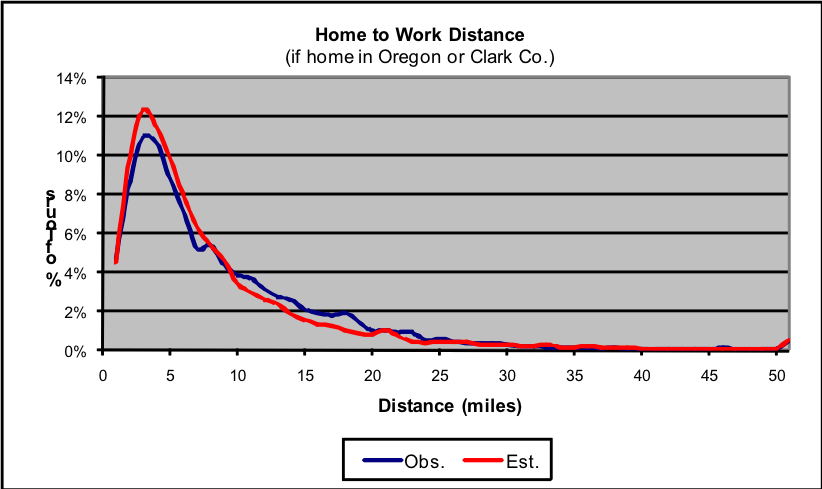
\includegraphics[width=4.5in]{pt/excel-figures/figure7-12.png}
\caption{Calibration results for home-to-work distance}
\label{fig:pt-home-work-distance-calibration}
\end{figure}

\subsubsection{Tour primary destination choice model}
This model has been calibrated to match average tour length by tour purpose, statewide and the percent of intrazonal tours, also statewide. The calibration consists of adjusting the coefficients for tour distance and for the intrazonal indicator variable. The comparison to the target data is shown in Table \ref{tab:average-tour-length-percent-intrazonal}.

% This table was marked as 7-68 in the text, but actually refers to Figure 7-12 (a table pasted in as a figure)
\begin{table}
\centering
\caption{Average tour length and percent intrazonal tours}\label{tab:average-tour-length-percent-intrazonal}
\begin{tabular}{lrrrrcrrr}
\hline
 & \multicolumn{4}{c}{Average tour length (miles)} &  & \multicolumn{3}{c}{Percent interzonal trips} \\
\cline{2-5}\cline{7-9}
Tour purpose & Target & Estimate & Error & \% error & & Target & Estimate & Error (\%) \\
\hline
School & 9.5 & 9.4 & -0.1 & -1.1 & & 16.3 & 15.2 & -1.0 \\
\gray College & 15.6 & 16.8 & 1.2 & 7.7 & & 6.1 & 5.5 & -0.6 \\
Shop & 14.4 & 14.6 & 0.2 & 1.4 & & 6.5 & 6.1 & -0.4 \\
\gray Recreation & 12.8 & 13.7 & 0.9 & 7.0 & & 11.4 & 10.9 & -0.5 \\
Other & 11.0 & 11.0 & 0.0 & 0.0 & & 9.1 & 8.3 & -0.8 \\
\gray Subtours & 8.1 & 8.3 & 0.2 & 2.5 & & 4.7 & 8.1 & 3.4 \\
\hline
\end{tabular}
\end{table}

\subsubsection{Tour schedule choice model}
This model has been calibrated to match the distribution of departure time and duration by tour purpose, statewide. The calibration consisted of adjusting the alternative-specific constants. The comparison to the target data is shown in Figures \ref{fig:pt-tour-departure-times-redux} (departure time) and \ref{fig:pt-tour-durations-redux} (duration). The model was also compared to several other targets:

\begin{sidewaysfigure}  % Figures 7.14 through 7.28
\centering
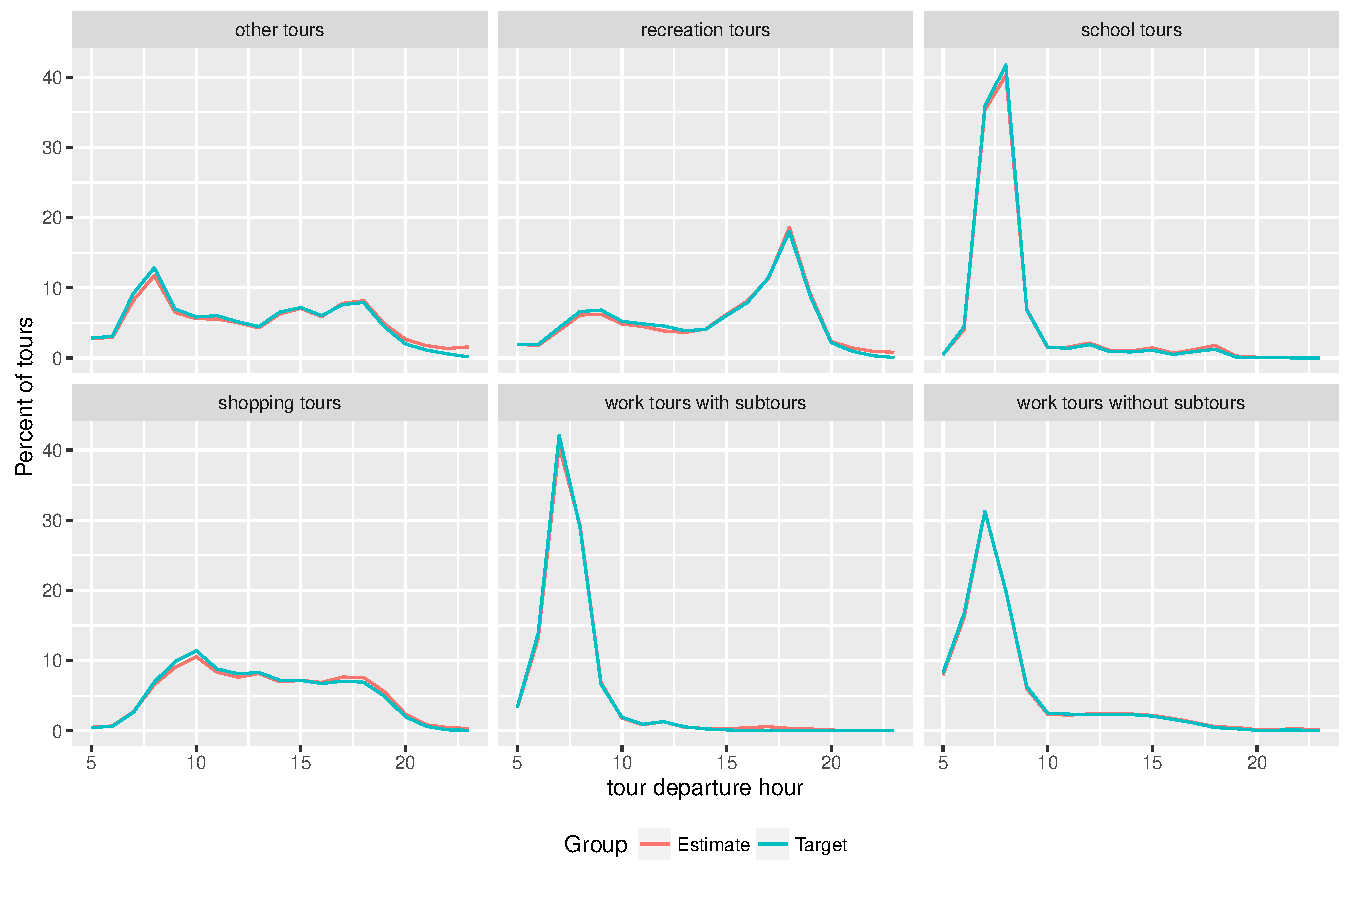
\includegraphics[scale=0.9]{pt/pt-tour-departure-hours-redux}
\caption{Observed versus estimated tour departure hours by tour type}
\label{fig:pt-tour-departure-times-redux}
\end{sidewaysfigure}

\begin{sidewaysfigure}  % Figures 7.19 through 7.23
\centering
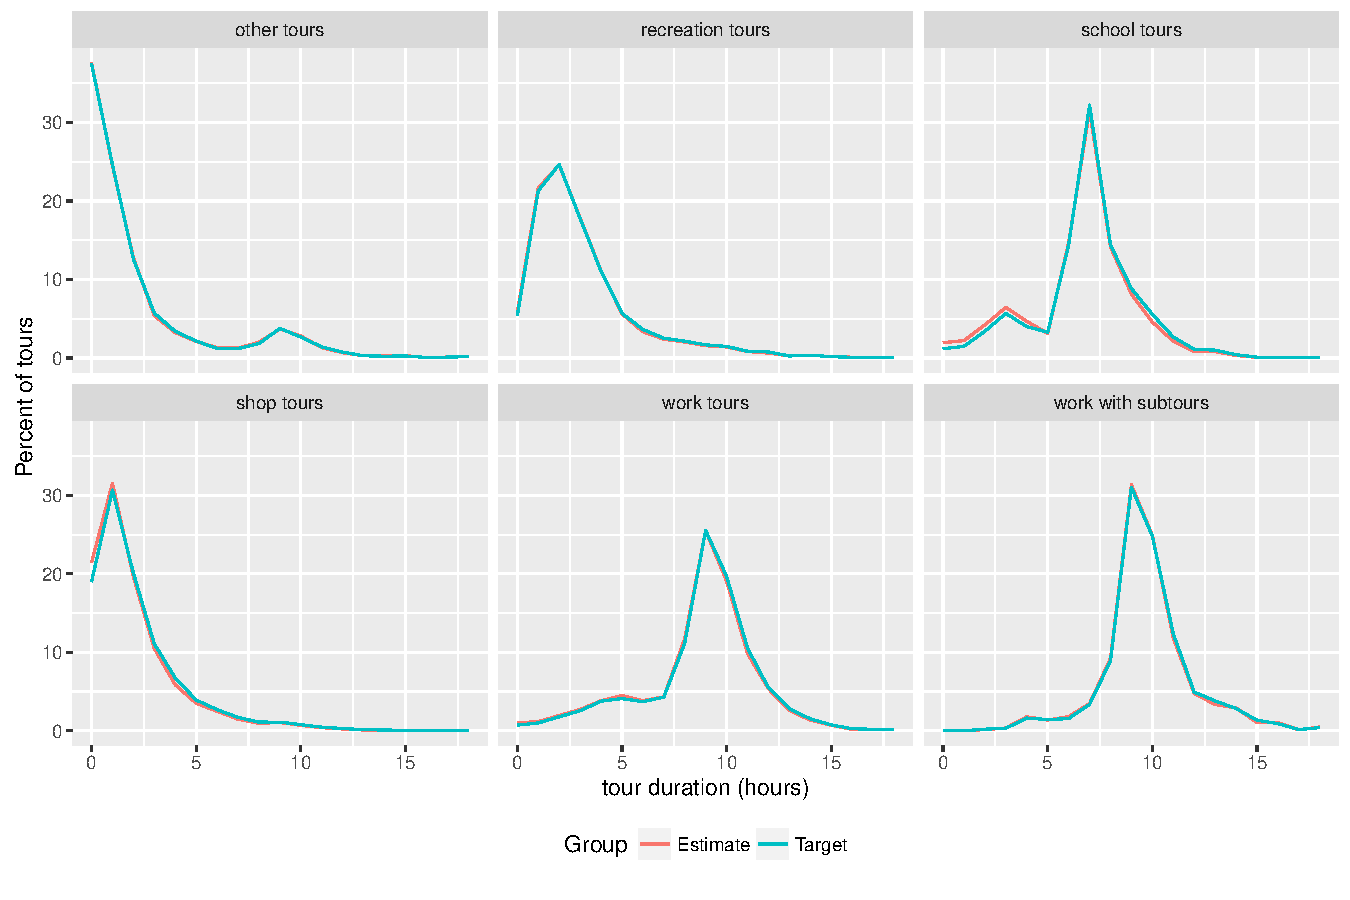
\includegraphics[scale=0.9]{pt/pt-tour-durations-redux}
\caption{Observed versus estimated tour durations by tour type}
\label{fig:pt-tour-durations-redux}
\end{sidewaysfigure}

\begin{itemize}
\item The auto ownership model was calibrated to match targets developed from the Oregon survey data. The number of households within the zero, one, two or three or more vehicles was matched within 2 percent of the target data statewide.
\item The PT SDT intermediate stop location model was calibrated to match average deviation distance by mode, percent of stops in the home alpha zone by mode and percent of stops in the primary destination alpha zone by mode. The calibration consists of adjusting the coefficients on out-of-direction time and intrazonal indicator variables. An initial calibration showed that the model was not able to reproduce observed differences in trip length by inbound/outbound stop. The model has been modified so that the time and intrazonal variables are now segmented by stop position; further calibration of these segmented parameters is underway.
\item The PT SDT intermediate stop duration model was calibrated to match the distribution of stop duration by tour purpose and stop position (outbound/inbound). The calibration consisted of adjusting the alternative-specific constants and the outbound stop indicator variable.
\item The PT SDT tour primary mode choice model was calibrated to the frequency of tours by market segment (car sufficiency). The calibration consists of adjusting the alternative-specific constants until each segment is within 10 percent of the target. 
\item The PT SDT trip mode choice model was calibrated to frequency of trips by primary mode. The calibration consists of adjusting the alternative-specific constants until each segment is within 10 percent of the target.
\end{itemize}

\subsection{LDT calibration}

\subsubsection{Binary choice of travel}
The results of the binary choice of travel model by purpose compared to the 1995 American Travel Survey calibration targets are shown in Table \ref{tab:ats-long-tours}. Overall, the highest rate of travel is for other tours, at 33 percent and the lowest is for work related tours, at four percent. According to the target data, the frequency of long distance travel is greater in Oregon than in Ohio, perhaps because of income and geographic differences.

\begin{table}
\centering
\caption{Percent of persons making long distance tour in a two-week period}\label{tab:ats-long-tours}
\begin{tabular}{lrrr}
\hline
Tour purpose & Observed & Modeled & Difference \\
\hline
Household & 16.8 & 17.9 & 1.1 \\
\gray Work-related & 3.8 & 4.1 & 0.3 \\
Other & 33 & 35.2 & 2.2 \\
\gray Total & 47.7 & 47.4 & -0.3 \\
\hline
\multicolumn{4}{l}{\footnotesize Note: All values shown are percentages.} \\
\end{tabular}
\end{table}

\subsubsection{Tour pattern}
While the LDT tour pattern model itself requires no calibration, when combined with the binary choice of travel model, it results in the total trips generated. The total number of long distance trips occurring on the travel day and the subset of those that are greater than 100 miles, summarized from the ATS, are shown in Table \ref{tab:ats-distances}.

\begin{table}
\centering
\caption{Total trips on model day}\label{tab:ats-distances}
\begin{tabular}{lrrrr}
\hline
Range & Observed & Modeled & Difference & \% difference \\
\hline
$>$50 miles &  & 257,152 &  &  \\
\gray $>$100 miles & 157,272 & 157,684 & 412 & 0.3 \\
\hline
\end{tabular}
\end{table}

\subsubsection{Scheduling}
The scheduling model draws from observed frequency distributions for beginning tours and ending tours, which is assumed to be the same in Oregon as in Ohio. No calibration was required for the departure time of beginning tours or the arrival time of ending tours. The modeled and observed departure times, as well as arrival times and durations for the complete tour scheduling model, are shown in Figures \ref{fig:pt-tour-departure-arrival-times} and \ref{fig:pt-complete-tours-duration}.

\begin{sidewaysfigure}  % Figures 7.24 and 7.25
\centering
\subfloat[Departure time for begin tours]{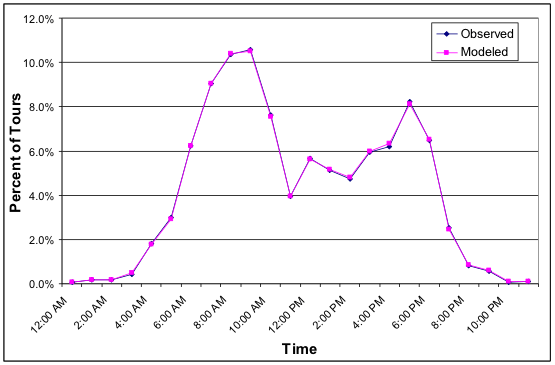
\includegraphics[width = 4in]{pt/excel-figures/figure7-24a.png}} 
\subfloat[Arrival time for end tours]{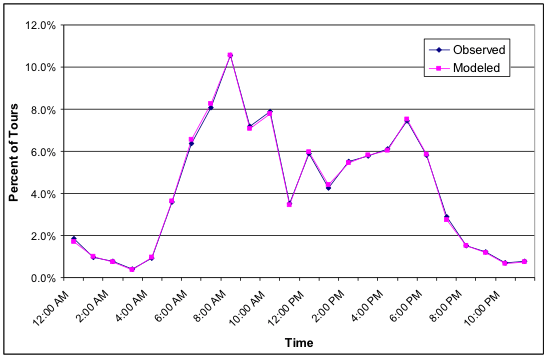
\includegraphics[width = 4in]{pt/excel-figures/figure7-24b.png}} \\
\subfloat[Departure time for complete tours]{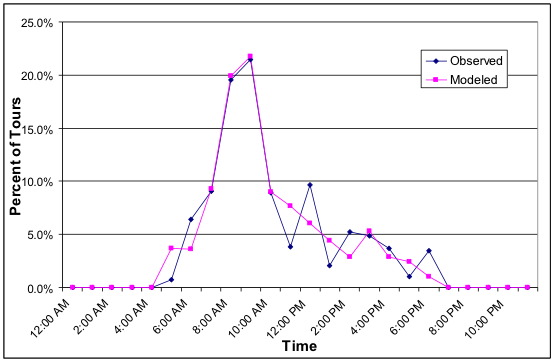
\includegraphics[width = 4in]{pt/excel-figures/figure7-25a.png}}
\subfloat[Arrival time for complete tours]{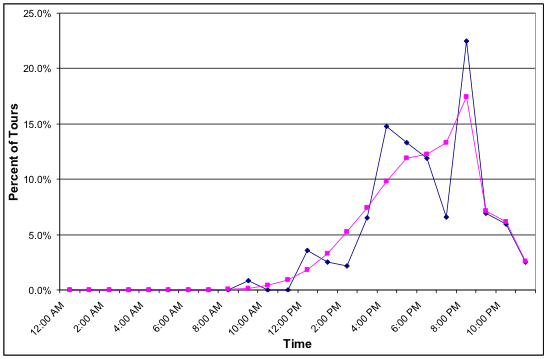
\includegraphics[width = 4in]{pt/excel-figures/figure7-25b.png}} 
\caption{Tour departure and arrival times}
\label{fig:pt-tour-departure-arrival-times}
\end{sidewaysfigure}

\begin{figure}   % Figure 7.26
\centering
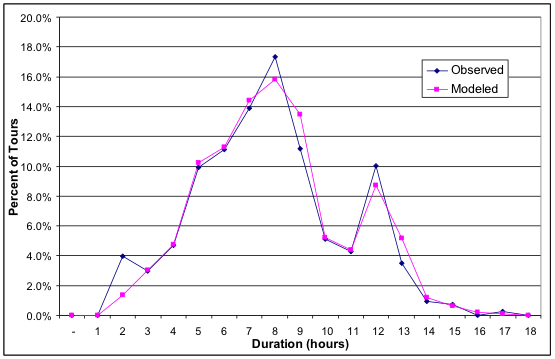
\includegraphics[width=4.25in]{pt/excel-figures/figure7-26.png}
\caption{Duration for complete tours}
\label{fig:pt-complete-tours-duration}
\end{figure}

\subsubsection{Internal-external choice}
The LDT internal-external choice models were calibrated to match the in-state versus out-of-state shares found in the ATS for trips longer than 100 miles. The model calibration results are shown in table \ref{tab:pt-internal-external-calibration}. Because the length of external trips is not known beyond the model area, all external trips are assumed to be longer than 100 miles for comparison to the ATS.

\begin{table}  % 7 68
\centering
\caption{Internal-external model calibration results}\label{tab:pt-internal-external-calibration}
\begin{tabular}{lrrrr}
\hline
 & \multicolumn{4}{c}{Trips $>$100 miles} \\
Trip type & Observed & Modeled & Difference & \% difference \\
\hline 
Internal & 64,836 & 67,282 & 2,446 & 3.8 \\
\gray External & 92,436 & 90,402 & -2,034 & -2.2 \\
Total & 157,272 & 157,684 & 412 & 0.3 \\
\hline
\end{tabular}
\end{table}

\subsubsection{Destination choice}
The LDT destination choice models are applied separately for internal versus external destinations. To calibrate the models, the distance flags were adjusted to properly match the number of trips in three distance bands: less than 60 miles, 60 to 70 miles and 70 to 150 miles. The inclusion of these distance band constants allows the model to match the observed trip length distributions without modifying the mode choice logsum coefficients. The observed trip lengths and trip length distributions are taken from the Ohio data, because no such information is available in the ATS. If data becomes available that is specific to Oregon, these models can be recalibrated. 

The modeled and observed average trip lengths are shown in Table \ref{tab:internal-destinations-average-distances}, while the modeled and observed trip length distributions by purpose are shown in Figure \ref{fig:pt-trip-length-distributions-destinations}. Due to relatively small sample sizes, the observed distributions are somewhat lumpy, but the models generally match those curves well.

\begin{table}   % 7 69
\centering
\caption{Average Trip lengths of tours with internal destinations}
\label{tab:internal-destinations-average-distances}
\begin{tabular}{llrrrr}
\hline
Tour type & Tour category & Observed & Modeled & Difference & \% difference \\
\hline
Household & Begin and end tours & 131.4 & 165 & 33.6 & 25.6 \\
\gray \cellcolor{white} & Complete tours & 89.4 & 97.4 & 8 & 8.9 \\
 & Total & 101.3 & 116.5 & 15.2 & 15 \\
\hline
\gray \cellcolor{white}Work-related & Begin and end tours & 130.6 & 155.5 & 24.9 & 19.1 \\
 & Complete tours & 90.8 & 98.9 & 8.1 & 8.9 \\
\gray \cellcolor{white} & Total & 97.5 & 108.4 & 10.9 & 11.2 \\
\hline
Other & Begin and end tours & 126.8 & 114 & -12.8 & -10.1 \\
\gray \cellcolor{white} & Complete tours & 92.1 & 92.7 & 0.6 & 0.7 \\
 & Total & 102.8 & 99.3 & -3.5 & -3.4 \\
\hline
\gray \cellcolor{white}All trips & Begin and end tours & 128.3 & 130.6 & 2.3 & 1.8 \\
 & Complete tours & 91.2 & 94.9 & 3.7 & 4.1 \\
\gray \cellcolor{white} & Total & 101.7 & 105 & 3.3 & 3.2 \\
\hline
\end{tabular}
\end{table}

\begin{sidewaysfigure}  % Figures 7.27 and 7.28
\centering
\subfloat[Household tours with internal destinations]{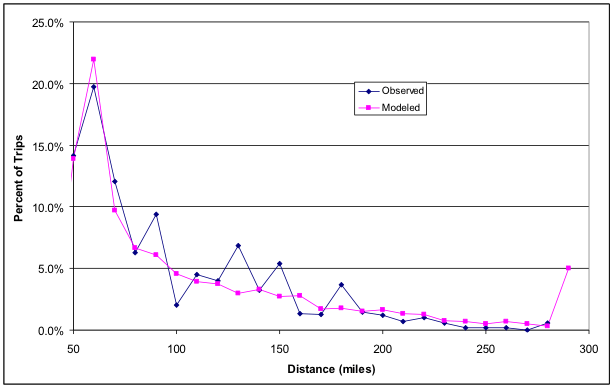
\includegraphics[width = 4in]{pt/excel-figures/figure7-27.png}} 
\subfloat[Work-related tours with internal destinations]{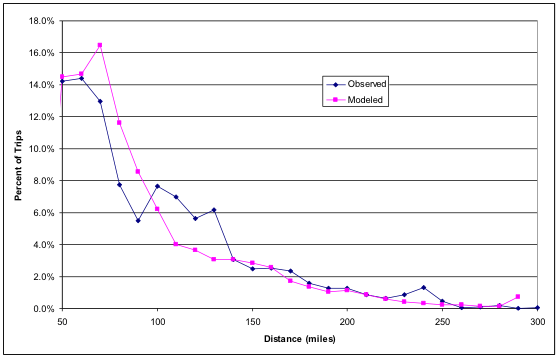
\includegraphics[width = 4in]{pt/excel-figures/figure7-28a.png}} \\
\subfloat[Work-related tours with external destinations]{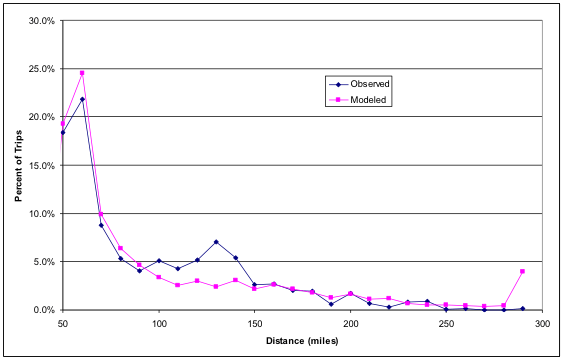
\includegraphics[width = 4in]{pt/excel-figures/figure7-28b.png}}
%\subfloat{
\includegraphics[width = 4in]{pt/excel-figures/empty-box.png}} 
\caption{Trip length distributions by destination type}
\label{fig:pt-trip-length-distributions-destinations}
\end{sidewaysfigure}

The modeled LDT external trips lengths do not compare well to the trip lengths observed in the Ohio survey, because they are truncated at the model boundary or external station. Therefore, the average modeled trip lengths are shown in Table \ref{tab:external-destination-modeled-distances} with no evaluation against observed data.

\begin{table}   % 7 70
\centering
\caption{Average modeled trip distances for tours with external destinations}
\label{tab:external-destination-modeled-distances}
\begin{tabular}{lrrr}
\hline
 & Begin and & Complete &  \\
Tour type & end tours & tours & ~~~~~~Total \\
\hline
Household & 172.0 & 165.2 & 170.2 \\
\gray Work-related & 167.7 & 167.2 & 167.6 \\
Other & 160.5 & 157.1 & 159.2 \\
\gray All trips & 166.0 & 160.9 & 164.4 \\
\hline
\end{tabular}
\end{table}
    
\subsubsection{Mode choice}
The mode choice models were calibrated to match the auto versus non-auto shares observed in the ATS for trips within Oregon. Unfortunately, inter-city transit and air skims are not available, so that calibration was not completed. For now, the air and transit alternatives are unavailable, such that all trips with internal destinations choose auto. This is a reasonable approximation because the observed data show 96 percent of long distance trips choosing auto. The current mode choice constants may change when the calibration is completed. Existing uncalibrated LDT mode choice outputs are shown in Table \ref{tab:results-100} by trip type.

\begin{table}
\centering
\caption{Mode choice calibration results for trips $>$100 miles}\label{tab:results-100}
\begin{tabular}{llrrr}
\hline
Category & Type & Internal & External & Total \\
\hline
Observed & Auto & 62,256 & 51,652 & 113,908 \\
\gray \cellcolor{white}& Non-Auto & 2,580 & 40,784 & 43,364 \\
& Total & 64,836 & 92,436 & 157,272 \\
\hline
\gray \cellcolor{white}Modeled & Auto & 67,282 & 50,458 & 117,740 \\
& Non-Auto & - & 39,944 & 39,944 \\
\gray \cellcolor{white}& Total & 67,282 & 90,402 & 157,684 \\
\hline
Difference & Auto & 5,026 & -1,194 & 3,832 \\
\gray \cellcolor{white}& Non-Auto & -2,580 & -840 & -3,420 \\
& Total & 2,446 & -2,034 & 412 \\
\hline
\gray \cellcolor{white}Percent difference & Auto & 8 & -2 & 3 \\
& Non-Auto & -100 & -2 & -8 \\
\gray \cellcolor{white}& Total & 4 & -2 & 0 \\
\hline
\end{tabular}
\end{table}
 
\subsubsection{Auto occupancy} 
During the calibration process, it was recognized as important to account for auto occupancy in order to get the number of auto vehicle trips correct. For work related and other tours, a simple model is applied to determine if an auto person trip becomes a vehicle trip by calculating the probability of being a vehicle trip as one divided by the average auto occupancy. For household tours, all household members travel together, so the auto occupancy is, by definition, the household size. The modeled and observed auto occupancies are shown in Table \ref{tab:average-occupancy}. The modeled household tour auto occupancy is somewhat lower than the observed value, indicating that the average size of households traveling is lower in the model than in the survey data. This is not considered a major issue because the number of vehicle trips is still correct. 

\begin{table}
\centering
\caption{Average auto occupancy}\label{tab:average-occupancy}
\begin{tabular}{lrrrr}
\hline
Tour type & Observed & Modeled & Difference & \% difference \\
\hline
Household internal & 2.79 & 2.24 & -0.55 & -19.7 \\
\gray Household external & 2.84 & 2.26 & -0.58 & -20.4 \\
Work-related internal & 1.21 & 1.22 & 0.01 & 0.8 \\
\gray Work-related external & 1.27 & 1.22 & -0.05 & -3.9 \\
Other internal & 1.86 & 1.91 & 0.05 & 2.7 \\
\gray Other external & 2.04 & 1.91 & -0.13 & -6.4 \\
\hline
\end{tabular}
\end{table}

\section{S3 Parameters}
PT is largely assumed to be fixed when the full SWIM2 system undergoes calibration. The one exception is the SDT workplace choice model $\lambda$ parameter, which can be adjusted to reflect the calibrated AA labor flow inputs. Other parameters may be revisited, if warranted.
